% (c)~2012 Dimitrios Vrettos - d.vrettos@gmail.com
% (c)~2014 Claudio.carboncinii - claudio.carboncini@gmail.com
\chapter{Equazioni di secondo grado}
\section{Le equazioni di secondo grado in una incognita}

Consideriamo il seguente problema: ``in un triangolo rettangolo l'ipotenusa è più lunga del cateto minore di $4\unit{cm}$, mentre l'altro cateto è più lungo del cateto minore di $2\unit{cm}$. Si vogliono determinare le misure dei tre lati''.

Si può formalizzare il problema indicando con $x$ la misura incognita del cateto minore. La lunghezza dell'ipotenusa sarà $x + 4$, mentre quella dell'altro cateto $x + 2$. Applicando il teorema di Pitagora si ha: $x ^{2 } + ( x + 2 ) ^{2 } = ( x + 4 ) ^{2 }$. Dopo aver effettuato i calcoli e aver portato tutti i termini a sinistra del predicato uguale abbiamo: $x ^{2}-4x-12=0$.
\begin{center}
% (c) 2013 Claudio Carboncini - claudio.carboncini@gmail.com
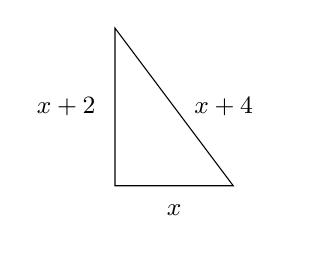
\begin{tikzpicture}[x=10mm,y=10mm,font=\small]
  \draw (1,1) -- (1,3) -- (2.5,1) -- cycle;
  \node [label={[name=label node]left:$x+2$}] at (1,2) {};
  \node [label={[name=label node]left:$x+4$}] at (3,2) {};
  \node [label={[name=label node]below:$x$}] at (1.75,1) {};
\end{tikzpicture}

\end{center}

Questa è una equazione di secondo grado in una incognita in quanto la variabile $x$ vi compare elevata al secondo grado.
\begin{definizione}
Si dice \emph{equazione di secondo grado}, un'equazione del tipo: $a x ^{2} + b x + c = 0$ con $a$, $b$, $c \in \insR$ e $a \neq 0$. I valori $a$, $b$, $c$ prendono il nome di \emph{coefficienti} e, in particolare, $c$ viene detto \emph{termine noto}.
\end{definizione}

Un'equazione di secondo grado si definisce:
\begin{description*}
 \item \emph{monomia} quando il secondo e il terzo coefficiente sono nulli: $\:a x ^{2}=0$;
 \item \emph{(incompleta) pura} quando il secondo coefficiente è nullo: $\:a x ^{2} + c = 0$;
 \item \emph{(incompleta) spuria} quando il terzo coefficiente è nullo: $\:a x ^{2} + b x = 0$;
 \item \emph{completa} quando i tre coefficienti sono tutti diversi da zero: $\:a x ^{2} + b x + c = 0$.
\end{description*}

\subsection{Risoluzione di un'equazione di secondo grado incompleta pura}

Il coefficiente della $x$ è nullo e l'equazione si presenta nella forma: $ax ^{2 } + c = 0$.
Si risolve portando al secondo membro il termine noto e dividendo per il coefficiente di $x^2$:
\[a x ^{2} + c = 0 \quad\Rightarrow\quad a x ^{2 } = - c \quad\Rightarrow\quad x
^{2} = - \frac{c }{a } \quad\Rightarrow\quad x _{1\text{,}2} = \pm \sqrt{- \frac{c}{a}}.\]
\pagebreak
\begin{exrig}
\begin{esempio}
 Risoluzione di equazioni pure.
\begin{itemize}
\item $4 x ^{2} - 9 =0$.

Risoluzione: $4 x ^{2 } = + 9 \:\Rightarrow\: x ^{2 } = \frac{9 }{4 }
\:\Rightarrow\: x _{1\text{,}2 } = \pm \sqrt{\frac{9 }{4 } } \:\Rightarrow\: x_{1} = - \frac{3 }{2 } \vee x _{2 } = + \frac{3 }{2 }$.
\item $4 x ^{2 } + 9 = 0$.

Risoluzione: $4 x ^{2 } = -9 \:\Rightarrow\: x ^{2 } = - \frac{9 }{4 }$. L'equazione non ammette soluzioni reali in quanto il quadrato di un numero reale non è mai negativo.
\end{itemize}
\end{esempio}
\end{exrig}

Le soluzioni dell'equazione incompleta pura $ax ^{2 } + c = 0$ dipendono dal segno di
$- \dfrac{c }{a }$:
\begin{itemize*}
\item se $-c/a>0$, ovvero se $a$ e $c$ sono discordi, l'equazione ammette \emph{due soluzioni reali distinte opposte}: $x _{1 } = - \sqrt{- \frac{c }{a}} \vee x_{2}= + \sqrt{-\frac{c}{a}}$;
\item se $-c/a<0$, ovvero se $a$ e $c$ sono concordi, l'equazione \emph{non ammette soluzioni reali};
\item se $-c/a=0$, allora $c =0$, l'equazione ha \emph{due soluzioni reali coincidenti nulle}: $x_{1}=x_{2} =0$.
\end{itemize*}

\vspazio\ovalbox{\risolvii \ref{ese:3.1}, \ref{ese:3.2}, \ref{ese:3.3}, \ref{ese:3.4}}

\subsection{Risoluzione di un'equazione incompleta spuria}

Un'equazione incompleta spuria si presenta nella forma: $a x ^{2} + b x = 0$.
Per risolverla, si raccoglie a fattore comune la
$x$; precisamente $x ( a x + b ) = 0$.
Applicando la legge di annullamento del prodotto si ottiene
$x_{1} = 0$ oppure $ax + b = 0$ da cui $x_{2} = - \dfrac{b}{a}$.
Pertanto un'equazione di questo tipo ha sempre due soluzioni reali distinte di cui una nulla.
\begin{exrig}
\begin{esempio}
Risoluzione di equazioni incomplete spurie.
\begin{itemize}
\item $2 x^{2} - 4 x = 0$.

Raccogliendo a fattor comune si ha: $2 x ( x - 2 ) = 0$ da cui, applicando la legge di annullamento del prodotto, segue $2x = 0 \vee x - 2 = 0$ da cui $x_{1} = 0 \vee x_{2} = 2$;
\item $x ^{2 } + x = 0$.

Raccogliendo $x$ a fattore comune, si ha $x ( x + 1 ) = 0$, da cui, applicando la legge di annullamento del prodotto, segue $x = 0 \vee x + 1 = 0$ da cui $x_{1} = 0 \vee x_{2} = - 1$.
\end{itemize}
\end{esempio}
\end{exrig}
\vspazio\ovalbox{\risolvii \ref{ese:3.5}, \ref{ese:3.6}, \ref{ese:3.7}, \ref{ese:3.8}}
\pagebreak
\section{Risoluzione di un'equazione completa}

L'equazione di secondo grado completa si presenta nella forma $a x ^{2} + b x = 0$ e per risolverla si applica una formula che si ottiene utilizzando il metodo del completamento del quadrato:

\begin{tabular}{ll}
equazione completa di secondo grado & $a x^{2} + b x + c=0$\\
si moltiplicano ambo i membri per $4a$ & $4 a^{2} x^{2} + 4 a b x + 4 a c=0$\\
si aggiunge $b^{2}$ ad ambo i membri & $4 a^{2} x^{2} + 4 a b x + 4 a c + b^{2}=b^{2}$\\
si porta $4ac$ al secondo membro & $4 a^{2} x^{2} + 4 a b x + b^{2}=b^{2} - 4 a c$\\
il primo membro risulta il quadrato di un binomio & $( 2 a x + b )^{2}=b^{2} - 4 a c$\\
si pone $k=2ax + b$ e l'equazione diventa pura in $k$ & $k^{2}=b^{2} - 4 a c$\\
si calcolano le soluzioni in $k$ & $k_{1\text{,}2}=\pm \sqrt{b^{2} - 4 a c}$\\
al posto di $k$ si sostituisce $2ax + b$ & $2 a x + b=\pm \sqrt{b^{2} - 4 a c}$\\
si separa il monomio con l'incognita & $2 a x=- b \pm \sqrt{b^{2} - 4 a c}$\\
si risolve rispetto all'incognita $x$ & $x_{1\text{,}2}=\dfrac{- b \pm \sqrt{b^{2} - 4 a c}}{2 a}$\\
\end{tabular}

%\begin{description*}
%\item $a x^{2} + b x + c=0$: equazione completa di secondo grado;
%\item $4 a^{2} x^{2} + 4 a b x + 4 a c=0$: si moltiplicano ambo i membri per $4a$;
%\item $4 a^{2} x^{2} + 4 a b x + 4 a c + b^{2}=b^{2}$: si aggiunge ad ambo i membri $b^{2}$;
%\item $4 a^{2} x^{2} + 4 a b x + b^{2}=b^{2} - 4 a c$: si porta $4ac$ a secondo membro;
%\item $( 2 a x + b )^{2}=b^{2} - 4 a c$: il primo membro risulta il quadrato di un binomio;
%\item $k=2 a x + b$: si sostituisce il binomio $2ax + b$ con la la variabile $k$;
%\item $k^{2}=b^{2} - 4 a c$: l'equazione diventa un'equazione di secondo grado pura in $k$;
%\item $k_{1,2}=\pm \sqrt{b^{2} - 4 a c}$: si calcolano le soluzioni in $k$;
%\item $2 a x + b=\pm \sqrt{b^{2} - 4 a c}$: al posto di $k$ si mette il binomio $2ax + b$;
%\item $2 a x=- b \pm \sqrt{b^{2} - 4 a c}$: si separa il monomio con l'incognita;
%\item $x_{1,2}=\frac{- b \pm \sqrt{b^{2} - 4 a c}}{2 a}$: si risolve l'equazione di primo grado rispetto alla $x$.
%\end{description*}

Da quanto ottenuto possiamo osservare che:
\begin{itemize}
\item la soluzione si ottiene esclusivamente operando sui coefficienti
dell'equazione;
\item il valore dell'incognita si ottiene con due calcoli:
\[x_{1} = \dfrac{- b - \sqrt{b^{2} - 4 ac}}{2 a}\quad\text{e}\quad x_{2} = \dfrac{- b + \sqrt{b^{2} - 4 ac}}{2 a}\;;\]
\item nel calcolo è coinvolta l'estrazione di radice quadrata: l'espressione $b^{2} - 4 ac$ prende il nome di \emph{discriminante} e si è soliti indicarla con il simbolo $\Delta$ (delta).
\end{itemize}

Questa formula può essere applicata anche ai tipi di equazioni incomplete che abbiamo già studiato. Il termine discriminante deriva dal sostantivo latino \emph{discrimen} (divisione, punto di separazione); in effetti, il valore assunto da $\Delta$ permette di effettuare una distinzione tra la tipologia delle soluzioni di un'equazione di secondo grado.
Si possono infatti presentare tre casi:
\begin{itemize}
\item Primo caso: $\Delta=b^{2} - 4 a c > 0$. Il radicale $\sqrt{\Delta}$ è un numero reale e l'equazione ammette \emph{due soluzioni reali e
distinte}: $x_{1}=\dfrac{- b - \sqrt{\Delta}}{2 a} \vee x_{2} = \dfrac{- b + \sqrt{\Delta}}{2 a}$;
\item Secondo caso: $\Delta=b^{2} - 4 a c=0$. Il radicale $\sqrt{\Delta} = 0$, quindi l'equazione ammette \emph{due radici reali e coincidenti}: $x_{1}=x_{2}=- \dfrac{b}{2 a}$;
\item Terzo caso: $\Delta=b^{2} - 4 a c < 0$. Il radicale $\sqrt{\Delta}$ non è un numero reale, quindi l'equazione \emph{non ammette soluzioni reali}.
\end{itemize}
\pagebreak
Riassumendo e schematizzando si ha:
\begin{center}
\begin{tabular}{ll}
\toprule
\multicolumn{2}{c} {$a x^{2} + b x + c=0$~~con~~$a \neq 0$}\vspace{1.05ex}\\
Discriminante & Soluzioni\\
\midrule
$\Delta > 0$ & Due soluzioni reali e distinte: $x_{1}=\frac{- b - \sqrt{\Delta}}{2 a} \vee x_{2} = \frac{- b + \sqrt{\Delta}}{2 a}$\\
$\Delta = 0$ & Due soluzioni reali e coincidenti: $x_{1}=x_{2}=- \frac{b}{2 a}$ \\
$\Delta < 0$ & Nessuna soluzione reale: $I.S.=\emptyset$ \\
\bottomrule
\end{tabular}
\end{center}
%\pagebreak
\begin{exrig}
\begin{esempio}
Risoluzione di equazioni complete.
\begin{itemize}
\item $3 x^{2} - 5 x + 2=0$.

 $a = + 3$, $b = - 5$, $c = + 2$. Calcolo del discriminante: 
\[\Delta = b^{2} - 4 ac = (-5)^{2}-4\cdot(+3)\cdot(+2) = 25 - 24 = 1.\]
 Poiché $\Delta > 0$ l'equazione ammette due soluzioni reali e distinte 
\[x_{1\text{,}2} = \frac{- b \pm \sqrt{\Delta}}{2 a} \:\Rightarrow\: x_{1\text{,}2} = \frac{- (- 5) \pm \sqrt{1}}{2\cdot(+3)} \:\Rightarrow\: x_{1\text{,}2} = \frac{5 \pm 1}{6} \:\Rightarrow\: x_{1} = 1 \vee x_{2} = \frac{2}{3};\]
\item $4 x^{2} - 12 x + 9=0$.

 $a = + 4$, $b = - 12$, $c = + 9$. Calcolo del discriminante: 
\[\Delta=(-12)^{2} -4\cdot(+4)\cdot(+9)=144 - 144 =0.\] 
Poiché $\Delta = 0$ l'equazione ammette due soluzioni reali coincidenti 
\[x_{1\text{,}2} = - \frac{b}{2 a} \:\Rightarrow\: x_{1\text{,}2} = \frac{-(-12)}{2\cdot(+4)} = \frac{12}{8} \:\Rightarrow\: x_{1} = x_{2} = \frac{3}{2};\]
\item $x^{2} - x + 3=0$.

 $a = + 1$, $b = - 1$, $c = + 3$. Calcolo del discriminante: 
\[\Delta = (-1)^{2} - 4\cdot(+1)\cdot(+3) = 1 - 12 = - 11.\]
Poiché $\Delta < 0$ l'equazione non ammette soluzioni reali.
\end{itemize}
\end{esempio}
\end{exrig}
\vspazio\ovalbox{\risolvii \ref{ese:3.9}, \ref{ese:3.10}, \ref{ese:3.11}\ref{ese:3.12}, \ref{ese:3.13}}

\subsection{Formula ridotta per equazioni di secondo grado}

Se nell'equazione
$a x^{2} + b x + c=0$ il coefficiente $b$ è un numero pari, conviene applicare una formula, detta \emph{formula ridotta}, che semplifica i calcoli.

Supponiamo $b=2 k$, l'equazione $a x^{2} + b x + c=0$ diventa $a x^{2} + 2 k x + c=0$ e nella formula risolutiva dell'equazione si ottiene:
\[x_{1\text{,}2}=\frac{- 2 k \pm \sqrt{( 2 k )^{2}-4 a c}}{2 a}=\frac{- 2 k \pm 2 \sqrt{k^{2} - a c}}{2 a}=\frac{- k \pm \sqrt{k^{2} - a c}}{a}.\]
Dato che $b=2 k$ si ha $k=\frac{b}{2}$ e quindi la formula che conviene utilizzare quando $b$ è pari è:
\[x_{1\text{,}2}=\frac{-\frac{b}{2} \pm \sqrt{\left(\frac{b}{2} \right)^{2} - a c}}{a}.\]

La quantità sotto radice, uguale a $\dfrac{\Delta}{4}$, è detta anche \emph{discriminante ridotto}.
%\pagebreak
\begin{exrig}
\begin{esempio}
 Applicazione della formula ridotta nella risoluzione di equazioni complete.
\begin{itemize}
\item $x^{2} - 4 x + 3=0$.

 Il coefficiente di primo grado è pari, per cui conviene utilizzare la formula ridotta: 
\[x_{1\text{,}2}=\frac{-(-2 ) \pm \sqrt{(-2)^{2}-1\cdot(+3)}}{1}=2 \pm \sqrt{1}\:\Rightarrow\:  x_{1} = 1 \vee x_{2} = 3;\]
\item $- x^{2} - 2 x + 24=0$.

 Applichiamo la formula ridotta: 
\[x_{1\text{,}2}=\frac{- ( - 1 ) \pm \sqrt{( -1 )^{2} - (-1)\cdot(+24)}}{-1}=- 1 \pm \sqrt{25}\:\Rightarrow\: x_{1} = - 6 \vee x_{2} = 4;\]
\item $- 3 x^{2} - 6 x + 12=0$.

 Per prima cosa dividiamo l'equazione per $- 3$. Per il secondo principio di equivalenza, si ha l'equazione equivalente~$x^{2} + 2 x - 4=0$. Poiché il coefficiente della~$x$ è pari si può applicare la formula ridotta: 
\[x_{1\text{,}2}=- 1 \pm \sqrt{1 + 4} = - 1\pm \sqrt{5}\:\Rightarrow\: x_{1} = - 1 + \sqrt{5} \vee x_{2} = - 1 - \sqrt{5}.\]
\end{itemize}
\end{esempio}
\end{exrig}

Quando $b$ è pari e $a = 1$, la formula si dice \emph{ridottissima}: $x_{1\text{,}2}=-\frac{b}{2} \pm \sqrt{\left( \frac{b}{2} \right)^{2} - c}$.
%\newpage
\begin{exrig}
\begin{esempio}
 Applicazione della formula ridottissima nella risoluzione di equazioni complete.
\begin{itemize}
\item $x^{2} - 6 x + 8 = 0$.

Il coefficiente $b$ è pari e il coefficiente $a=1$, quindi possiamo applicare la formula ridottissima $x_{1\text{,}2} = 3 \pm \sqrt{9 - 8}$, quindi $x_{1}=2 \vee x_{2} = 4$.
\end{itemize}
\end{esempio}
\end{exrig}
\vspazio\ovalbox{\risolvii  \ref{ese:3.14}, \ref{ese:3.15}} %\vspazio

\pagebreak
Riassumiamo e schematizziamo la risoluzione di un'equazione di secondo grado:
\begin{center}
\begin{tabular}{llll}
\toprule
\multicolumn{4}{c} {Equazioni incomplete}\vspace{1.05ex}\\
Coefficienti & Tipo & Equazione & Soluzioni\\
\midrule
$b = 0$, $c = 0$ & Monomia & $a x^{2}=0$ & $x_{1}=x_{2}=0$\\
$b = 0$, $c \neq 0$ & Pura & $a x^{2} + c=0$ & $\begin{cases} \IS=\emptyset & \text{ se~~}ac>0 \\ x_{1\text{,}2} = \pm \sqrt{- \frac{c}{a}} & \text{ se~~}ac<0\\ \end{cases}$ \\
% $b = 0$, $c \neq 0$ & Pura & $a x^{2} + c=0$ & \IS=\emptyset $ se $ac>0$\\
% & & & $x_{1\text{,}2} = \pm \sqrt{- \frac{c}{a}}$~~se~$a \cdot c<0$\\
$b \neq 0$, $c = 0$ & Spuria & $a x^{2} + b x=0$ & $x_{1} = 0 \vee x_{2} = - \frac{b}{a}$ \vspace{1.1ex}\\
\toprule
\multicolumn{4}{c} {Equazione completa \, $ax^2+bx+c=0$}\vspace{1.05ex}\\
Discriminante & \multicolumn{2}{l} {Numero soluzioni} & Soluzioni\\
\midrule
$\Delta > 0$ & \multicolumn{2}{l} {Due soluzioni reali e distinte}& $x_{1\text{,}2}=\frac{-b\pm{\sqrt {b^{2}-4ac}}}{2a}$\\
$\Delta = 0$ & \multicolumn{2}{l} {Due soluzioni reali e coincidenti} & $x_{1}=x_{2}=-\frac{b}{2a}$\\
$\Delta < 0$ & \multicolumn{2}{l} {Nessuna soluzione reale}& $\IS=\emptyset$\\
\bottomrule
\end{tabular}
\end{center}

\vspazio\ovalbox{\risolvii \ref{ese:3.16}, \ref{ese:3.17}, \ref{ese:3.18}, \ref{ese:3.19}, \ref{ese:3.20}, \ref{ese:3.21}, \ref{ese:3.22}, \ref{ese:3.23}, \ref{ese:3.24}, \ref{ese:3.25}, \ref{ese:3.26}, \ref{ese:3.27}, \ref{ese:3.28}, }

\vspazio\ovalbox{\ref{ese:3.29}, \ref{ese:3.30}, \ref{ese:3.31}, \ref{ese:3.32}}

\subsection{Equazioni che si possono risolvere con opportune sostituzioni}

\begin{exrig}
\begin{esempio}
Risoluzione di equazioni con sostituzioni.
\begin{itemize}
\item $( x - 1 )^{2} = 16$.

Sostituendo $x - 1 = t$ l'equazione diventa $t^{2} = 16$, le cui soluzioni sono $t_{1} = - 4 \vee t_{2} = + 4$. Per determinare la $x$ sostituiamo i valori di $t$ trovati nella relazione~$x - 1 = t$. Si ha $x - 1 = - 4 \vee x - 1 = + 4$ quindi l'equazione assegnata ammette le due soluzioni
$x_{1} = - 3 \vee x_{2} = 5$;
\item $( x - 1 )^{2} + 2 ( x - 1 ) = 0$.

Sostituendo $x - 1 = t$ l'equazione diventa $t^{2} + 2t = 0$ le cui soluzioni sono $t ( t + 2 ) = 0 \Rightarrow t_{1} = 0 \vee t + 2 = 0 \Rightarrow t_{2} = - 2$. Sostituendo $x - 1 = t$ si ha $x - 1 = 0 \vee x - 1 = - 2$ quindi l'equazione assegnata ammette le due soluzioni~$x_{1} = - 1 \vee x_{2} = 1$.
\end{itemize}
\end{esempio}
\end{exrig}
\vspazio\ovalbox{\risolvii \ref{ese:3.33}, \ref{ese:3.34}, \ref{ese:3.35}}
\pagebreak
\section{Discussione e risoluzione di equazioni numeriche frazionarie}

Un'equazione in cui compare l'incognita al denominatore si chiama \emph{frazionaria o fratta.}

\begin{exrig}
\begin{esempio}
Risolvere la seguente equazione:~~$\dfrac{3 x + 2}{1 + x}=\dfrac{2 x + 3}{x - 2}$.
 \paragraph{Passo I} Determiniamo il $\mcm$ dei denominatori: $\mcm = ( 1 + x ) \cdot ( x - 2 )$.
 \paragraph{Passo II} Imponiamo le \emph{condizioni di esistenza} ($\CE$): $\CE\: x \neq - 1 \wedge x \neq 2$. La ricerca dei valori che risolvono l'equazione si restringe ai numeri reali appartenenti all'insieme, $\Dom = \insR - \{-1$, $2\}$ detto \emph{dominio} dell'equazione o \emph{insieme di definizione} (abbreviato $\ID$).
 \paragraph{Passo III} Applichiamo il primo principio d'equivalenza trasportando al primo membro la frazione del secondo membro $\frac{3 x + 2}{1 + x} - \frac{2 x + 3}{x - 2} = 0$. Riduciamo allo stesso denominatore ($\mcm$): 
\[\frac{( 3 x + 2 ) \cdot ( x - 2 ) - ( 2 x + 3 ) \cdot ( 1 + x )}{( 1 +x ) \cdot ( x - 2 )}=0.\]
 \paragraph{Passo IV} Moltiplichiamo ambo i membri per il $\mcm$, certamente diverso da zero per le condizioni poste; l'equazione diventa: $( 3 x + 2 ) \cdot ( x - 2 ) - ( 2 x + 3 ) \cdot ( 1 + x )=0$.
 \paragraph{Passo V} L'equazione che si ottiene è di secondo grado; portiamo l'equazione alla forma canonica: $3 x^{2} - 6 x + 2 x - 4 - 2 x - 3 - 2 x^{2} - 3 x=0 \:\Rightarrow\: x^{2} - 9 x - 7=0$.
 \paragraph{Passo VI} Calcoliamo il discriminante: $\Delta=b^{2} - 4 a c=81 + 28 = 109$. Il discriminante è positivo quindi l'equazione è determinata e ammette due soluzioni reali distinte: 
\[x_{1\text{,}2}=\frac{9 \pm \sqrt{109}}{2} \quad\Rightarrow\quad x_{1}=\frac{9 - \sqrt{109}}{2} \:\vee\: x_{2}=\frac{9 + \sqrt{109}}{2}.\]
 \paragraph{Passo VII} Confrontiamo le soluzioni con le $\CE$; in questo caso le radici appartengono all'insieme $\Dom$; diciamo che sono accettabili e l'insieme soluzione è: $\IS=\left\{\frac{9 - \sqrt{109}}{2}\text{, }\frac{9 +\sqrt{109}}{2} \right\}$.
 \end{esempio}

 \begin{esempio}
Risolvere la seguente equazione:~~$\dfrac{x^{2}}{x^{2} - 3 x + 2}=\dfrac{x - 2}{x - 1} +\dfrac{1}{x + 2}$.
 \paragraph{Passo I} Determiniamo il $\mcm$ dei denominatori. Scomponiamo in fattori i denominatori. Riscriviamo: $\frac{x^{2}}{( x - 2 ) ( x - 1 )}=\frac{x - 2}{x - 1} +\frac{1}{x + 2}$ il $\mcm$ è $( x - 2 ) ( x - 1 ) ( x + 2 )$.
 \paragraph{Passo II} Imponiamo le Condizioni di Esistenza: $\CE\: x \neq 1 \wedge x \neq 2 \wedge x \neq - 2$ quindi $\Dom = \ID =\insR - \{-2$, $1$, $2\}$
 \paragraph{Passo III} Trasportiamo al primo membro ed uguagliamo a zero; riduciamo allo stesso denominatore ($\mcm$) i membri dell'equazione: 
\[\frac{x^{3} + 2 x^{2} - x^{2} + 3 x - 2 - x^{3} - 2 x^{2} + 4x^{2} + 8 x - 4 x - 8}{( x - 2 ) ( x - 1 ) ( x + 2 )} = 0.\]
 \paragraph{Passo IV} Applichiamo il secondo principio di equivalenza moltiplicando ambo i membri per il $\mcm$, certamente diverso da zero per le condizioni poste in precedenza; l'equazione diventa: $3 x^{2} + 7 x - 10 = 0$.
 \paragraph{Passo V} Calcoliamo il discriminante: $\Delta=b^{2} - 4 a c=49 + 120=169$. Il discriminante è positivo, l'equazione determinata e ammette due soluzioni reali distinte: $x_{1\text{,}2}=\frac{- 7 \pm 13}{6}$ cioè~$x_{1}=-\frac{10}{3} \vee x_{2}=1$.
 \paragraph{Passo VI} Confrontiamo con le $\CE$; in questo caso solo $x_{1}$ appartiene all'insieme $\Dom$; diciamo che l'insieme soluzione è: $\IS=\left\{-\frac{10}{3}\right\}$ mentre $x_{2} = 1$ non è accettabile.
\end{esempio}
\end{exrig}
\vspazio\ovalbox{\risolvii \ref{ese:3.36}, \ref{ese:3.37}, \ref{ese:3.38}, \ref{ese:3.39}, \ref{ese:3.40}, \ref{ese:3.41}, \ref{ese:3.42}, \ref{ese:3.43}, \ref{ese:3.44}, \ref{ese:3.45}, \ref{ese:3.46}, \ref{ese:3.47},}

\vspazio\ovalbox{\ref{ese:3.48}, \ref{ese:3.49}, \ref{ese:3.50}, \ref{ese:3.51},\ref{ese:3.52}, \ref{ese:3.53}, \ref{ese:3.54},\ref{ese:3.55}, \ref{ese:3.56}, \ref{ese:3.57}}

\section{Discussione e risoluzione di equazioni letterali}
Ricordiamo la seguente definizione:
\begin{definizione}
Una equazione è \emph{letterale} se i coefficienti dell'incognita sono espressioni letterali, cioè se oltre all'incognita (in genere indicata con
la lettera $x$) compare un'altra lettera (in genere $a$, $b$, $k$, \ldots) detta \emph{parametro}.
\end{definizione}

\begin{exrig}
\begin{esempio}
Data l'equazione $k x^{2} - ( 2 k - 1 ) x + ( k - 3 ) = 0$, discutere, al variare di $k$, la realtà delle sue soluzioni.

L'equazione è letterale di secondo grado nell'incognita $x$, i cui coefficienti dipendono dal parametro $k$. Il parametro $k$ può assumere qualunque valore numerico e l'equazione rappresenta una famiglia di equazioni le cui caratteristiche variano a seconda dei valori attribuiti al parametro. Notiamo subito che se
$k$ assume il valore zero, l'equazione non è più di secondo grado. Se $k$ assume il valore $3$, l'equazione è ancora di secondo grado ma è incompleta (spuria) perché priva del termine noto.

\emph{Discutere} un'equazione letterale significa analizzare come varia il suo insieme delle soluzioni al variare del parametro.

Ricordando la formula $x_{1\text{,}2}=\frac{- b \pm \sqrt{b^{2} - 4 a c}}{2 a}$ in cui compaiono i tre coefficienti $a$, $b$, $c$ possiamo dire che, nel caso considerato:
 \begin{itemize*}
 \item il primo coefficiente è $k$, se $k = 0$ l'equazione diventa $x - 3 = 0$ di primo grado con $\IS = \{3\}$;
 \item il secondo coefficiente è $-2k+1$, se questo è nullo, ossia se $k = \frac{1}{2}$ l'equazione diventa $\frac{1}{2} x^{2} - \frac{5}{2}=0$, equazione pura con due soluzioni reali opposte $x_{1} = - \sqrt{5} \vee x_{2} = \sqrt{5}$;
 \item il terzo coefficiente è $k-3$, se è nullo, cioè se $k = 3$ l'equazione diventa $3 x^{2} - 5 x = 0$, equazione spuria con due soluzioni reali $x_{1} = 0 \vee x_{2} = \frac{5}{3}$.
 \end{itemize*}
\pagebreak
Per tutti i valori di $k \in \insR - \left\{ 0\text{, }\frac{1}{2}\text{, }3 \right\}$ l'equazione è completa, pertanto l'esistenza di soluzioni reali dipende dal discriminante $\Delta = \left( - 2 k + 1 \right)^{2} - 4 k \left( k - 3 \right) = 8 k + 1$, quindi
\begin{itemize*}
 \item se $8 k + 1 < 0 \:\Rightarrow\: k < - \frac{1}{8}$ l'equazione non ammette soluzioni reali: $\IS = \emptyset$;
 \item se $8 k + 1 > 0 \:\Rightarrow\: k > - \frac{1}{8}$ l'equazione ammette due soluzioni reali distinte $ x_{1\text{,}2} = \frac{\left(2 k - 1 \right) \pm \sqrt{8 k + 1}}{2 k}$
 \item se $k=- \frac{1}{8}$ l'equazione ammette due soluzioni reali coincidenti $ x_{1} = x_{2}=5$.
\end{itemize*}
Riassumendo e schematizzando si ha:
\begin{center}
\begin{tabular}{lll}
\toprule
\multicolumn{3}{c} {$k x^{2} - ( 2 k - 1 ) x + ( k - 3 ) = 0$~~con~~$k \in \insR$}\vspace{1.05ex}\\
Parametro & Insieme Soluzione & Equazione\\
\midrule
$k = 0$ & $x = 3$ & di primo grado\\
$k = \frac{1}{2}$ & $x_{1} = - \sqrt{5} \vee x_{2} = + \sqrt{5}$ & pura\\
$k = 3$ & $x_{1} = 0 \vee x_{2} = \frac{5}{3}$ & spuria\\
$k \in \insR - \left\{ 0\text{, }\frac{1}{2}\text{, }3 \right\}$ & & completa, $\Delta = 8 k + 1$\\
$k < - \frac{1}{8}$ & $\Delta < 0$ non esistono soluzioni reali, $I.S. = \emptyset$& \\
$k \geq - \frac{1}{8}$ & $\Delta \geq 0$ esistono soluzioni reali & \\
$k > - \frac{1}{8}$ & $x_{1}=\frac{\left( 2 k - 1 \right) - \sqrt{8 k + 1}}{2k}\vee x_{2}=\frac{\left( 2 k - 1 \right) + \sqrt{8 k + 1}}{2 k}$ & \\
$k = - \frac{1}{8}$ & $x_{1} = x_{2}=5$ &\\
\bottomrule
\end{tabular}
\end{center}
\end{esempio}

\begin{esempio}
Data l'equazione $x^2 - 3 x + 1 - k = 0$, discutere, al variare di $k \in \insR$, la realtà delle radici.

Il primo e il secondo coefficiente non dipendono dal parametro $k$, quindi analizziamo il terzo coefficiente. Se $k = 1$ l'equazione diventa un'equazione spuria con due radici reali $x_{1} = 0 \vee x_{2} = 3$. Per tutti i valori di $k$ dell'insieme $\insR - \{1\}$ l'equazione è completa e l'esistenza di soluzioni reali dipende dal discriminante $\Delta = 9 - 4 ( 1 - k ) = 4 k + 5$, quindi:
\begin{itemize*}
 \item se $k < - \frac{5}{4}$ l'equazione non ammette soluzioni reali: $\IS = \emptyset$;
 \item se $k \geq - \frac{5}{4}$ l'equazione ammette due radici reali. Esse sono distinte se $k >-\frac{5}{4}\:\Rightarrow\: x_{1\text{,}2} =\frac{3 \pm\sqrt{4 k +5}}{2}$ e coincidenti se $k=- \frac{5}{4} \:\Rightarrow\: x_{1} = x_{2} = \frac{3}{2}$.
\end{itemize*}
Riassumendo e schematizzando si ha:
\begin{center}
\begin{tabular}{lll}
\toprule
\multicolumn{3}{c} {$x^{2} - 3 x + 1 - k = 0$~~con~~$k \in \insR$}\vspace{1.05ex}\\
Parametro & Insieme Soluzione & Equazione\\
\midrule
$k = 1$ & $x_{1} = 0 \vee x_{2} = 3$ & spuria\\
$k \in \insR - \{1\}$ & & completa, $\Delta = 4 k + 5$\\
$k < - \frac{5}{4}$ & $\Delta < 0$ non esistono soluzioni reali, $I.S. = \emptyset$& \\
$k \geq - \frac{5}{4}$ & $\Delta \geq 0$ esistono soluzioni reali & \\
$k > - \frac{5}{4}$ & $x_{1}=\frac{3 - \sqrt{4 k + 5}}{2} \vee x_{2}=\frac{3 + \sqrt{4 k + 5}}{2}$ & \\
$k = - \frac{5}{4}$ & $x_{1} = x_{2}=\frac{3}{2}$ &\\
\bottomrule
\end{tabular}
\end{center}
\end{esempio}
\pagebreak
\begin{esempio}
Discutere l'equazione letterale:~~$\dfrac{x^{2}}{m - 1} + 3 + m=\dfrac{2 m x}{m - 1} \left( 1 +\dfrac{1}{m} \right)$.

L'equazione, pur presentando delle frazioni, è intera in quanto l'incognita $x$ non compare al denominatore. Se~$m = 0$ oppure~$m = 1$ l'equazione è priva di significato, quindi poniamo $\CE\: m \neq 0 \wedge m \neq 1$.

Trasportiamo a sinistra del segno di uguaglianza i termini di destra ed eseguiamo il calcolo nella parentesi: 
\[\frac{x^{2}}{m - 1} + 3 + m - \frac{2 m x}{m - 1} \left( 1 +\frac{1}{m} \right) = 0 \:\Rightarrow\: \frac{x^{2}}{m - 1} + 3 + m - \frac{2 m x}{m - 1} - \frac{2 \cancel{m} x}{m - 1} \cdot \frac{1}{\cancel{m}} = 0.\]
Semplifichiamo $m$ nell'ultimo termine, poiché nelle $\CE m \neq 0$, si ottiene
\[\frac{x^{2}}{m - 1} + 3 + m - \frac{2 mx}{m - 1} - \frac{2 x}{m - 1}=0.\]
Riduciamo allo stesso denominatore $m - 1$ ed eliminiamo il denominatore, essendo $m \neq 1$ per le $\CE$; si ha: $x^{2} + 3 m - 3 + m^{2} - m - 2 m x - 2 x = 0$, che scritta in forma canonica diventa $x^{2} - 2 x ( m + 1 ) + m^{2} + 2 m - 3 = 0$.

\emph{Discussione}
\begin{itemize*}
\item il primo coefficiente, essendo uguale a $1$, non dipende dal valore del parametro~$m$, quindi l'equazione è di secondo grado per qualunque valore di $m \in \insR - \{0$, $1\}$;
\item il secondo coefficiente è $- 2 (m + 1)$: se $m = - 1$ l'equazione diventa $x^{2} - 4 = 0$, equazione pura con due soluzioni reali opposte $x_{1} = - 2 \vee x_{2} = 2$;
\item il terzo coefficiente è $m^{2} + 2 m - 3$: se $m^{2} + 2 m - 3 = 0 \:\Rightarrow\: m = 1 \vee m = - 3$ (non consideriamo il caso $m = 1$ per le $\CE$) l'equazione diventa $x^{2} + 4 x = 0$, equazione spuria con due soluzioni reali $x_{1} = 0 \vee x_{2} = - 4$.
\end{itemize*}
Prima conclusione: per tutti i valori di $m \in \insR -\{0$, $1$, $-1$, $-3\}$ l'equazione è completa e l'esistenza di soluzioni reali dipende dal discriminante. Calcoliamo il discriminante: $\frac{\Delta}{4} = ( m + 1 )^{2} - ( m^{2} + 2 m - 3 ) = 4$; esso risulta indipendente dal valore del parametro~$m$ e sempre positivo, quindi l'equazione ammette sempre due soluzioni reali distinte $x_{1} = m - 1 \vee x_{2} = m + 3$.

Riassumendo in una tabella tutti i risultati ottenuti:
\begin{center}
\begin{tabular}{lll}
\toprule
\multicolumn{3}{c} {$\frac{x^{2}}{m - 1} + 3 + m=\frac{2 m x}{m - 1} \left( 1 + \frac{1}{m} \right)$~~con~~$m \in \insR$}\vspace{1.05ex}\\
Parametro & Insieme Soluzione & Equazione\\
\midrule
$m = 0 \vee m=1$ & & priva di significato\\
$m =-1$ & $x_{1}=- 2 \vee x_{2}=2$ & pura\\
$m = -3$ & $x_{1}=0 \vee x_{2}=- 4$ & spuria\\
$m \in \insR - \{0$, $1$, $-1$, $-3\}$ & $x_{1} = m - 1 \vee x_{2} = m + 3$ & completa: $\Delta = 16$\\
\bottomrule
\end{tabular}
\end{center}
\end{esempio}
\pagebreak
\begin{esempio}
Discutere l'equazione parametrica~$\dfrac{k + x}{2 x} \left( \dfrac{k + x}{k - x} + \dfrac{k - x}{k + x} \right)=k + \dfrac{2 k}{k x - x^{2}} - 1$.

L'equazione è fratta, poiché l'incognita $x$ compare nel denominatore. Trasportiamo i termini del secondo membro a sinistra del segno di uguaglianza e scomponiamo in fattori i denominatori: 
\[\frac{k + x}{2 x} \left( \frac{k + x}{k - x} + \frac{k - x}{k +x} \right) - k - \frac{2 k}{x ( k - x )} + 1=0\qquad \CE\: x \neq 0 \wedge x \neq k \wedge x \neq - k.\]
Svolgiamo i calcoli nella parentesi e moltiplichiamo: $\frac{k^{2} + x^{2}}{x ( k - x )} - k - \frac{2 k}{x ( k - x )} + 1=0$;
Riduciamo allo stesso denominatore ed eliminiamo il denominatore: $k x^{2} + k x \cdot ( 1 - k ) + k \cdot ( k - 2 )=0$;

\emph{Discussione}
\begin{itemize}
 \item Il primo coefficiente è $k$, se $k = 0$ le $\CE$ si riducono a $x \neq 0$ e l'equazione diventa $0x = 0$ indeterminata, quindi $I.S. = \insR - \{ 0\}$ per le condizioni poste sull'incognita. Avendo studiato il caso $k=0$, possiamo ora supporre $k \neq 0$. Dividiamo tutti i coefficienti per $k$, l'equazione diventa $x^{2} + x \cdot ( 1 - k ) + ( k - 2 )=0$;
 \item il secondo coefficiente è $1-k$, se $k = 1$ le $\CE$ sono $x \neq 0 \wedge x \neq 1 \wedge x \neq - 1$ e l'equazione diventa $x^{2} - 1 = 0$, le soluzioni sono $x_{1} = -1 \vee x_{2} = 1$ che non sono accettabili per le $\CE$;
 \item il terzo coefficiente è $k-2$, se $k = 2$ le $\CE$ sono $x \neq 0 \wedge x \neq 2 \wedge x \neq - 2$ e l'equazione diventa $x^{2} - x = 0$ le cui soluzioni sono $x_{1} = 0 \vee x_{2} = 1$ di cui $x_{1} = 0$ non è accettabile per le $\CE$
\end{itemize}
Per $k \in \insR - \{0$, $1$, $2\}$ l'equazione è completa, l'esistenza di soluzioni reali dipende dal discriminante $\Delta = (1 - k)^{2}-4(k-2)=(k-3)^{2}$, essendo
$\Delta \geq 0\; \forall k$, si avranno sempre due soluzioni reali: coincidenti se $k = 3 \:\Rightarrow\: x_{1} = x_{2} = 1$ accettabili essendo le
$\CE\: x \neq - 3 \wedge x \neq 0 \wedge x \neq 3$; distinte se $k \neq 3 \:\Rightarrow\: x_{1} = 1 \vee x_{2} = k - 2$ e, confrontando con le $\CE$, si $x_{1} = 1$
non è accettabile se $k = - 1$, mentre $x_{2}$ è sempre accettabile per $\forall k \in \insR - \{0$, $1$, $2$, $3$, $-1\}$.

Riassumendo in una tabella tutti i risultati ottenuti:
\begin{center}
\begin{threeparttable}
\begin{tabular}{llll}
\toprule
\multicolumn{4}{c} {$\frac{k + x}{2 x} \left( \frac{k + x}{k - x} + \frac{k - x}{k + x} \right)=k + \frac{2 k}{k x - x^{2}} - 1$~~con~~$k \in \insR$}\vspace{1.05ex}\\
Parametro & Incognita & Insieme Soluzione & Equazione\\
\midrule
 & $x \neq -k \wedge x \neq 0 \wedge x \neq k$ & & \\
$k = 0$ & $x \neq 0$ & $\IS= \insR - \{ 0\}$ & indeterm.\\
$k = 1$ & $x \neq -1 \wedge x \neq 0 \wedge x \neq 1$ & $[x_{1} = - 1 \vee x_{2} = 1]^{*}$ & pura\\
$k = 2$ & $x \neq -2 \wedge x \neq 0 \wedge x \neq 2$ & $x_{1} = 0^{*} \vee x_{2} = 1$ & spuria\\
$k \in \insR - \{0$, $1$, $2\}$ & & & completa\\
$k = 3$ & $x \neq - 3 \wedge x \neq 0 \wedge x \neq 3$ & $x_{1} = x_{2} = 1$ & \\
$k \in \insR - \{0$, 1, 2, $3\}$ & $x \neq - k \wedge x \neq 0 \wedge x \neq k$ & $x_{1} = 1 \vee x_{2} = k - 2$ & \\
$k = - 1$ & & $x_{1} = 1^{*}$ & \\
$k \in \insR -\{-1$, 0, 1, 2, $3\}$ & & $x_{2} = k - 2$ & \\
\bottomrule
\end{tabular}
\begin{tablenotes}
\item [*] La soluzione o le soluzioni non sono accettabili.
\end{tablenotes}
\end{threeparttable}
\end{center}
\end{esempio}
\end{exrig}
\vspazio\ovalbox{\risolvii \ref{ese:3.58}, \ref{ese:3.59}, \ref{ese:3.60}, \ref{ese:3.61}, \ref{ese:3.62}, \ref{ese:3.63}, \ref{ese:3.64}, \ref{ese:3.65}, \ref{ese:3.66}, \ref{ese:3.67}, \ref{ese:3.68}, \ref{ese:3.69}, \ref{ese:3.70}, }

\vspazio\ovalbox{\ref{ese:3.71}, \ref{ese:3.72}, \ref{ese:3.73}, \ref{ese:3.74},\ref{ese:3.75}, \ref{ese:3.76}, \ref{ese:3.77}}

\section{Relazioni tra soluzioni e coefficienti}

Consideriamo una generica equazione di secondo grado $a x^{2} + b x + c = 0$ nell'ipotesi in cui ammetta soluzioni reali (cioè $\Delta \geq 0$), sommiamo e moltiplichiamo le soluzioni (o radici) dell'equazione:
\begin{align*}
& x_{1} + x_{2} = \frac{- b - \sqrt{\Delta}}{2 a} + \frac{- b + \sqrt{\Delta}}{2 a} = - \frac{\cancel{2} b}{\cancel{2} a}=- \frac{b}{a};\\
& x_{1} \cdot x_{2}=\left( \frac{- b - \sqrt{\Delta}}{2 a} \right) \cdot \left( \frac{- b + \sqrt{\Delta}}{2 a} \right)= \frac{b^{2} - \Delta}{4 a^2}=\frac{\cancel{b^{2}} + 4 a c - \cancel{b^{2}}}{4 a^{2}} =\frac{\cancel{4 a} c}{\cancel{4} a^{\cancel{2}}}=\frac{c}{a}.
\end{align*}
Quindi, la somma delle radici è $x_{1} + x_{2}=- \dfrac{b}{a}$ e il prodotto delle radici è $x_{1} \cdot x_{2}=\dfrac{c}{a}$.

Osserviamo che queste relazioni tra radici e coefficienti dell'equazione valgono anche nel caso in cui le radici non siano reali ($\Delta<0$).
\begin{exrig}
\begin{esempio}
Determinare somma e prodotto delle soluzioni dell'equazione $a x^{2} + b x +c = 0$, nei casi seguenti, senza risolverla.
 \begin{itemize}
 \item $2 x^{2} + 11 x - 3 = 0$.

 Calcolo il discriminante $\Delta = 145 > 0$ pertanto le radici sono reali e distinte. Applicando le precedenti formule si ha: 
\[x_{1} + x_{2} = - \frac{11}{2}\quad\text{ e }\quad x_{1} \cdot x_{2} = - \frac{3}{2}.\]

 \item $x^{2} \sqrt{2} + 3 x - 2 \sqrt{2} = 0$.
 
 Calcolo il discriminante $\Delta = 25 > 0$ pertanto le radici sono reali e distinte. Applicando le precedenti formule si ha: 
\[x_{1} + x_{2} = - \frac{3}{\sqrt{2}} = - \frac{3 \sqrt{2}}{2}\quad\text{ e }\quad x_{1} \cdot x_{2} = - \frac{2 \sqrt{2}}{\sqrt{2}} = - 2.\]

 \item $x^{2} + 2 x + 15 = 0$.

 Calcolo il discriminante $\Delta = - 56 < 0$ pertanto le radici non sono reali anche se la loro somma e il loro prodotto sono reali, infatti applicando le precedenti formule si ha: $x_{1} + x_{2} = - 2$ e~~$x_{1} \cdot x_{2} = 15$.

 \item $x^{2} - 12 x + 36 = 0$.

 Il discriminate $\Delta = 12^{2} - 4 \cdot 36 = 144 - 144 = 0$. Le radici sono coincidenti, applicando la formula risolutiva si ha $x_{1} = x_{2} = 6$. Applicando le formule per calcolare somma e prodotto si ha $x_{1} + x_{2} = 12$ e $x_{1} \cdot x_{2} = 36$ da cui si conclude ugualmente che $x_{1} = x_{2} = 6$.
 \end{itemize}
\end{esempio}

\begin{esempio}
Determina le radici dell'equazione $x^{2} + 2 x - 15 = 0$ senza applicare la formula risolutiva, ma sfruttando la somma e il prodotto delle radici stesse.

Calcolo il discriminante $\Delta = 64$, le radici sono reali. Esse hanno come somma~$- \frac{b}{a} = -2$ e come prodotto $\frac{c}{a} = -15$.

Le coppie di interi che hanno per prodotto $-15$ sono $(5;-3)$, $(-5;3)$, $(15;-1)$ e $(-15;1)$. Tra tutte queste coppie l'unica che ha per somma $-2$ è la coppia $(-5;3)$.
Pertanto le soluzioni dell'equazione sono $x_{1} = -5 \vee x_{2} = 3$.
\end{esempio}

\begin{esempio}
Si determini la relazione che lega i coefficienti della generica equazione di secondo grado alla somma dei reciproci delle radici.

Si vuole cioè esprimere $\frac{1}{x_{1}} + \frac{1}{x_{2}}$ attraverso i coefficienti $a$, $b$, $c$ dell'equazione generica. Osserviamo in via preliminare che tale somma è possibile con la condizione $x_{1} \neq 0 \wedge x_{2} \neq 0$ che implica $c \neq 0$. Si ha: 
\[\frac{1}{x_{1}} + \frac{1}{x_{2}} = \frac{x_{2} + x_{1}}{x
_{1} \cdot x_{2}} = \frac{- \frac{b}{a}}{\frac{c}{a}} = - \frac{b}{c}.\]
\end{esempio}

\begin{esempio}
Si determini la relazione che lega i coefficienti della generica equazione di secondo grado alla differenza delle radici.

Poiché non abbiamo informazioni a priori su quale delle due soluzioni sia la maggiore, calcoliamo il valore assoluto della differenza richiesta. Il calcolo diventa: \[
\left\lvert x_{1} - x_{2} \right\rvert = \left\lvert \frac{- b -\sqrt{\Delta}}{2 a} - \frac{- b + \sqrt{\Delta}}{2 a} \right\rvert =\left\lvert - \frac{2 \sqrt{\Delta}}{2 a} \right\rvert = \left\lvert -\frac{\sqrt{\Delta}}{a} \right\rvert = \left\lvert -\frac{\sqrt{b^2-4ac}}{a} \right\rvert.
\]
\end{esempio}
\end{exrig}
\vspazio\ovalbox{\risolvii \ref{ese:3.78}, \ref{ese:3.78}, \ref{ese:3.80}, \ref{ese:3.81}, \ref{ese:3.82}, \ref{ese:3.83}, \ref{ese:3.84}, \ref{ese:3.85}, \ref{ese:3.86}, \ref{ese:3.87}, \ref{ese:3.88}, \ref{ese:3.89}, \ref{ese:3.90}, }

\subsection{Determinare due numeri conoscendone la somma e il prodotto}

Consideriamo la generica equazione di secondo grado $a x^{2} + bx + c = 0$ nell'ipotesi in cui ammetta soluzioni reali $x_{1}$ e $x_{2}$. Essendo $a \neq 0$, è possibile dividere ambo i membri per $a$, ottenendo: $x^{2} + \dfrac{b}{a} x + \dfrac{c}{a} = 0$. Dato che, per quanto visto precedentemente, $s = x_{1} + x_{2} = - \dfrac{b}{a}$ e $p = x_{1} \cdot x_{2} = \dfrac{c}{a}$, si ha $x^{2} - s x + p = 0$.

Tale equazione risolve quindi la classe di problemi del tipo: ``determinare due numeri la cui somma è $s$ e il cui prodotto è $p$''.

Dall'equazione $x^{2} - s x + p = 0$ discende che tali numeri esistono e sono reali se e solo se $\Delta =s^{2}-4p\geq 0$ ovvero se il quadrato della somma è maggiore o uguale al quadruplo del loro prodotto.
%\pagebreak
\begin{exrig}
\begin{esempio}
Determinare due numeri che sommati danno $12$ e moltiplicati danno $35$.

L'equazione che risolve il problema è: $x^{2} - 12 x + 35 = 0$. Le soluzioni sono $x_{1} = 5 \vee x_{2} = 7$.
\end{esempio}

\begin{esempio}
Determinare due numeri che sommati danno $5$ e moltiplicati danno $9$.

L'equazione che risolve il problema è: $x^{2} - 5 x + 9 = 0$. Poiché $\Delta = s^{2} - 4 p = 25 - 36 = - 11$, l'equazione non ammette soluzioni reali e, di conseguenza, non esistono due numeri reali aventi la somma e il prodotto richiesti.
\end{esempio}
\end{exrig}
\vspazio\ovalbox{\risolvii \ref{ese:3.77}, \ref{ese:3.78}, \ref{ese:3.79}, \ref{ese:3.80}}
\pagebreak
\subsection{Problemi di natura geometrica di secondo grado}

\begin{problema}
Determinate la misura della diagonale di un rettangolo avente il perimetro di $80\unit{m}$ e l'area di $375\unit{m^2}$.
\end{problema}

\begin{center}
 % (c) 2013 Claudio Carboncini - claudio.carboncini@gmail.com
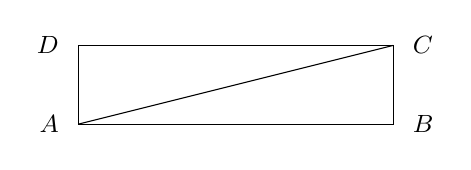
\begin{tikzpicture}[x=10mm,y=10mm,font=\small]
  \draw (1,1) rectangle (5,2);
  \draw (1,1)--(5,2);
  
  \node [label={[name=label node]left:$A$}] at (1,1) {};
  \node [label={[name=label node]left:$D$}] at (1,2) {};
  \node [label={[name=label node]right:$C$}] at (5,2) {};
  \node [label={[name=label node]right:$B$}] at (5,1) {};

%  \foreach \x in {1,5}
%    \foreach \y in {1,2}
%      \filldraw[fill=black, draw=black]  (\x,\y) circle (1pt);

\end{tikzpicture}

\end{center}

\emph{Dati}: $2p = 2(\overline{AB}+\overline{BC})= 80\unit{m}$, $\Area = 375\unit{m^2}$.

\emph{Obiettivo}: $\overline{AC}$.

\begin{soluzione}

$\overline{AC} = \sqrt{\overline{AB}^{2} + \overline{BC}^{2}}$ per il teorema di Pitagora applicato al triangolo $ABC$ retto in $B$.

Sono incognite le misura dei lati, quindi poniamo $\overline{AB}=x$ e $\overline {BC}=y$ con $x>0$ e $y>0$.

Il problema si formalizza con il sistema:
$\left\{ \begin{array}{l} x + y = 40 \\x \cdot y = 375 \end{array}\right.$
che esprime la ricerca di due numeri nota la loro somma $40$ e il loro prodotto $375$. I numeri richiesti sono le soluzioni reali positive dell'equazione $t^{2} - 40 t + 375 = 0$ e precisamente $t_{1} = 15 \vee t_{2} = 25$.

Per come abbiamo disegnato la figura abbiamo quindi: $\overline{AB} = 25\unit{m}$ e $\overline{BC} = 15\unit{m}$, da cui $\overline{AC} = \sqrt{\overline{AB}^{2} + \overline{BC}^{2}} =\sqrt{850} = 5 \sqrt{34}\unit{m}$.
\end{soluzione}

\vspazio\ovalbox{\risolvii \ref{ese:3.91}, \ref{ese:3.92}, \ref{ese:3.93}}

\section{Scomposizione del trinomio di secondo grado}

Si consideri il trinomio di secondo grado: $a x^{2} + b x + c$ e sia $a x^{2} + b x + c = 0$ (con $\Delta \geq 0$) l'equazione associata a tale trinomio. Effettuiamo le seguenti operazioni:
\begin{itemize*}
\item si mette in evidenza $a$: $a x^{2} + b x + c = a \left( x^{2} + \frac{b}{a} x + \frac{c}{a} \right)$;
\item si sostituiscono le relazioni trovate nel precedente paragrafo riguardo la somma e il prodotto delle soluzioni $x_{1}$ e $x_{2}$: $a \left( x^{2} + \frac{b}{a} x + \frac{c}{a} \right) = a \left[x^{2} - ( x_{1} + x_{2} ) x + x_{1} \cdot x_{2} \right]$;
\item si svolgono i calcoli nella parentesi quadra:
\[a \left[ x^{2} - ( x_{1} + x_{2} ) x + x_{1} x_{2}\right] = a\left[ x^{2} - x_{1} x - x_{2} x + x_{1} x_{2}\right];\]
\item si effettua il raccoglimento parziale e si ottiene:
\[a \left[x^{2} - x_{1} x - x_{2} x + x_{1} x_{2}\right] = a \left[ {x \left(x - x_{1} \right) - x_{2} \left( x - x_{1}\right)}\right] = a \left( x - x_{1} \right) \left( x - x_{2} \right).\]
\end{itemize*}

Sulla base del segno di $\Delta$ è possibile distinguere i casi illustrati in tabella:
\begin{center}
\begin{tabular*}{.9\textwidth}{@{\extracolsep{\fill}}*{3}{l}}
\toprule
Discriminante & Soluzioni & Scomposizione \\
\midrule
Caso I:\quad $\Delta > 0$ & $x_{1} \neq x_{2}$ & $a x^{2} + b x + c=a ( x - x_{1} ) ( x - x_{2} )$\\
Caso II:\quad $\Delta = 0$ & $x_{1} = x_{2}$ & $a x^{2} + b x + c=a ( x - x_{1} )^{2}$ \\
Caso III:\quad $\Delta < 0$ & $x_{1}$, $x_{2} \notin \insR$ & $a x^{2} + b x + c$\quad è irriducibile \\
\bottomrule
\end{tabular*}
\end{center}
\begin{exrig}
\begin{esempio}
Scomporre in fattori i seguenti trinomi.
\begin{itemize*}
\item $x^{2} - 5 x + 6$.

Calcolo le soluzioni dell'equazione $x^{2} - 5 x + 6 = 0$. Si ha $x_{1\text{,}2} = \dfrac{5 \pm \sqrt{25 - 24}}{2}$, cioè $x_{1} = 2 \vee x_{2} = 3$. Applicando la formula ottenuta nel caso I si ha: \[x^{2} - 5 x + 6=( x - 2 ) ( x - 3 ).\]
\item $x^{2} - 12 x + 36$.

Poiché $\Delta = 144 - 144 = 0$ il trinomio è un quadrato di un binomio e applicando la formula ottenuta nel caso II si ha: $x^{2} - 12 x + 36=( x - 6 )^{2}$.
\item $2 x^{2} + 3 x + 5$.

Essendo $\Delta=9 - 40=-31$, il trinomio è irriducibile.
\item $- 5 x^{2} + 2 x + 1$.

Calcolo le radici dell'equazione associata $- 5 x^{2} + 2 x + 1 = 0$: $x_{1\text{,}2} = \frac{- 2 \pm \sqrt{24}}{- 10} = \frac{1 \pm \sqrt{6}}{5}$ quindi $x_{1} = \frac{1 - \sqrt{6}}{5} \vee x_{2} = \frac{1 + \sqrt{6}}{5}$ e scrivo la scomposizione: \[- 5 x^{2} + 2 x + 1=- 5 \left( x - \frac{1 - \sqrt{6}}{5} \right) \left( x - \frac{1 + \sqrt{6}}{5} \right).\]
\end{itemize*}
\end{esempio}

\begin{esempio}
Scrivere un'equazione di secondo grado che ammetta le seguenti soluzioni $x_{1} = \frac{1}{2}$ e $x_{2} = 3$.

Per quanto visto nel paragrafo, si ha
\[\left(x-\frac{1}{2} \right) \left(x + 3 \right)=0 \Rightarrow x^{2} + 3 x-\frac{1}{2} x - \frac{3}{2}=0 \Rightarrow x^{2} + 5 x - \frac{3}{2}=0 \Rightarrow 2 x^{2} + 5 x-3=0.\]
%\begin{align*}
%&\left(x-\frac{1}{2} \right) \left(x + 3 \right)=0\\
%\Rightarrow\: & x^{2} + 3 x-\frac{1}{2} x - \frac{3}{2}=0\\
%\Rightarrow\: & x^{2} + 5 x - \frac{3}{2}=0\\
%\Rightarrow\: & 2 x^{2} + 5 x-3=0
%\end{align*}
\end{esempio}
\end{exrig}

\osservazione
Si vuole scomporre in fattori il trinomio $m = 4 x^{2} + 2 x - 6$, avente tutti i coefficienti pari. Anche se osserviamo che tutti i suoi coefficienti sono pari, non possiamo dividire per due, non essendo un'equazione. Il polinomio $m = 2 x^{2} + x - 3$ è diverso da quello assegnato, mentre le equazioni associate all'uno e all'altro sono equivalenti. Nel procedere alla scomposizione, una volta trovate le radici, per ottenere le quali possiamo anche usare l'equazione equivalente $2 x^{2} + x - 3 = 0$, è necessario moltiplicare per $a$. Quindi, in questo caso le radici sono $x_{1} = - \frac{3}{2} \vee x_{2} = 1$ e pertanto il trinomio assegnato si scompone come: $4 x^{2} + 2 x - 6 = 4 \left( x + \frac{3}{2} \right) ( x - 1)$.

\vspazio\ovalbox{\risolvii \ref{ese:3.94}, \ref{ese:3.95}, \ref{ese:3.96}}

\section{Regola di Cartesio}

Se in un'equazione di secondo grado i coefficienti sono tutti diversi da zero e il discriminante è non negativo, è possibile avere delle informazioni sui
segni delle soluzioni senza calcolarle esplicitamente.

\pagebreak
In un'equazione $a x^{2} + b x + c = 0$, dove i coefficienti sono tutti non nulli, le coppie di coefficienti $(a;b)$ e~$(b;c)$ sono dette coppie di \emph{coefficienti consecutivi}. Una coppia di coefficienti consecutivi presenta:
\begin{itemize*}
\item una \emph{permanenza} se i coefficienti hanno lo stesso segno;
\item una \emph{variazione} se i coefficienti hanno segni diversi.
\end{itemize*}

\begin{exrig}
\begin{esempio}
Determinare le variazioni e le permanenze nelle seguenti equazioni:
\begin{center}
\begin{tabular*}{.9\textwidth}{@{\extracolsep{\fill}}*{10}{c}}
\toprule
Equazione & $a$ & & & & $b$ & & & & $c$ \\
\midrule
$2 x^{2} - 3 x - 1$ & $+$ & $\rightarrow$ & variazione & $\leftarrow$ & $-$ & $\rightarrow$ & permanenza & $\leftarrow$ & $-$\\
$- x^{2} - 3 x - 1$ & $-$ & $\rightarrow$ & permanenza & $\leftarrow$ & $-$ & $\rightarrow$ & permanenza & $\leftarrow$ & $-$\\
$- 3 x^{2} + 4 x - 1$ & $-$ & $\rightarrow$ & variazione & $\leftarrow$ & $+$ & $\rightarrow$ & variazione & $\leftarrow$ & $-$\\
$2 x^{2} + x - 1$ & $+$ & $\rightarrow$ & permanenza & $\leftarrow$ & $+$ & $\rightarrow$ & variazione & $\leftarrow$ & $-$\\
\end{tabular*}
\end{center}

\end{esempio}
\end{exrig}

\begin{teorema}[di Cartesio]
In un'equazione di secondo grado $a x^{2} + b x + c = 0$ con $a$, $b$, $c \neq 0$ e $\Delta \geq 0$, il numero di radici positive è uguale al numero di variazioni presenti nelle coppie di coefficienti consecutivi. Se vi è una sola variazione, le radici sono discordi e il valore assoluto maggiore è quello della radice positiva se la variazione è nella coppia $(a;b)$, mentre è della radice negativa se la variazione è nella coppia $(b;c)$.
\end{teorema}

\begin{exrig}
\begin{esempio}
Determinare il segno delle soluzioni dell'equazione $x^2 + 2 x - 3 = 0$ senza risolverla.

L'equazione $x^2 + 2 x - 3 = 0$ ha soluzioni reali in quanto $\Delta = 16 > 0$. Dal momento che vi è una sola variazione, quella della coppia $(b;c)$, l'equazione ha radici discordi e il valore assoluto maggiore è quello della radice negativa.

Dimostriamo quanto è stato affermato tenendo presente che $x_{1} + x_{2} = - \frac{b}{a}$ e $x_{1}\cdot x_{2} = \frac{c}{a}$; nell'equazione proposta si ha:
$x_{1} + x_{2} = - 2$ e $x_{1} \cdot x_{2} = - 3$ dunque prodotto negativo e somma negativa. Il prodotto di due numeri è negativo quando i fattori sono discordi, quindi una soluzione è positiva e una è negativa. Chiamiamo $x_1$ la soluzione negativa e $x_2$ la soluzione positiva, poiché $x_{1} + x_{2} = - 2 < 0$ deduciamo che in valore assoluto è più grande il numero negativo, cioè $\valass{x_{1}} > \valass{x_{2}}$.
\end{esempio}

\begin{esempio}
Determinare il segno delle soluzioni delle seguenti equazioni senza risolverle.
\begin{itemize}
	\item $2 x^{2} - 6 x - 56 = 0$. L'equazione ha soluzioni reali in quanto $\Delta = 484 > 0$; dal momento che vi è una sola variazione le radici sono discordi
	e il valore assoluto maggiore è quello della radice positiva poiché che la variazione è nella coppia $(a;b)$.
	\item $-3 x^{2} - 24 x - 21 = 0$. L'equazione ha soluzioni reali in quanto $\Delta = 324 > 0$; dal momento che non vi sono variazioni, l'equazione ha due radici negative.
	\item $x^{2} - 10 x + 25 = 0$. L'equazione ha due soluzioni coincidenti in quanto $\Delta = 0$; dal momento che vi sono due variazioni, le due radici coincidenti sono positive.
\end{itemize}
\end{esempio}
\end{exrig}
\vspazio\ovalbox{\risolvi \ref{ese:3.97}}

\section{Equazioni parametriche}

\begin{definizione}

Si definisce \emph{parametrica} un'equazione i cui coefficienti dipendono da un parametro.
\end{definizione}

L'equazione $3 x^{2} + ( k - 1 ) x + 2 - 3 k= 0$ è parametrica di secondo grado nell'incognita $x$; i suoi coefficienti dipendono dal valore del parametro $k$ e quindi la natura e il segno delle sue soluzioni dipendono da $k$.

In molti problemi di applicazione della matematica in situazioni reali in cui compare un parametro, non interessa tanto determinare le soluzioni dell'equazione che formalizza il problema, quanto sapere se le soluzioni hanno determinate caratteristiche.
Sappiamo che attraverso i coefficienti di un'equazione di secondo grado si possono determinare alcune relazioni tra le sue soluzioni:
\begin{itemize*}
\item soluzioni reali se $\Delta = b^{2} - 4 a c \geq 0$; reali coincidenti se $\Delta = 0$, reali distinte se $\Delta > 0$;
\item la somma delle soluzioni è $x_{1} + x_{2} = - \dfrac{b}{a}$;
\item il prodotto delle soluzioni è $x_{1} \cdot x_{2} = \dfrac{c}{a}$.
\end{itemize*}

Nell'equazione $3 x^{2} + ( k - 1 ) x + 2 - 3 k = 0$ si ha $\Delta = ( k - 1 )^{2} - 12 ( 2 - 3 k )$ dipendente dal parametro $k$.
Dall'analisi del $\Delta$ si potranno dedurre quali condizioni deve verificare $k$ affinché esistano soluzioni reali. Analizzando somma e prodotto
$x_{1} + x_{2} = - \frac{( k - 1 )}{3}$ e $x_{1} \cdot x_{2} =\frac{( 2 - 3 k )}{3}$ potremo stabilire il segno ed altre caratteristiche delle soluzioni.

\begin{exrig}
\begin{esempio}
Data l'equazione $( k + 1 ) x^{2} + ( 2 k + 3 ) x + k = 0$, stabilire per quale valore di $k$
\begin{enumeratea}
\item l'equazione si riduce al primo grado;
\item l'equazione ammette soluzioni reali distinguendo i casi ``soluzioni coincidenti'' e ``soluzioni distinte'';
\item la somma delle soluzioni sia nulla, determinando in tal caso le soluzioni.
\end{enumeratea}
\emph{Svolgimento}
\begin{enumeratea}
\item l'equazione diventa di primo grado se il coefficiente $a$ si annulla, cioè se $k + 1 = 0$ quindi $k = - 1$. In tal caso si ha una sola soluzione reale $ x=1 $;
\item studiamo il segno del discriminante: $\Delta = ( 2 k + 3 )^{2} - 4 k ( k + 1 ) \geq 0$ da cui ricaviamo 
\[4 k^{2} + 12 k + 9 - 4 k^{2} - 4 k \geq 0 \:\Rightarrow\: 8 k + 9 \geq 0.\] 
Pertanto se $k = - \frac{9}{8}$ le soluzioni sono coincidenti, se $k > - \frac{9}{8}$ le soluzioni sono reali distinte, se invece $ k<-\frac{9}{8} $ non ci sono soluzioni reali;
\item dalla formula della somma delle soluzioni ricaviamo $x_{1} + x_{2} = - \frac{( 2 k + 3 )}{( k + 1 )}$ e quindi la somma sarà nulla se $2 k + 3 = 0 \:\Rightarrow\: k = - \frac{3}{2}$. Poiché $- \frac{3}{2} < - \frac{9}{8}$, per $k = - \frac{3}{2}$ non ci sono soluzioni reali, infatti sostituendolo nell'equazione quest'ultima diventa $ x^2+3=0 \Rightarrow x^2=-3$ impossibile!
\end{enumeratea}
\end{esempio}
\end{exrig}
\vspazio\ovalbox{\risolvii \ref{ese:3.98}, \ref{ese:3.99}, \ref{ese:3.100}, \ref{ese:3.101}, \ref{ese:3.102}, \ref{ese:3.103}, \ref{ese:3.104}, \ref{ese:3.105}, \ref{ese:3.106}, \ref{ese:3.107}, \ref{ese:3.108},}

\vspazio\ovalbox{ \ref{ese:3.109},\ref{ese:3.110}, \ref{ese:3.111}, \ref{ese:3.112}, \ref{ese:3.113}, \ref{ese:3.114}, \ref{ese:3.115}, \ref{ese:3.116}, \ref{ese:3.117}, \ref{ese:3.118}, \ref{ese:3.119}, \ref{ese:3.120}, \ref{ese:3.121}, \ref{ese:3.122}}

\section{Problemi di secondo grado in una incognita}

 \epigraph{La risoluzione dei problemi [\ldots] serve ad acuire l'ingegno e a dargli la facoltà di penetrare
 l'intera ragione di tutte le cose.}{{\scshape{R. Descartes}}}

Sappiamo che nel corso degli studi o nell'attività lavorativa possono presentarsi problemi di diversa natura: di tipo economico, scientifico, sociale; possono riguardare insiemi numerici o figure geometriche. La matematica ci può aiutare a risolvere i problemi quando essi possono essere tradotti in ``forma matematica'', quando cioè è possibile trascrivere in simboli le relazioni che intercorrono tra le grandezze presenti nel problema e quando si può costruire, tramite queste relazioni, un modello matematico che ci permetta di raggiungere la soluzione al quesito.

Affronteremo problemi di tipo algebrico o geometrico, che potranno essere formalizzati attraverso equazioni di secondo grado in una sola incognita.
Teniamo presente, prima di buttarci nella risoluzione del problema, alcuni passi che ci aiuteranno a costruire il modello matematico:
\begin{itemize}
\item la lettura ``attenta'' del testo al fine di individuare l'ambiente del problema, le parole chiave, i dati e le informazioni implicite, l'obiettivo;
\item la scelta della grandezza incognita del problema, la descrizione dell'insieme in cui si ricerca il suo valore, le condizioni che devono essere soddisfatte dall'incognita;
\item la traduzione in ``forma matematica'' delle relazioni che intercorrono tra i dati e l'obiettivo, cioè l'individuazione del modello matematico (equazione risolvente).
\end{itemize}
Dopo aver risolto l'equazione occorre confrontare la soluzione trovata con le condizioni poste dal problema.

\begin{problema}
Nel triangolo rettangolo $ABC$ rettangolo in $C$, l'ipotenusa $AB$ supera il cateto maggiore $BC$ di $2\unit{m}$; la differenza tra i cateti è $23\unit{m}$. Determinare la misura del perimetro e l'area del triangolo.
\end{problema}

\begin{multicols}{3}
\emph{Dati}

$\overline {AB} = \overline {BC} + 2$;

$\overline {BC} - \overline {AC} = 23$;

$A \widehat {C} B = 90\grado$.

\emph{Obiettivo}

$2p$;

Area.

 % (c) 2013 Claudio Carboncini - claudio.carboncini@gmail.com
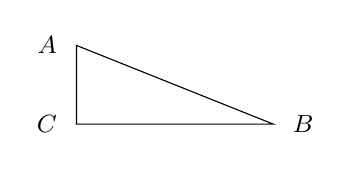
\begin{tikzpicture}[x=10mm,y=10mm,font=\small]

  \draw (1,1) -- (1,2) -- (3.5,1) -- cycle;
  \node [label={[name=label node]left:$A$}] at (1,2) {};
  \node [label={[name=label node]right:$B$}] at (3.5,1) {};
  \node [label={[name=label node]left:$C$}] at (1,1) {};

\end{tikzpicture}

\end{multicols}

\begin{soluzione}

Osserva che $2p = \overline {AB} + \overline {BC} + \overline {AC}$ e $\Area =\frac{\overline {BC} \cdot \overline {AC}}{2}$.
Ponendo $\overline {BC} = x$, si ha $\overline {AB} = x + 2$~~e~~$\overline{AC} = x - 23$~~con
$\left\{\begin{array}{l} x > 0 \text{ essendo misura di un segmento} \\x >23 \text{ poiché } \overline {AC} \text{ deve essere positiva}
\end{array}\right.$.

Essendo rettangolo, i lati del triangolo sono legati dal teorema di Pitagora
quindi si deve verificare: $\overline {AB}^{2}= \overline {AC}^{2} + \overline {BC}^{2}\:\Rightarrow\: ( x + 2 )^{2} = ( x - 23 )^{2} + x^{2}$. Sviluppando i calcoli si ottiene l'equazione risolvente di secondo grado, in forma canonica: $x^{2} - 50 x + 525 = 0$ con $\Delta = 400$. L'equazione è quindi determinata pertanto esistono due soluzioni reali distinte: $x_{1} = 15 \vee x_{2} = 35$ entrambe positive. Ai fini del problema $x_{1} = 15$ non è accettabile, quindi il problema ha una sola soluzione: $\overline {BC} = 35 \:\Rightarrow\: \overline {AB} = 37$ e $\overline {AC} = 12$. Conclusione: $2p = 35 + 37 + 12 = 84\unit{m}$~~e~~$\Area = 210\unit{m^{2}}$.
\end{soluzione}

\begin{problema}
Un padre aveva $26$ anni alla nascita del figlio; moltiplicando le età attuali del padre e del figlio si ottiene il triplo del quadrato dell'età del figlio; calcolare le due età.
\end{problema}

Indichiamo con $p$ l'età attuale del padre e con $f$ l'età attuale del figlio.

\emph{Dati}: $p = f + 26$~~e~~$p \cdot f = 3 f^{2}$.

\emph{Obiettivo}: $f$, $p$.

\begin{soluzione}
I dati permettono di impostare la relazione $(f + 26) \cdot f = 3 \cdot f^{2}$ che esprime il legame tra le età di oggi del padre e del figlio; siamo di
fronte ad un'equazione di secondo grado nell'incognita $f$. La soluzione dell'equazione deve essere espressa da un numero positivo poiché esprime l'età.
Risolviamo l'equazione $2 f^{2} - 26 f = 0$ le cui soluzioni sono $f_{1} = 0 \vee f_{2} = 13$. Per le condizioni poste la soluzione del problema è
$f = 13$. Quindi oggi il figlio ha $13$ anni e, di conseguenza, il padre $39$.
\end{soluzione}

\begin{problema}
Il trapezio isoscele $ABCD$ è inscritto in una semicirconferenza di diametro $AB$ di misura $25\unit{cm}$; determina le misure dei lati del trapezio sapendo che il
suo perimetro è $62\unit{cm}$.
\end{problema}

\begin{multicols}{2}
\emph{Dati}

$\overline {AB} = 25$;~~$2p = 62$;

$AB \parallel CD$;~~$\overline {AD} = \overline {BC}$.

\emph{Obiettivo}

$\overline {CD}$;~~$ \overline {BC}$.

 % (c) 2013 Claudio Carboncini - claudio.carboncini@gmail.com
\begin{tikzpicture}[x=10mm,y=10mm,font=\small]
  \coordinate(a) at (-2.5,0);
  \coordinate(d) at (120:2.5);
  \coordinate(e) at (90:2.5);
  \coordinate(c) at (60:2.5);
  \coordinate(b) at (2.5,0);
  \coordinate (h) at ($(a)!(c)!(b)$);%trova le coordinate della proiezione di c su a--b
  \draw (-2.5,0) arc (180:0:2.5) -- cycle;% semicirconferenza e diametro
  \draw (a) -- (d) -- (c) -- (b);%disegna il trapezio
  \draw [dotted] (e) -- (0,0);%da E a O
  \draw [dotted] (c) -- (h);% c--h
  \draw [dotted] (e) -- (b);% e--b
  \node [label={[name=label node]below left:$A$}] at (a) {};
  \node [label={[name=label node]below right:$B$}] at (b) {};
  \node [label={[name=label node]above right:$C$}] at (c) {};
  \node [label={[name=label node]above left:$D$}] at (d) {};
  \node [label={[name=label node]above:$E$}] at (e) {};
  \node [label={[name=label node]below:$H$}] at (h) {};
  \filldraw[fill=black, draw=black]  (a) circle (1pt);
  \filldraw[fill=black, draw=black]  (b) circle (1pt);
  \filldraw[fill=black, draw=black]  (c) circle (1pt);
  \filldraw[fill=black, draw=black]  (d) circle (1pt);
  \filldraw[fill=black, draw=black]  (h) circle (1pt);
  \filldraw[fill=black, draw=black]  (e) circle (1pt);

\end{tikzpicture}

\end{multicols}

\begin{soluzione}
$\overline {AB} + \overline {CD} + 2 \overline {BC} = 62$; fissiamo come incognita $\overline {BC} = x$.
Determiniamo le condizioni sull'incognita: dovrà essere $x > 0$ poiché rappresenta la misura di un segmento e inoltre affinché esista
realmente il trapezio isoscele il punto $C$ non deve coincidere con il punto medio $E$ dell'arco $CD$ cioè $ CB<EB $, quindi $x < \dfrac{25}{2} \sqrt{2}$.

Tracciata l'altezza $CH$ ($H \in AB$) si ha $\overline {CD} = \overline {AB} - 2 \overline {HB}$ e per il 1° teorema di Euclide\footnote{in ogni triangolo rettangolo ciascun cateto è medio proporzionale tra l'ipotenusa e la proiezione del cateto stesso sull'ipotenusa.} sul triangolo~$ACB$, rettangolo in
$C$ (poiché insiste su una semicirconferenza con diametro $AB$), $\overline {HB}: \overline {CB} = \overline {CB} : \overline{AB}$; determiniamo quindi la misura di $HB$ in funzione dell'incognita fissata:
$\overline {HB} = \dfrac{x^{2}}{25}$ da cui $\overline{CD} = 25 - \dfrac{2 x^{2}}{25}$.

Costruiamo l'equazione risolvente: $25 + 2 x + 25 - \dfrac{2 x^{2}}{25} = 62 \:\Rightarrow\: x^{2} - 25 x + 150 = 0$ che ha soluzioni $x_{1} = 10 \vee x_{2} = 15$, entrambe accettabili. Si hanno dunque due trapezi inscritti che risolvono il problema. Poiché $\overline{CD}= 2p-\overline{AB}-2\overline{BC}$ si ha $\overline{CD}=62-25-10=27\unit{cm}$ o $\overline{CD}=62-25-15=22\unit{cm}$.
\begin{center}
 % (c) 2013 Claudio Carboncini - claudio.carboncini@gmail.com
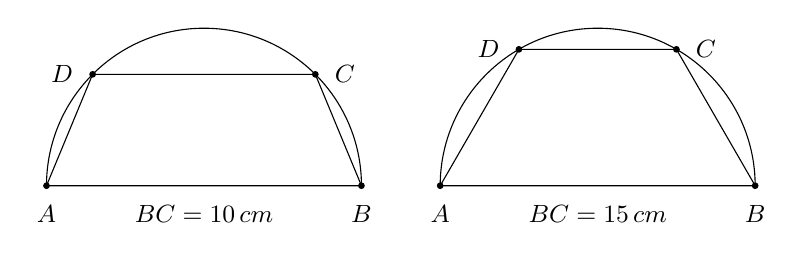
\begin{tikzpicture}[x=10mm,y=10mm,font=\small]
  \coordinate(a) at (-2,0);
  \coordinate(d) at (135:2);
  \coordinate(c) at (45:2);
  \coordinate(b) at (2,0);
  \coordinate(a1) at (3,0);
  \coordinate(d1) at (4,1.732);
  \coordinate(c1) at (6,1.732);
  \coordinate(b1) at (7,0);
  \coordinate(t) at (0,0);
  \coordinate(t1) at (5,0);
  \draw (-2,0) arc (180:0:2) -- cycle;% semicirconferenza e diametro primo trapezio
  \draw (3,0) arc (180:0:2) -- cycle;% semicirconferenza e diametro secondo trapezio
  \draw (a) -- (d) -- (c) -- (b);%disegna il trapezio
  \draw (a1) -- (d1) -- (c1) -- (b1);%disegna il secondo trapezio
  \node [label={[name=label node]below:$A$}] at (a) {};
  \node [label={[name=label node]below:$B$}] at (b) {};
  \node [label={[name=label node]right:$C$}] at (c) {};
  \node [label={[name=label node]left:$D$}] at (d) {};
  \node [label={[name=label node]below:$BC=10\,  cm$}] at (t) {};
  \node [label={[name=label node]below:$A$}] at (a1) {};
  \node [label={[name=label node]below:$B$}] at (b1) {};
  \node [label={[name=label node]right:$C$}] at (c1) {};
  \node [label={[name=label node]left:$D$}] at (d1) {};
  \node [label={[name=label node]below:$BC=15\,  cm$}] at (t1) {};
  \filldraw[fill=black, draw=black]  (a) circle (1pt);
  \filldraw[fill=black, draw=black]  (b) circle (1pt);
  \filldraw[fill=black, draw=black]  (c) circle (1pt);
  \filldraw[fill=black, draw=black]  (d) circle (1pt);
  \filldraw[fill=black, draw=black]  (a1) circle (1pt);
  \filldraw[fill=black, draw=black]  (b1) circle (1pt);
  \filldraw[fill=black, draw=black]  (c1) circle (1pt);
  \filldraw[fill=black, draw=black]  (d1) circle (1pt);

\end{tikzpicture}

\end{center}
\end{soluzione}

\begin{problema}
Un capitale di \officialeuro~$\np{25000}$ viene depositato in banca a un tasso di interesse annuo $c$. Gli interessi maturati durante il primo anno non vengono ritirati.
Nell'anno seguente si investono sia il capitale sia gli interessi maturati a un tasso di interesse annuo aumentato dello $\np{0,5}\%$. Alla fine dei due anni si ritira
la somma di \officialeuro~$\np{26291,10}$. Calcola i tassi di interesse praticati dalla banca.
\end{problema}
Assumiamo come incognita $c$ il tasso di interesse praticato il primo anno, espresso come numero decimale e
non in forma percentuale. Il tasso praticato nel secondo anno sarà $c+\np{0,005}$.

\begin{soluzione}
Alla fine del primo anno in banca si hanno tra capitale e interessi \[\np{25000} + \np{25000} \cdot c = \np{25000} ( 1 + c ).\] Nel secondo anno il tasso praticato è $c+\np{0,005}$ che va applicato alla somma $\np{25000}(1+c)$. Si ottiene quindi l'equazione \[\np{25000} ( 1 + c ) ( 1 + c + \np{0,005} ) = \np{26291,10}.\]
Moltiplicando le parentesi tonde si ha $\np{25000} ( \np{1,005} + c + \np{1,005} c + c^{2} ) = \np{26291,10}$ e poi dividendo per $\np{25000}$ e ordinando otteniamo
$c^{2} + \np{2,005} c - \np{0,046644}=0$ con soluzioni
\[c_{1\text{,}2} = \dfrac{- \np{2,005} \pm \sqrt{\np{4,020025} + \np{0,186576}}}{2} = \dfrac{\np{-2,005} \pm \np{2,051}}{2}\:\Rightarrow\: c_{1} = \np{-2,028} \vee c_{2} = \np{0,023}.\]
La soluzione $c_1$ è negativa e pertanto non accettabile. La risposta al problema è $\np{0,023}$ cioè $\np{2,3}\%$ il primo anno e quindi $\np{2,8}\%$ il secondo anno.
\end{soluzione}

\vspazio\ovalbox{\risolvii \ref{ese:3.123}, \ref{ese:3.124}, \ref{ese:3.125}, \ref{ese:3.126}, \ref{ese:3.127}, \ref{ese:3.128}, \ref{ese:3.129}, \ref{ese:3.130}, \ref{ese:3.131}, \ref{ese:3.132},}

\vspazio\ovalbox{ \ref{ese:3.133}, \ref{ese:3.134}, \ref{ese:3.135}, \ref{ese:3.136}, \ref{ese:3.137}, \ref{ese:3.138}, \ref{ese:3.139}, \ref{ese:3.140}, \ref{ese:3.141}, \ref{ese:3.142}, \ref{ese:3.143}, \ref{ese:3.144}, \ref{ese:3.145}, }

\vspazio\ovalbox{\ref{ese:3.146}, \ref{ese:3.147},\ref{ese:3.148}, \ref{ese:3.149}, \ref{ese:3.150}, \ref{ese:3.151}, \ref{ese:3.152}, \ref{ese:3.153}, \ref{ese:3.154}, \ref{ese:3.155}, \ref{ese:3.156}, \ref{ese:3.157}, \ref{ese:3.158}, }

\vspazio\ovalbox{\ref{ese:3.162}, \ref{ese:3.163}, \ref{ese:3.164}, \ref{ese:3.165}, \ref{ese:3.166}, \ref{ese:3.167}, \ref{ese:3.168}, \ref{ese:3.169},\ref{ese:3.159}, \ref{ese:3.160}, \ref{ese:3.161},}

\subsection{Problemi con un parametro}

I problemi che abbiamo proposto sono caratterizzati da dati numerici e di conseguenza le soluzioni numeriche dell'equazione risolvente sono facilmente
confrontabili con le condizioni poste sull'incognita. Abbiamo anche visto che le soluzioni dell'equazione non sempre sono soluzioni del problema e
può anche succedere che il problema abbia due soluzioni.

Affrontiamo ora un problema letterale, nel quale alcuni dati sono espressi da lettere. In questi problemi dovremo rispettare le condizioni poste sull'incognita, ma anche analizzare per quali valori della lettera il problema ammette soluzioni reali. Dovremo quindi procedere con la discussione dell'equazione parametrica risolvente per stabilire se il problema letterale ammette soluzioni.

\begin{problema}
Sul lato $ a $ dell'angolo $ a \widehat{V} b $ di $ 60\grado $ si fissano i punti $ A $ e $ B $ tali che $ \overline{VA} = 2 k $ e $ \overline {VB} = 8 k $.
Determina sul lato $ b $ un punto $ P $ in modo che il rapporto tra $\overline{PB}$ e $\overline{PA}$ sia $2$.
\end{problema}

\begin{multicols}{2}
\emph{Dati}

$a \widehat{V} b = 60\grado$;

$\overline {VA} = 2 k; \;
 \overline {VB} = 8 k $.

\emph{Obiettivo}

$P \in b \text{ tale che } \dfrac{\overline{PB}}{\overline{PA}} = 2$.
\begin{center}
 % (c) 2013 Claudio Carboncini - claudio.carboncini@gmail.com
\begin{tikzpicture}[x=10mm,y=10mm,font=\small]

  \coordinate(v) at (0,0);%il vertice dell'angolo
  \coordinate(a) at (60:4);%la retta a
  \coordinate(b) at (4,0);%la retta b
  \coordinate(a1) at (60:1.8);%il punto A
  \coordinate(b1) at (60:3.2);%il punto B
  \coordinate(p) at (3.2,0);%il punto P
  \coordinate (m) at ($(v)!(b1)!(p)$);%trova le coordinate della proiezione di b su v--p
  \coordinate (n) at ($(v)!(a1)!(p)$);%trova le coordinate della proiezione di b su v--p
  \draw (a) -- (v)  -- (b);%disegna l'angolo
  \draw [dotted] (b1) -- (p);%disegna il segmento b--p
  \draw [dotted] (a1) -- (p);%disegna il segmento a--p
  \draw [dotted] (a1) -- (n);%perpendicolare da A a b
  \draw [dotted] (b1) -- (m);%perpendicolare da B a b
  \node [label={[name=label node]left:$V$}] at (v) {};
  \node [label={[name=label node]left:$A$}] at (a1) {};
  \node [label={[name=label node]left:$B$}] at (b1) {};
  \node [label={[name=label node]left:$a$}] at (a) {};
  \node [label={[name=label node]below:$P$}] at (p) {};
  \node [label={[name=label node]below:$M$}] at (m) {};
  \node [label={[name=label node]below:$N$}] at (n) {};
  \node [label={[name=label node]above:$b$}] at (b) {};
  \filldraw[fill=black, draw=black]  (a1) circle (1pt);
  \filldraw[fill=black, draw=black]  (b1) circle (1pt);
  \filldraw[fill=black, draw=black]  (p) circle (1pt);
  \draw [<->] (3mm,0) arc (0:60:3mm);
\end{tikzpicture}

\end{center}

\end{multicols}
\emph{Osservazione preliminare}: le misure dei segmenti $ VA $ e $ VB $ sono espresse in forma letterale, affinché il problema abbia significato deve essere
$k > 0$.

\begin{soluzione}
La posizione del punto $ P $ sul lato $ b $ sarà individuata dalla distanza di $ P $ da $ V $: poniamo quindi $\overline {VP} = x$ con $x > 0$ e determiniamo
$\overline {PB}$ e $\overline {PA}$ in funzione di $ x $ per poter sfruttare la richiesta contenuta nell'obiettivo come equazione risolvente.

Sia $ M $ il piede della perpendicolare da $ B $ al lato $ b $; nel triangolo rettangolo $ PMB $ si ha $\overline {PB}^{2} = \overline {BM}^{2} + \overline {PM}^{2}$ (*) per il teorema di Pitagora. Nel triangolo $ BVM $, rettangolo in $ M $ con l'angolo $ V $ di $ 60\grado $ si ha $\overline {BM} = \frac{1}{2} \overline {BV} \cdot \sqrt{3} = 4 k\cdot \sqrt{3}$; $\overline {PM} = \overline {VP} - \overline {VM}$ e $\overline {VM} = \frac{1}{2} \overline {VB} = 4 k$; per quanto detto sul triangolo $ BVM $, si ha che $\overline {PM} = x - 4 k$; sostituendo in (*) si ottiene \[\overline {PB}^{2} = 48 k^{2} + ( x - 4 k )^{2}.\]

Sia $ N $ il piede della perpendicolare da $ A $ al lato $ b $; nel triangolo rettangolo $ PNA $, con analogo ragionamento otteniamo: $\overline {PA}^{2} = \overline {AN}^{2} + \overline {PN}^{2}$ (**) per il teorema di Pitagora. Nel triangolo $ AVN $, rettangolo in $ N $ con l'angolo $ V $ di $ 60\grado $, si ha
$\overline {AN} = \frac{1}{2} \overline {AV} \cdot \sqrt{3} = k \cdot \sqrt{3}$; $ \overline {VN} = \frac{1}{2} \overline {AV} = k$ e $\overline {PN} = \overline {VP} - \overline {VN} = x - k$; sostituendo in (**) si ottiene \[\overline {PA}^{2} = 3 k^{2} + ( x - k )^{2}.\]
\pagebreak

Determiniamo l'equazione risolvente ricordando che il rapporto tra due segmenti è uguale al rapporto tra le rispettive misure ed elevando al quadrato
si ha $\frac{\overline {PB}^{2}}{\overline {PA}^{2}} = 4$. Sostituendo quanto trovato si ottiene l'equazione $48 k^{2} + ( x - 4 k )^{2} = 4 \cdot \left[ 3 k^{2} + ( x - k )^{2} \right]$ da cui $x^{2} = 16 k^{2}$.

Si tratta di un'equazione di secondo grado pura avente due soluzioni reali opposte, essendo il secondo membro positivo. Quindi $x_{1} = -4 k$ e $x_2=4 k$; per le condizioni poste solo $ x_2 $ è accettabile.

Con quale punto della figura tracciata inizialmente viene a coincidere il punto $ P $ che risolve il problema?
\end{soluzione}

\vspazio\ovalbox{\risolvii \ref{ese:3.170}, \ref{ese:3.171}, \ref{ese:3.172}, \ref{ese:3.173}, \ref{ese:3.174}, \ref{ese:3.175}, \ref{ese:3.176}, \ref{ese:3.177}, \ref{ese:3.178}}

\newpage
% (c)~2014 Claudio Carboncini - claudio.carboncini@gmail.com
% (c)~2014 Dimitrios Vrettos - d.vrettos@gmail.com
\section{Esercizi}
\subsection{Esercizi dei singoli paragrafi}
\subsection*{3.1 - le equazioni di secondo grado in una incognita}

\begin{esercizio}[\Ast]
 \label{ese:3.1}
Risolvi le seguenti equazioni di secondo grado pure.
\begin{multicols}{3}
 \begin{enumeratea}
 \item~$x^{2}-1 = 0$;
 \item~$x^{2}=\frac{49}{25}$;
 \item~$2x^{2} - 32 = 0$;
 \item~$x^{2}-25=0$;
 \item~$16 x^{2}=1$;
 \item~$3x^{2}+3=0$;
 \item~$x^{2}-9=0$;
 \item~$25=9 x^{2}$;
 \item~$x^{2} - 3 = 0$;
 \item~$x^{2} + 36 = 0$;
 \item~$4 - x^{2} = 0$;
 \item~$x^{2} + 4 = 0$.
 \end{enumeratea}
 \end{multicols}
\end{esercizio}

\begin{esercizio}[\Ast]
\label{ese:3.2}
Risolvi le seguenti equazioni di secondo grado pure.
\begin{multicols}{3}
 \begin{enumeratea}
 \item~$x^{2} = 49$;
 \item~$4 - 9 x^{2} = 0$;
 \item~$5 x^{2} - 3 = 0$;
 \item~$4 x^{2} - 9 = 0$;
 \item~$9 x^{2} - 25 = 0$;
 \item~$6 x^{2} = 0$;
 \item~$2 x^{2} - 1 = 0$;
 \item~$4 x^{2} + 16 = 0$;
 \item~$1 + x^{2} = 50$;
 \item~$3 x^{2} - 1 = 0$;
 \item~$27 x^{2} - 3 = 0$;
 \item~$7 x^{2} = 28$.
 \end{enumeratea}
 \end{multicols}
\end{esercizio}

\begin{esercizio}[\Ast]
 \label{ese:3.3}
Risolvi le seguenti equazioni di secondo grado pure.
\begin{multicols}{3}
 \begin{enumeratea}
 \item~$4 x^{2} - 4 = 0$;
 \item~$5 x^{2} - 125 = 0$;
 \item~$0,04 x^{2} = 1$;
 \item~$x^{2} - 0,01 = 0$;
 \item~$0,5 x^{2} - 4,5 = 0$;
 \item~$0,09 x^{2} = 0,01$;
 \item~$\frac{1}{2} x^{2} - 2 = 0$;
 \item~$x^{2} - \frac{9}{4} = 0$;
 \item~$x^{2} - \frac{1}{6} = 0$;
 \item~$121 x^{2} - \frac{1}{169} = 0$;
 \item~$x^{2} + \frac{9}{4} = 0$;
 \item~$4 \left(x^{2}-\frac{3}{4}\right)= 13$.
 \end{enumeratea}
 \end{multicols}
\end{esercizio}

\begin{esercizio}[\Ast]
 \label{ese:3.4}
Risolvi le seguenti equazioni di secondo grado pure.
\begin{multicols}{2}
 \begin{enumeratea}
 \item~$x^{2} - \sqrt{3} = 0$;
 \item~$- 9 x^{2} = - 1$;
 \item~$4 x^{2} = - 9$;
 \item~$x^{2} + 6 = 42$;
 \item~$5 - 125 x^{2} = 0$;
 \item~$18 - x^{2} = 0$;
 \item~$(x + 3)^{2} = 6 x + 34$;
 \item~$(x + 1)^{2} = 25$;
 \item~$(x - \sqrt{3}) (x + \sqrt{3}) = 13$;
 \item~$(x + \sqrt{2})^{2} = 2 \sqrt{2} x$;
 \item~$(x - 2)^{2} + (1 - x)^{2} = 1 - 6x$;
 \item~$(\sqrt{2} x - \sqrt{3}) (\sqrt{2} x + \sqrt{3}) = 0$.
 \end{enumeratea}
 \end{multicols}
\end{esercizio}

\begin{esercizio}[\Ast]
\label{ese:3.5}
Risolvi le seguenti equazioni di secondo grado spurie.
\begin{multicols}{3}
 \begin{enumeratea}
 \item~$x^{2} - 3 x = 0$;
 \item~$3 x^{2} - 2 x = 0$;
 \item~$7 x^{2} + 2 x = 0$;
 \item~$x^{2} + 2 x = 0$;
 \item~$x^{2} + 5 x = 0$;
 \item~$x^{2} - x = 0$.
 \end{enumeratea}
 \end{multicols}
\end{esercizio}

\begin{esercizio}[\Ast]
\label{ese:3.6}
Risolvi le seguenti equazioni di secondo grado spurie.
\begin{multicols}{3}
 \begin{enumeratea}
 \item~$18 x^{2} - 36 x = 0$;
 \item~$2x^{2} + 6x = 0$;
 \item~$1000 x - 2000 x^{2} = 0$;
 \item~$9x^{2} + 16x = 0$;
 \item~$6 x^{2} = 5 x$;
 \item~$5x = 25x^{2}$.
 \end{enumeratea}
 \end{multicols}
\end{esercizio}
\newpage
\begin{esercizio}[\Ast]
 \label{ese:3.7}
Risolvi le seguenti equazioni di secondo grado spurie.
\begin{multicols}{3}
 \begin{enumeratea}
 \item~$3 x^{2} - 2 x = 4 x$;
 \item~$81x^{2} = 9x$;
 \item~$0,1 x^{2} - 0,5 x = 0$;
 \item~$7x^{2} - 2x = 0$;
 \item~$0,5 x^{2} + 0,1 x = 0$;
 \item~$x^{2} + \frac{1}{2} x = 0$.
 \end{enumeratea}
 \end{multicols}
\end{esercizio}

\begin{esercizio}[\Ast]
 \label{ese:3.8}
Risolvi le seguenti equazioni di secondo grado spurie.
\begin{multicols}{3}
 \begin{enumeratea}
 \item~$\frac{1}{2} x - \frac{1}{4} x^{2} = 0$;
 \item~$\sqrt{2} x^{2} + \sqrt{3} x = 0$;
 \item~$x^{2} + \sqrt{2} x = 0$;
 \item~$- 2x^{2} + 4x = 0$;
 \item~$5 \sqrt{2} x^{2} - 2 \sqrt{2} x = 0$;
 \item~$\frac{1}{6} x^{2} + \frac{1}{4} x = 0$.
 \end{enumeratea}
 \end{multicols}
\end{esercizio}

\begin{esercizio}[\Ast]
 \label{ese:3.9}
Risolvi le seguenti equazioni di secondo grado spurie.
\begin{multicols}{3}
 \begin{enumeratea}
 \item~$3x^{2} - \frac{4}{3} x = 0$;
 \item~$(x - 2)^{2} = 4$;
 \item~$(x + 1)^{2} = 1$;
 \item~$(x + \sqrt{2})^{2} = 2$;
 \item~$77 x - 11 x^{2} = 0$;
 \item~$\frac{3}{4} x^{2} - \frac{3}{2} x = 0$.
 \end{enumeratea}
 \end{multicols}
\end{esercizio}

\begin{esercizio}[\Ast]
 \label{ese:3.10}
Risolvi le seguenti equazioni di secondo grado spurie.
\begin{multicols}{2}
 \begin{enumeratea}
 \item~$\frac{11}{3} x^{2} = - 2 x$;
 \item~$\frac{1}{2} ( x - 2 )^{2} - x = 2$;
 \item~$(x - 1) (x + 3) = 3 x^{2} - 3$;
 \item~$(3 x - 2)^{2} - 4 = 6 x^{2}$.
 \end{enumeratea}
 \end{multicols}
\end{esercizio}

\begin{esercizio}[\Ast]
 \label{ese:3.11}
Risolvi le seguenti equazioni di secondo grado spurie.
 \begin{enumeratea}
 \item~$(x - 2)^{2} + (1 - x)^{2} = 5$;
 \item~$(x - 2)^{3} - 4 (2 x - 1) = (x + 2) \left(x^{2} - 2 x + 4\right) - 12$;
 \item~$(\sqrt{2} + x)^{3} - (\sqrt{3} + x)^{3} = 2 \sqrt{2} - 3\sqrt{3}$;
 \item~$(\sqrt{2} x - \sqrt{3}) (\sqrt{2} x + \sqrt{3}) + (\sqrt{3} x + \sqrt{3})^{2} + (x - 1)^{2} = 1$;
 \item~$\left(x^{2} + \sqrt{2} \right) (\sqrt{3} - 1) + (2 x +\sqrt{3}) (\sqrt{2} - 1) - \sqrt{2} + \sqrt{3} = 0$.
 \end{enumeratea}
\end{esercizio}

\subsection*{3.2 - Risoluzione di un'equazione completa}
\begin{esercizio}[\Ast]
 \label{ese:3.12}
Risolvi le seguenti equazioni di secondo grado complete.
\begin{multicols}{2}
 \begin{enumeratea}
 \item~$x^{2}-5 x + 6=0$;
 \item~$x^{2} + x-20=0$;
 \item~$2 x^{2}-6 x-6=0$;
 \item~$x^{2}-3 x + 6=0$.
 \end{enumeratea}
 \end{multicols}
\end{esercizio}

\begin{esercizio}
 \label{ese:3.13}[\Ast]
Risolvi le seguenti equazioni di secondo grado complete.
\begin{multicols}{2}
 \begin{enumeratea}
 \item~$- x^{2} + x + 42=0$;
 \item~$- x^{2} + 10 x-25=0$;
 \item~$- 2 x^{2} + 7 x-5=0$;
 \item~$3 x^{2} + 2 x-1=0$.
 \end{enumeratea}
 \end{multicols}
\end{esercizio}

\begin{esercizio}[\Ast]
 \label{ese:3.14}
Risolvi le seguenti equazioni di secondo grado complete.
\begin{multicols}{2}
 \begin{enumeratea}
 \item~$2 x^{2}-\sqrt{5} x-1 = 0$;
 \item~$x^{2}-2 \sqrt{3} x-4=0$;
 \item~$x^{2}-3 x-2=0$;
 \item~$2 x^{2}-\sqrt{5} x-1=0$.
 \end{enumeratea}
 \end{multicols}
\end{esercizio}
\newpage
\begin{esercizio}[\Ast]
 \label{ese:3.15}
Risolvi le seguenti equazioni di secondo grado complete.
\begin{multicols}{2}
 \begin{enumeratea}
 \item~$- \frac{4}{3} x^{2}-x + \frac{3}{2}=0$;
 \item~$- \frac{4}{5} x^{2} + \frac{1}{2} x-\frac{1}{20}=0$;
 \item~$- x^{2} + 4 x-7=0$;
 \item~$x^{2}-\sqrt{5} x-\sqrt{5}=0$.
 \end{enumeratea}
 \end{multicols}
\end{esercizio}

\begin{esercizio}[\Ast]
 \label{ese:3.16}
Risolvi le seguenti equazioni di secondo grado complete.
\begin{multicols}{2}
 \begin{enumeratea}
 \item~$x^{2}-5 x + 3 = 0$;
 \item~$x^{2}-4 x + 9 = 0$;
 \item~$x^{2}-4 x-9 = 0$;
 \item~$x^{2} + 6 x-2 = 0$.
 \end{enumeratea}
 \end{multicols}
\end{esercizio}

\begin{esercizio}[\Ast]
 \label{ese:3.17}
Risolvi le seguenti equazioni di secondo grado complete.
\begin{multicols}{2}
 \begin{enumeratea}
 \item~$x^{2}-3 x-\frac{5}{2} = 0$;
 \item~$2 x^{2}-3 x + 1 = 0$;
 \item~$\frac{4}{3} x^{2}-\frac{1}{3} x-1 = 0$;
 \item~$3 x^{2} + x-2 = 0$.
 \end{enumeratea}
 \end{multicols}
\end{esercizio}

\begin{esercizio}[\Ast]
 \label{ese:3.18}
Risolvi le seguenti equazioni di secondo grado complete.
\begin{multicols}{2}
 \begin{enumeratea}
 \item~$3 x^{2}-\frac{2}{3} x-1 = 0$;
 \item~$\sqrt{2} x^{2}-x-3 \sqrt{2} = 0$;
 \item~$x^{2}-(\sqrt{2} + \sqrt{3}) x + \sqrt{6} = 0$;
 \item~$x^{2} + (\sqrt{2}-\sqrt{3}) x-\sqrt{6} = 0$.
 \end{enumeratea}
 \end{multicols}
\end{esercizio}

\begin{esercizio}[\Ast]
 \label{ese:3.19}
Risolvi le seguenti equazioni di secondo grado complete.
\begin{multicols}{2}
 \begin{enumeratea}
 \item~$(3 x + 1)^{2}-(2 x + 2)^{2} = 0$;
 \item~$(x + 5)^{2} = 5 (4 x + 5)$;
 \item~$(x-2) (3-2 x) = x-2$;
 \item~$(x + 200)^{2} + x + 200 = 2$;
 \item~$(x^{2} + x + 1) (x^{2}-x-1) = (x^{2}-1)^{2}$.
 \end{enumeratea}
 \end{multicols}
\end{esercizio}

\begin{esercizio}[\Ast]
\label{ese:3.20}
Risolvi, applicando quando possibile la formula ridotta o ridottissima.
\begin{multicols}{2}
 \begin{enumeratea}
 \item~$3 x^{2}-2 x-2 = 0$;
 \item~$x^{2} + 6 x-3 = 0$;
 \item~$4 x^{2}-8 x + 3 = 0$;
 \item~$7 x^{2}-2 x-5 = 0$.
 \end{enumeratea}
 \end{multicols}
\end{esercizio}

\begin{esercizio}[\Ast]
\label{ese:3.21}
Risolvi, applicando quando possibile la formula ridotta o ridottissima.
\begin{multicols}{2}
 \begin{enumeratea}
 \item~$40 x^{2} + 80 x-30 = 0$;
 \item~$5 x^{2}-4 x + 1 = 0$;
 \item~$5 x^{2}-4 x-9 = 0$;
 \item~$\frac{3}{2} x^{2} + 2 x-\frac{3}{4} = 0$.
 \end{enumeratea}
 \end{multicols}
\end{esercizio}

\begin{esercizio}[\Ast]
 \label{ese:3.22}
Risolvi, applicando quando possibile la formula ridotta o ridottissima.
\begin{multicols}{2}
 \begin{enumeratea}
 \item~$6 x^{2}-4 x-2 = 0$;
 \item~$90 x^{2}-180 x-270 = 0$;
 \item~$\frac{3}{2} x^{2}-4 x + 2 = 0$;
 \item~$\frac{4}{3} x^{2}-6 x + 6 = 0$.
 \end{enumeratea}
 \end{multicols}
\end{esercizio}

\begin{esercizio}[\Ast]
\label{ese:3.23}
Risolvi, applicando quando possibile la formula ridotta o ridottissima.
\begin{multicols}{2}
 \begin{enumeratea}
 \item~$x^{2}-6 x + 1 = 0$;
 \item~$3 x^{2}-12 x-3 = 0$;
 \item~$7 x^{2}-6 x + 8 = 0$;
 \item~$3 x^{2}-18 x + 27 = 0$.
 \end{enumeratea}
 \end{multicols}
\end{esercizio}
\newpage
\begin{esercizio}[\Ast]
\label{ese:3.24}
Risolvi, applicando quando possibile la formula ridotta o ridottissima.
\begin{multicols}{2}
 \begin{enumeratea}
 \item~$9 x^{2} + 12 x + 1 = 0$;
 \item~$9 x^{2}-12 x + 4 = 0$;
 \item~$4 x^{2}-32 x + 16 = 0$;
 \item~$3 x^{2} + 10 x + 20 = 0$.
 \end{enumeratea}
 \end{multicols}
\end{esercizio}

\subsection*{Altri esercizi sulle equazioni di 2° grado}

\begin{esercizio}[\Ast]
\label{ese:3.25}
Risolvi le seguenti equazioni di secondo grado.
\begin{multicols}{2}
 \begin{enumeratea}
 \item~$(3 x + 1) \left(\frac{5}{2} + x \right) = 2 x-1$;
 \item~$(3 x-2)^{2} + (5 x-1)^{2} = (3 x-2) (5 x-1)$;
 \item~$3 x-x^{2} = x^{2} + 3 (x-2)$;
 \item~$2 (x-1) (x + 1) = 2$.
 \end{enumeratea}
 \end{multicols}
\end{esercizio}

\begin{esercizio}[\Ast]
 \label{ese:3.26}
Risolvi le seguenti equazioni di secondo grado.
\begin{multicols}{2}
 \begin{enumeratea}
 \item~$(2 x-1) (4-x)-11 x = (1-x)^{2}$;
 \item~$2x^{2} = x + x^{2}-(x + \sqrt{x}) (x-\sqrt{x})$;
 \item~$(x-3)^{2} = 9-6 x$;
 \item~$(x-2)^{3}-1 = x^{3} + 12 x-11$.
 \end{enumeratea}
 \end{multicols}
\end{esercizio}

\begin{esercizio}[\Ast]
 \label{ese:3.27}
Risolvi le seguenti equazioni di secondo grado.
\begin{multicols}{2}
 \begin{enumeratea}
 \item~$\frac{3 x-2}{2} = x^{2}-2$;
 \item~$(2 x-3) (2 x + 3) = 27$;
 \item~$\frac{x-3}{2}-\frac{x^{2} + 2}{3} = 1 + x$;
 \item~$\frac{x-2}{3}-(3 x + 3)^{2} = x$.
 \end{enumeratea}
 \end{multicols}
\end{esercizio}

\begin{esercizio}[\Ast]
 \label{ese:3.28}
Risolvi le seguenti equazioni di secondo grado.
\begin{multicols}{2}
 \begin{enumeratea}
 \item~$(x-2)^{3}-x^{3} = x^{2}-4$;
 \item~$x (1-5 x) = [ 3-(2 + 5 x) ] x-(x^{2}-1)$;
 \item~$(x + 1)^{3}-(x + 2)^{2} = \frac{2 x^{3}-1}{2}$;
 \item~$\frac{(x-1)^{2}}{2}-\frac{2 x-5}{3} =-\frac{5}{3} x$.
 \end{enumeratea}
 \end{multicols}
\end{esercizio}

\begin{esercizio}[\Ast]
 \label{ese:3.29}
Risolvi le seguenti equazioni di secondo grado.
\begin{multicols}{2}
 \begin{enumeratea}
 \item~$(x + 2)^{3} + 4 x^{2} = (x-2)^{3} + 16$;
 \item~$(2-x)^{3}-(2-x)^{2} = \frac{3-4 x^{3}}{4}$;
 \item~$3 \left(x + \sqrt{2} \right)^{2}-18 \left(x + \sqrt{2}\right) + 27 = 0$;
 \item~$(4-3 x)^{3} + 27 x^{3} = 64 + 24 x$.
 \end{enumeratea}
 \end{multicols}
\end{esercizio}

\begin{esercizio}[\Ast]
 \label{ese:3.30}
Risolvi le seguenti equazioni di secondo grado.
 \begin{enumeratea}
 \item~$\left(\frac{x-1}{3}-\frac{x}{6} \right)^{2} = (x + 1)^{2}$;
 \item~$(\sqrt{3} x + 1)^{2} + (\sqrt{3} x-1)^{2}-3 (\sqrt{3} b x + 1) (\sqrt{3} x-1) = 0$;
 \item~$\frac{(2 x + 1) (x-2)}{3} + \frac{(x + \sqrt{5}) (x -\sqrt{5})}{2} = \frac{(x-1)^{2}}{6}$;
 \item~$\left(\frac{1}{2} x + 1 \right)^{3} = \left(\frac{1}{2} x-1\right) \left(\frac{1}{2} x + 1 \right)^{2}$.
 \end{enumeratea}
\end{esercizio}


\begin{esercizio}[\Ast]
 \label{ese:3.31}
Risolvi le seguenti equazioni di secondo grado.
 \begin{enumeratea}
 \item~$\frac{(3 x-1)^{2}}{3}-\frac{(1-2 x)^{2}}{5} + \frac{3 x (x-1)}{5} + \frac{(1 + x)^{2}}{3} = 0$;
 \item~$\frac{1}{\sqrt{10}} x^{2} + 1 = \left(\frac{1}{\sqrt{2}} +\frac{1}{\sqrt{5}} \right) x$;
 \item~$(3 x-1)^{2} + (2 x + 1)^{2} = (3 x-1) (2 x + 1)$;
 \item~$(x + 1)^{4}-(x + 1)^{3} = x^{3} (x + 4)-x (x + 1)^{2} + 3 x$.
 \end{enumeratea}
\end{esercizio}
\newpage
\begin{esercizio}[\Ast]
 \label{ese:3.32}
Risolvi le seguenti equazioni di secondo grado.
 \begin{enumeratea}
 \item~$\left(\frac{1}{2} x^{2} + 1 \right)^{3} + \frac{1}{6} x^{3} = \left(\frac{1}{2} x^{2}-1 \right)^{3} + \frac{1}{6} (x + 1)^{3} + \frac{3}{2} x^{4}$;
 \item~$\frac{x-2}{2} \cdot \frac{x + 2}{3} + \frac{1}{3} \left[\frac{1}{2}-\left(x + \frac{1}{2} \right) \right] + 4 \left(x -\frac{1}{2} \right) \left(x + \frac{1}{2} \right) + \frac{5}{3} = 0$;
 \item~$(2-3 x)^{2}-1 = 8 (1-2 x) + (2 x + 1)^{2}-1$;
 \item~$x^{2} + \left(\sqrt{3}-\sqrt{2} \right) x-\sqrt{6} = 0$.
 \end{enumeratea}
\end{esercizio}

\begin{esercizio}[\Ast]
 \label{ese:3.33}
Risolvi le seguenti equazioni di secondo grado.
 \begin{enumeratea}
 \item~$\frac{2 \sqrt{3} x + 1}{\sqrt{2}}-\left(x-\sqrt{3} \right)^{2} = \frac{1-3 \sqrt{2} x}{\sqrt{2}} + \sqrt{3} x \left(\sqrt{2}+ 2 \right)$;
 \item~$\sqrt{3} (2 x-30)^{2}-2 \sqrt{27} (60-4 x) = 0$;
 \item~$\left(2 x + \frac{1}{2} \right)^{2}-\frac{1}{2} \left(\frac{1}{2} x-1 \right)^{2} + \left(x-\frac{1}{2} \right) \left(x + \frac{1}{2} \right) = 0$;
 \item~$\frac{x^{2}-16}{9} + \frac{(x-1)^{2}}{3} = \frac{x (x -2)}{9} + \left(x-\frac{5}{2} \right) \left(x + \frac{1}{3}\right)$.
 \end{enumeratea}
\end{esercizio}

 \begin{esercizio}[\Ast]
\label{ese:3.34}
Risolvi le seguenti equazioni di secondo grado.
 \begin{enumeratea}
 \item~$\frac{(x-1) (x + 2)}{2} + \frac{(x + 2) (x-3)}{3} =\frac{(x-3) (x + 4)}{6}$;
 \item~$\left(2 x-\frac{1}{2} \right)^{2} + \left(\frac{x-1}{2} -\frac{x}{3} \right) x =-x^{2} + \frac{2}{3} \left(x-\frac{1}{2}\right) x-\frac{1}{2} x + \frac{1}{9}$;
 \item~$\frac{1}{4} (2 x-1)^{2}-\frac{1}{3} (x-1)^{2} +\frac{(x-2) (x + 2)}{2}-\frac{1}{6} x + \frac{1}{6} = 0$;
 \item~$\frac{1}{2} (2 x-1) (x + 1) + \frac{1}{3} \left(x^{2}-5\right) + 2 x (x-1) (x + 1) = 2 (x + 2)^{3}-(2 x-1)^{2}$.
 \end{enumeratea}
\end{esercizio}

\begin{esercizio}[\Ast]
\label{ese:3.35}
Risolvi le seguenti equazioni di secondo grado.
 \begin{enumeratea}
 \item~$\frac{3 x-1}{\sqrt{5}-\sqrt{3}} + \frac{\left(x-\sqrt{3}\right) \left(x + \sqrt{3} \right)}{\sqrt{3}}-\frac{\left(x -\sqrt{3} \right)^{2}}{\sqrt{3}} = \frac{x^{2}}{\sqrt{5}-\sqrt{3}} + 2 x-2 \sqrt{3}$;
 \item~$\left(x + \frac{1}{2} \right)^{2}-\frac{3 x^{2}-7 x + 2}{2} - \frac{x}{4} + \frac{5 x-13}{2} = \frac{2}{3} x (1-x) +\frac{73}{12} x-\frac{15}{12}$;
 \item~$\frac{(x^{2} + 2 x + 1)^{2}}{4} + \frac{(x + 1)^{2}}{2}+ \frac{(x^{4}-1)}{8}-(2 x^{2}-2 x + 1)^{2} + 9 x^{3}\left(\frac{3}{8} x-1 \right) + \frac{1}{4} x^{2} (x^{2} + 20)= 0$.
 \end{enumeratea}
\end{esercizio}

\begin{esercizio}[\Ast]
 \label{ese:3.36}
Risolvi le seguenti equazioni con opportune sostituzioni.
\begin{multicols}{2}
\begin{enumeratea}
\item $(4x + 3)^{2} = 25$;
\item $(x-5)^{2} + 9 = 0$;
\item $(3x-1)^{2}-36 = 0$;
\item $4 (2x + 1)^{2} = 36$.
\end{enumeratea}
\end{multicols}
\end{esercizio}

\begin{esercizio}[\Ast]
\label{ese:3.37}
Risolvi le seguenti equazioni con opportune sostituzioni.
\begin{multicols}{2}
\begin{enumeratea}
\item $(3x-5)^{2}-49 = 0$;
\item $3 (2x + 5)^{2}-4 (2x + 5) = 0$;
\item $(3 \cdot 10^{3} x-10)^{2}-5 (3 \cdot 10^{3} x-10) = -6$;
\item $(x-1)^{2}-(\sqrt{3} + \sqrt{5}) (x-1) + \sqrt{15} =0$.
\end{enumeratea}
\end{multicols}
\end{esercizio}

\begin{esercizio}[\Ast]
\label{ese:3.38}
Risolvi le seguenti equazioni con opportune sostituzioni.
\begin{multicols}{2}
\begin{enumeratea}
\item $3 (1-2x)^{2}-2 (1-2x)-1 = 0$;
\item $\frac{4}{3} (x-2)^{2}-6 (x-2) + 6 = 0$;
\item $\frac{1}{2} \left(x-\frac{1}{2} \right)^{2}-2 \left(x -\frac{1}{2} \right) = 0$;
\item $2 (x^{2}-1)^{2} + 3 (x^{2}-1)-5 = 0$;
\item $3 (34 x-47)^{2}-2 (34 x-47) = 1$.
\end{enumeratea}
\end{multicols}
\end{esercizio}
\newpage
\subsection*{3.3 - Discussione e risoluzione di equazioni numeriche frazionarie}

\begin{esercizio}[\Ast]
\label{ese:3.39}
Determina l'Insieme Soluzione delle seguenti equazioni fratte.
\begin{multicols}{2}
\begin{enumeratea}
\item $\frac{3}{x}-2 = x$;
\item $\frac{4-3 x}{x}=\frac{3-2 x}{x^{2}}$;
\item $\frac{1}{x} = \frac{1}{x + 1}-1$;
\item $\frac{x}{2} = \frac{x + 2}{x-2} + 1$.
\end{enumeratea}
\end{multicols}
\end{esercizio}

\begin{esercizio}[\Ast]
\label{ese:3.40}
Determina l'Insieme Soluzione delle seguenti equazioni fratte.
\begin{multicols}{2}
\begin{enumeratea}
\item $\frac{3}{x-1}-\frac{1}{x} + \frac{1}{2} = 0$;
\item $\frac{3 x}{x^{2}-9} + \frac{x}{2 x-6}=1$;
\item $\frac{x + 9}{x-3}=2-\frac{x-3}{x + 9}$;
\item $\frac{x}{x + 1} = \frac{4}{x + 2}$.
\end{enumeratea}
\end{multicols}
\end{esercizio}

 \begin{esercizio}[\Ast]
\label{ese:3.41}
Determina l'Insieme Soluzione delle seguenti equazioni fratte.
\begin{multicols}{2}
\begin{enumeratea}
\item $\frac{4 x-3}{x^{2}-4}-\frac{3 x}{x-2} = \frac{4}{2-x}-\frac{4 x}{2 + x}$;
\item $\frac{3 x + 2}{2 x^{2}-2 x-12}-\frac{3-x}{4 x-12} = - \frac{3}{x + 2}$;
\item $\frac{2 x + 1}{x} = \frac{x}{2 x + 1}$;
\item $\frac{4-x}{18-2 x^{2}} + \frac{2}{3-x} = \frac{6 x}{4 x +12}$.
\end{enumeratea}
\end{multicols}
 \end{esercizio}

\begin{esercizio}[\Ast]
\label{ese:3.42}
Determina l'Insieme Soluzione delle seguenti equazioni fratte.
\begin{multicols}{2}
\begin{enumeratea}
\item $\frac{6}{9 x^{2}-12 x + 4} + \frac{1}{3 x-\frac{1}{2}} =0$;
\item $x-1-\frac{1}{x-1} = \frac{6}{6-6 x}$;
\item $\frac{6 x-6}{x^{2}-4 x + 3} + \frac{x^{2}-x-6}{x-3}=-2$;
\item $\frac{x-4}{x-2} + \frac{x-1}{x^{2}-5 x + 6}-\frac{4 -2 x}{3-x} = 0$.
\end{enumeratea}
\end{multicols}
\end{esercizio}

\begin{esercizio}[\Ast]
 \label{ese:3.43}
Determina l'Insieme Soluzione delle seguenti equazioni fratte.
\begin{multicols}{2}
\begin{enumeratea}
\item $\frac{x-3}{x-1}-\frac{4}{3} + \frac{x-1}{x + 1}=0$;
\item $\frac{x-1}{x} + \frac{1}{x + 1} + \frac{2 + x}{x^{2} + x} =0$;
\item $3 \left(x-\frac{1}{3} \right) + \frac{9}{3x-1} = 10$;
\item $\frac{x + 1}{\sqrt{2}-x} = \frac{x-2}{x-2 \sqrt{2}}$.
\end{enumeratea}
\end{multicols}
\end{esercizio}

\begin{esercizio}[\Ast]
 \label{ese:3.44}
Determina l'Insieme Soluzione delle seguenti equazioni fratte.
\begin{multicols}{2}
\begin{enumeratea}
\item $\frac{1}{x^{2} + x-2}-\frac{1}{x^{3}-2 x^{2} + x}=\frac{1}{3 x^{2}-3 x}$;
\item $\frac{1}{2 x-4}-\frac{2}{x + 1}-\frac{1}{x-1}=\frac{1}{x^{2}-3 x + 2}$;
\item $\frac{2 x}{x^{2} + 2 x-8}-\frac{2 x + 7}{x^{2}-3 x-4}= 0$;
\item $\frac{1-x}{x^{2}-4 x + 3}-\frac{4}{9-x^{2}} + \frac{x- 3}{x^{2} + 4 x + 3} =-\frac{5}{3-x}$.
\end{enumeratea}
\end{multicols}
\end{esercizio}

\begin{esercizio}[\Ast]
 \label{ese:3.45}
Determina l'Insieme Soluzione delle seguenti equazioni fratte.
\begin{multicols}{2}
\begin{enumeratea}
\item $\frac{4 x-7}{x + 2} + \frac{1-6 x^{2}}{x^{2}-5 x + 6} =\frac{x}{2 x^{2}-2 x-12}-2$;
\item $\frac{1}{x-2} + \frac{2}{(x-2)^{2}} = \frac{3}{(x-2)^{3}}$;
\item $\frac{1}{x + 3}-\frac{5 (x + 2)}{(x + 3)^{2}} = \frac{5 x- 1}{(x + 3)^{3}}$;
\item $\frac{3}{(3 x-6)^{2}}-\frac{x^{2}-4}{(3 x-6)^{4}} = 0$.
\end{enumeratea}
\end{multicols}
\end{esercizio}

\begin{esercizio}[\Ast]
 \label{ese:3.46}
Determina l'Insieme Soluzione delle seguenti equazioni fratte.
\begin{multicols}{2}
\begin{enumeratea}
\item $\frac{2 x}{x^{2}-2 x + 1} = \frac{- 7}{3 x^{2}-21 x + 18}+ \frac{2 x}{x^{2}-3 x + 2}$;
\item $\frac{5 x-3}{x^{2}-5 x} + \frac{2}{x} = \frac{3 x}{x^{2}+ 3 x}-\frac{2}{x + 3}-\frac{4}{5-x}$;
\item $\frac{x-9}{4 x-x^{2}}-\frac{3 x + 2}{2-x} = \frac{x-5}{x + 2} + \frac{2 x^{4} + 6 x^{3}}{x (x-4) (x^{2}-4)}$;
\item $\frac{3 (x + 1)}{x-1}=1-\frac{2 x-3}{x}$.
\end{enumeratea}
\end{multicols}
\end{esercizio}
\newpage
\begin{esercizio}[\Ast]
 \label{ese:3.47}
Determina l'Insieme Soluzione delle seguenti equazioni fratte.
\begin{multicols}{2}
\begin{enumeratea}
\item $\frac{3-3 x}{x^{2}-1} + \frac{8 x}{2-2 x} = 0$;
\item $\frac{1}{x^{2}-9} + \frac{2}{x-3} + \frac{2 x}{3 x + 9} -\frac{31}{3 x^{2}-27} = \frac{1}{3}$;
\item $\frac{\frac{1}{1 + x}-\frac{1}{1-x}}{\frac{2}{x-1} +\frac{2}{x + 1}} = \frac{2 x}{1-x}-\frac{2 x}{1 + x}$;
\item $\frac{x + 1}{x-2 \sqrt{3}}-\frac{1-x}{x + 2 \sqrt{3}} =\frac{x^{2} + 8}{x^{2}-12}$;
\item $\frac{2 x + 1}{1 + x} + \frac{5}{1-x}-\frac{2}{x^{2}-1}= 0$.
\end{enumeratea}
\end{multicols}
\end{esercizio}

\begin{esercizio}[\Ast]
 \label{ese:3.48}
Determina l'Insieme Soluzione delle seguenti equazioni fratte.
\begin{multicols}{2}
\begin{enumeratea}
\item $\left(\frac{x + 1}{x} \right)^{2}-\frac{2 (3 x-1)}{x^{2}} = 5$;
\item $\frac{(x-2)^{2}}{x^{2}-1}-\frac{x + 2}{x + 1} +\frac{x}{2 x + 2} = 0$;
\item $- \frac{x^{2}}{x + 2} + \frac{2 x}{x-2} =-\frac{x + x^{3}}{x^{2}-4}$;
\item $\frac{5}{x + 1} + \frac{2 x}{x-2} = \frac{6 x^{2}-10}{x^{2}-x-2}$;
\item $\frac{x + 1}{x-2}-\frac{3 x}{x + 3} = \frac{x^{2} + 2 x}{x^{2} + x-6}$.
\end{enumeratea}
\end{multicols}
\end{esercizio}

\begin{esercizio}[\Ast]
 \label{ese:3.49}
È vero che in $\insR$ le equazioni $\frac{3}{1 + x^{2}} = \frac{3}{x^{4} + 2 x^{2} + 1}$ e $\frac{2 x + 14}{x^{3}-x^{2} + 4 x-4}-\frac{4}{x-1} =\frac{2}{x^{2} + 4}$ sono equivalenti?
\end{esercizio}

\begin{esercizio}[\Ast]
 \label{ese:3.50}
Verifica che il prodotto delle soluzioni dell’equazione $\frac{x}{1-x^{3}} + \frac{2 x-2}{x^{2} + x + 1}=0$ vale $1$.
\end{esercizio}

\begin{esercizio}[\Ast]
 \label{ese:3.51}
Sull’asse reale rappresenta il Dominio e l’Insieme Soluzione dell’equazione $\frac{x + 2}{x}=2+\frac{x}{x + 2}$.
\end{esercizio}

\begin{esercizio}[\Ast]
 \label{ese:3.52}
Stabilisci se esiste qualche numero reale per cui la somma delle due frazioni $f_{1}=\frac{2-x}{x + 2}$ e $f_{2}=\frac{x + 1}{x-1}$ è uguale a $\frac{9}{5}$.
\end{esercizio}

\begin{esercizio}[\Ast]
 \label{ese:3.53}
È vero che l’espressione $E=\frac{4 x}{1-x^{2}} + \frac{1-x}{1 + x}-\frac{1 + x}{1-x}$ non assume mai il valore $-1$?
\end{esercizio}

\subsection*{3.4 - Discussione e risoluzione di equazioni letterali}

\begin{esercizio}[\Ast]
 \label{ese:3.54}
Risolvi ed eventualmente discuti le seguenti equazioni letterali.
\begin{multicols}{2}
\begin{enumeratea}
\item $x^{2}-a x = 0$;
\item $ax^{2}-4a^{3} = 0$;
\item $x^{2} + (x-a)^{2} = 2 a x$;
\item $(2 x-a) x = a x$.
\end{enumeratea}
\end{multicols}
\end{esercizio}

\begin{esercizio}[\Ast]
 \label{ese:3.55}
Risolvi ed eventualmente discuti le seguenti equazioni letterali.
\begin{multicols}{2}
\begin{enumeratea}
\item $x^{2}-a x-6 a^{2} = 0$;
\item $(a-3) x^{2}-a x + 3 = 0$;
\item $a x^{2}-a^{2} x + x^{2} + x-a x-a = 0$;
\item $\frac{x}{a} + \frac{x^{2}}{a-1} = 0$.
\end{enumeratea}
\end{multicols}
\end{esercizio}

\begin{esercizio}[\Ast]
 \label{ese:3.56}
Risolvi ed eventualmente discuti le seguenti equazioni letterali.
\begin{multicols}{2}
\begin{enumeratea}
\item $\frac{x}{a + 1} + \frac{x^{2}}{a-1} = 0$;
\item $\frac{2 x}{3 + k x}-\frac{x}{3-k x}=0$;
\item $\frac{m-n}{m n} x^{2}=\frac{2 m^{2} n}{m^{2}-n^{2}}-\frac{m n}{m + n}$;
\item $\frac{m x-x^{2}}{m^{2}-3 m + 2}-\frac{x}{2-m} -\frac{m + 1}{m-1}=0$.
\end{enumeratea}
\end{multicols}
\end{esercizio}
\newpage
\begin{esercizio}[\Ast]
 \label{ese:3.57}
Risolvi ed eventualmente discuti le seguenti equazioni letterali.
\begin{multicols}{2}
\begin{enumeratea}
\item $\frac{x^{2} + 2 t x}{t^{2}-t x}-2=\frac{3 t}{t-x}+ \frac{x + t}{t}$;
\item $\frac{x-1}{k + 1}-\frac{x^{2} + 1}{k^{2}-1} =\frac{2 k}{1-k^{2}}$;
\item $2 \cdot \sqrt{m}-x=\frac{m-1}{x}$.
\end{enumeratea}
\end{multicols}
\end{esercizio}

\begin{esercizio}
 \label{ese:3.58}
È vero che l’equazione $1-\frac{1}{k + x}-\frac{1}{k-x}=0$ ammette due soluzioni reali coincidenti se $k = 2$?
\end{esercizio}

\begin{esercizio}
 \label{ese:3.59}
Nell’equazione $(a-1) \cdot (x + a)=\frac{x + a}{x-1} \cdot [ x (a +1)-2 a ]$, dopo aver completato la discussione, stabilisci per quali valori di $a$ le
radici che si ottengono dall’equazione completa sono entrambe positive.
\end{esercizio}

\begin{esercizio}
 \label{ese:3.60}
È vero che l’equazione $3 k x^{2} + (x-k)^{2} + 2 k (k + x)=0$ ammette radici reali opposte se $k <-\frac{1}{3}$?
\end{esercizio}

\begin{esercizio}
 \label{ese:3.61}
Per quali valori di $b$ l’equazione $\frac{5 x^{2}-4 (b + 1)}{b^{2}-4}-\frac{3 x-1}{b + 2 }=\frac{3-2 x}{2-b}-\frac{3 x}{b^{2}-4}$ ha una soluzione negativa?
\end{esercizio}

\begin{esercizio}
 \label{ese:3.62}
Per l’equazione $(x-k-1)^{2}=(k + 1) \cdot (k-2 x + x^{2})$, completate le implicazioni:

$k = 0 \rightarrow$ equazione $\ldots\ldots\ldots\ldots \ldots \IS = \ldots \ldots \ldots \ldots \ldots \ldots \ldots$

$k =-1 \rightarrow$ equazione $\ldots\ldots\ldots\ldots \ldots x_{1,2} = \ldots \ldots \ldots \ldots \ldots \ldots \ldots$

$k =\ldots \ldots$ equazione pura; due soluzioni reali \ldots\ldots\ldots se \ldots\ldots \ldots $x_{1} = \ldots \ldots \vee x_{2} = \ldots \ldots$

\end{esercizio}

\begin{esercizio}
 \label{ese:3.63}
Stabilisci per quali valori del parametro $m$ l’equazione $\frac{m + 2}{x-2} + m x=2$ ammette soluzioni reali distinte. Se $m =-2$ sono accettabili le radici reali trovate?
\end{esercizio}

\begin{esercizio}
 \label{ese:3.64}
Dopo aver discusso l’equazione parametrica $\frac{x + 1}{b-1} + \frac{b-1}{x + 1}=\frac{3 x^{2} +2-b x}{b x + b-1-x}$, determina per quale valore del parametro le soluzioni sono accettabili.
\end{esercizio}

\begin{esercizio}
 \label{ese:3.65}
Le soluzioni dell’equazione $(x + b)^{2} = (b + 1)^{2}$ con $b \neq-1$ sono:

\boxA \;$x_{1} =-1\vee x _{2} = 1$
\boxB \;$x_{1} =-2 b-1 \vee x_{2} = 1$
\boxC \;$x_{1} = x_{2} = 1$
\boxD \;$x_{1} = 1-2 b \vee x_{2} = 1$.
\end{esercizio}

\begin{esercizio}
 \label{ese:3.66}
Per quali valori di $k$ l’equazione $x^{2}-(2 k + 1) x + 3 k + 1=0$ ammette soluzioni reali coincidenti?
\end{esercizio}

\subsection*{3.5 - Relazioni tra soluzioni e coefficienti}

\begin{esercizio}
 \label{ese:3.67}
Completare la seguente tabella.

 \begin{tabular*}{.9\textwidth}{@{\extracolsep{\fill}}*{5}{l}}
 \toprule
 Equazione &~Discriminante&~$\IS\subset\insR$? &~$x_1 + x_2$ &~$x_1 \cdot x_2$\\
\midrule
 $5 x^{2} + 2 x-1 = 0$& $\Delta=\ldots \ldots$ & &	&\\
 $- 3 x^{2} + 1 = 0$&$\Delta=\ldots \ldots$ & &	&\\
 $6 x^{2} + 7 x = 0$&$\Delta=\ldots \ldots$ & &	&\\
 $- x^{2} + x-1 = 0$&$\Delta=\ldots \ldots$ & &	&\\
 $x^{2} + 2 x + 1 = 0$&$\Delta=\ldots \ldots$ & &	&\\
 $2 x^{2}-7 x + 1 = 0$&$\Delta=\ldots \ldots $ & &	&\\
\bottomrule
 \end{tabular*}

\end{esercizio}
\newpage
\begin{esercizio}
 \label{ese:3.68}
Senza risolvere le equazioni determina somma e prodotto dello loro radici.
\begin{multicols}{2}
\begin{enumeratea}
\item $x^{2} + 4ax + a = 0$;
\item $2x^{2}-\sqrt{2} x + 1 = 0$;
\item $2x^{2} + 6kx + 3k^{2} = 0$;
\item $3 \sqrt{3} x^{2}-6 \sqrt{3} x + 2 = 0$:
\item $\sqrt{2} x^{2} + (\sqrt{3}-\sqrt{2}) x + 4 = 0$:
\item $(\sqrt{5} + \sqrt{3}) x^{2}-(\sqrt{5}-\sqrt{3}) x + 1= 0$.
\end{enumeratea}
\end{multicols}
\end{esercizio}

\begin{esercizio}
 \label{ese:3.69}
Dell’equazione $3 \sqrt{2} x^{2}-5 x + \sqrt{2} = 0$ è nota la radice $x_{1} = \frac{1}{\sqrt{2}}$; senza risolvere l’equazione determinare l'altra radice.
\end{esercizio}

\begin{esercizio}
 \label{ese:3.70}
Si determini la relazione che lega i coefficienti della generica equazione di secondo grado alla somma dei quadrati delle radici. Si vuole esprimere,
attraverso i coefficiente $a$, $b$, $c$ dell’equazione la quantità $x_{1}^{2} + x_{2}^{2}$. Si tenga presente la seguente identità $x_{1}^{2} + x_{2}^{2} = (x_{1} + x_{2} )^{2}-2 x_{1} x_{2}$.
\end{esercizio}

\begin{esercizio}
 \label{ese:3.71}
Senza risolvere le equazioni $ 5 x^{2} + 2 x-1 = 0$; $-x^{2} + x-1 = 0$; $2 x^{2}-7 x +1 = 0$ stabilisci quale ha come soluzioni due numeri reali positivi e quale due numeri reali reciproci.
\end{esercizio}

\begin{esercizio}
 \label{ese:3.72}
Un’equazione di secondo grado ha il primo coefficiente uguale a $- \frac{3}{2}$; sapendo che l’insieme soluzione è $\IS = \left\{-\frac{3}{4};\sqrt{2} \right\}$
determinate i suoi coefficienti $b$ e $c$.
\end{esercizio}

\begin{esercizio}
 \label{ese:3.73}
Dell’equazione $a x^{2} + b x + c = 0$ la somma delle soluzioni è $\frac{21}{5}$ e una soluzione è $x_{1} = 3,2$; determinare $x_{2}$.
\end{esercizio}

\begin{esercizio}
 \label{ese:3.74}
Determinate i coefficienti \emph{a}, \emph{b}, \emph{c} di un’equazione di secondo grado sapendo che $x_{1} = 1-\sqrt{2}$, il prodotto delle soluzioni è $- 1$
e la somma del secondo con il terzo coefficiente è $9$.
\end{esercizio}

\begin{esercizio}
 \label{ese:3.75}
Determinate i coefficienti $b$ e $c$ dell’equazione $x^{2} + b x + c = 0$ sapendo che una radice è tripla dell’altra e la loro somma è 20.
\end{esercizio}

\begin{esercizio}[\Ast]
 \label{ese:3.76}
Dopo aver completato la discussione dell’equazione parametrica $\frac{x + 1}{b-1} + \frac{b-1}{x + 1}=\frac{3 x^{2} + 2-b x}{b x + b-1-x}$, determina se esiste qualche valore del parametro per cui $x_{1} + x_{2} = x_{1} \cdot x_{2}$.
\end{esercizio}

\begin{esercizio}
 \label{ese:3.77}
Determina, se possibile, due numeri aventi somma e prodotto indicati.
\begin{multicols}{2}
\begin{enumeratea}
\item $s = 3 \text{ e } p = 5$;
\item $s = 7 \text{ e } p = 2$;
\item $s =-3 \text{ e } p =-8$;
\item $s =-5 \text{ e } p = 4$.
\end{enumeratea}
\end{multicols}
\end{esercizio}

\begin{esercizio}
 \label{ese:3.78}
Determina, se possibile, due numeri aventi somma e prodotto indicati.
\begin{multicols}{2}
\begin{enumeratea}
\item $s = \frac{1}{2} \text{ e } p = \frac{2}{3}$;
\item $s = \sqrt{2} \text{ e } p = 2$;
\item $s = \sqrt{7}-1 \text{ e } p = 6$;
\item $s = a + 1 \text{ e } p= a^{2}$.
\end{enumeratea}
\end{multicols}
\end{esercizio}

\begin{esercizio}
 \label{ese:3.79}
Scrivi un'equazione di secondo grado che ammette come radici le soluzioni indicate.
\begin{multicols}{2}
\begin{enumeratea}
\item $x_{1} =-2 \vee x_{2} = 5$;
\item $x_{1} = 7 \vee x_{2} = 2$;
\item $x_{1} =-\frac{1}{2} \vee x_{2} = \frac{3}{4}$;
\item $x_{1} = \frac{2}{3} \vee x_{2} = \frac{1}{3}$;
\item $x_{1} = \sqrt{2} \vee x_{2} = \sqrt{5}$;
\item $x_{1} = \frac{1 + \sqrt{2}}{2} \vee x_{2} = \frac{1-\sqrt{2}}{2}$.
\end{enumeratea}
\end{multicols}
\end{esercizio}

\begin{esercizio}
 \label{ese:3.80}
Nell'equazione $2 x^{2} + 6 k x + 3 k^{2} = 0$ determinare i valori di $k$ per cui tra le radici reali distinte sussista la relazione $x_{1} + x_{2} = x_{1} \cdot x_{2}$.
\end{esercizio}

\begin{esercizio}
 \label{ese:3.81}
Determinate il perimetro del rombo avente $area = 24\unit{m^{2}}$, sapendo che la somma delle misure delle sue diagonali è $14\unit{m}$.
\end{esercizio}

\begin{esercizio}
\label{ese:3.82}
Costruire i due triangoli isosceli aventi $area = 120\unit{m^{2}}$ sapendo che $31\unit{m}$ è la somma delle misure della base con l’altezza.
\end{esercizio}

\begin{esercizio}
 \label{ese:3.83}
Il triangolo rettangolo $ABC$ ha l’ipotenusa $AC$ di $40\unit{cm}$ e l’altezza $BH$ ad essa relativa di $19,2\unit{cm}$. Determinate la misura delle proiezioni dei cateti sull’ipotenusa.
\end{esercizio}

\subsection*{3.6 - Scomposizione del trinomio di secondo grado}


\begin{esercizio}[\Ast]
 \label{ese:3.84}
Scomponi in fattori i seguenti trinomi di secondo grado.
\begin{multicols}{2}
\begin{enumeratea}
\item $x^{2}-5 x-14$;
\item $2 x^{2} + 6 x-8$;
\item $- 3 x^{2} + \frac{39}{2} x-9$;
\item $- 2 x^{2} + 7 x + 4$.
\end{enumeratea}
\end{multicols}
\end{esercizio}

\begin{esercizio}[\Ast]
 \label{ese:3.85}
Scomponi in fattori i seguenti trinomi di secondo grado.
\begin{multicols}{2}
\begin{enumeratea}
\item $4 x^{2} + 4 x-15$;
\item $3 x^{2} + 3 x-6$;
\item $4 x^{2}-9 x + 2$;
\item $2 x^{2} + 2 x - \frac{3}{2}$.
\end{enumeratea}
\end{multicols}
\end{esercizio}

\begin{esercizio}[\Ast]
 \label{ese:3.86}
Scomponi in fattori i seguenti trinomi di secondo grado.
\begin{multicols}{2}
\begin{enumeratea}
\item $3 x^{2} + 5 x - 2$;
\item $4 x^{2}-24 x + 20$;
\item $2 x^{2}-\frac{4}{3} x - \frac{16}{3}$;
\item $\frac{4}{3} x^{2} + \frac{11}{3} x - \frac{7}{2}$.
\end{enumeratea}
\end{multicols}
\end{esercizio}

\begin{esercizio}[\Ast]
 \label{ese:3.87}
Scomponi in fattori i seguenti trinomi di secondo grado.
\begin{multicols}{2}
\begin{enumeratea}
\item $3 x^{2}-6 x-12$;
\item $2 x^{2}-8 x + 2$;
\item $- \frac{1}{2} x^{2} + x + \frac{3}{8}$;
\item $- \frac{3}{4} x^{2}-\frac{9}{2} x - \frac{45}{8}$.
\end{enumeratea}
\end{multicols}
\end{esercizio}

\subsection*{3.7 - Regola di Cartesio}

\begin{esercizio}
 \label{ese:3.88}
Determina il segno delle soluzioni delle equazioni senza risolverle se $\Delta \geq 0$.
\begin{multicols}{2}
\begin{enumeratea}
\item $x^{2}-5 x + 6=0$;
\item $- x^{2} + x + 42=0$;
\item $x^{2} + x-20=0$;
\item $3 x^{2} + 2 x-1=0$.
\end{enumeratea}
\end{multicols}
\end{esercizio}

\begin{esercizio}
\label{ese:3.89}
Determina il segno delle soluzioni delle equazioni senza risolverle se $\Delta \geq 0$.
\begin{multicols}{2}
\begin{enumeratea}
\item $2 x^{2}-\sqrt{5} x-1=0$;
\item $3 x^{2} + 5 x + 1 = 0$;
\item $- x^{2}-x + 1 = 0$;
\item $- 5 x + 1-x^{2} = 0$.
\end{enumeratea}
\end{multicols}
\end{esercizio}

\begin{esercizio}
\label{ese:3.90}
Determina il segno delle soluzioni delle equazioni senza risolverle se $\Delta \geq 0$.
\begin{multicols}{2}
\begin{enumeratea}
\item $- 1-x^{2}-2 x = 0$;
\item $1 + x + 2 x^{2} = 0$;
\item $x^{2}-4 \sqrt{2} x + 2 = 0$;
\item $- \frac{1}{2} x^{2} + x + \frac{3}{8} = 0$.
\end{enumeratea}
\end{multicols}
\end{esercizio}

\subsection*{3.8 - Equazioni parametriche}
\begin{esercizio}
 \label{ese:3.91}
Assegnata l’equazione $(1-k) x^{2} + (k-2) x + 1 = 0$, stabilire i valori da assegnare al parametro $k$ affinché le soluzioni reali distinte abbiano la somma positiva.

\emph{Svolgimento guidato}

Nel testo del problema vi sono due richieste: a) le soluzioni siano reali distinte e b) abbiano somma positiva.

Il problema si formalizza attraverso il sistema
$\left\{\begin{array}{l} \Delta > 0 \\- \frac{b}{a} > 0 \end{array}\right.
\Rightarrow \left \{\begin{array}{l} (k-2)^{2}-4 (1-k) > 0 \\-\frac{k-2}{1-k} > 0 \end{array}\right.$; risolviamo la prima disequazione: $k^{2} > 0 \rightarrow \IS_{1} = \left \{ \right .k \in \insR | k \neq 0 \}$ e la seconda disequazione studiando il segno del numeratore e del denominatore:
$\begin{array}{l} N: -k + 2 > 0 \Rightarrow k < 2 \\
D: 1-k > 0 \Rightarrow k < 1 \end{array}$ da cui con la tabella dei segni
\begin{center}
% (c) 2013 Claudio Carboncini - claudio.carboncini@gmail.com
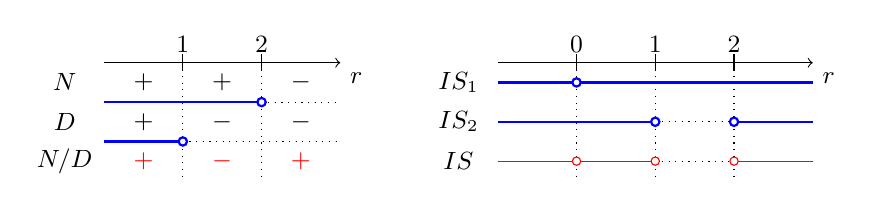
\begin{tikzpicture}[font=\small,x=10mm, y=10mm]

\draw[->] (0,0) -- (3,0) node [below right] () {$r$};
\draw[->] (5,0) -- (9,0) node [below right] () {$r$};

\foreach \x in {1,2,6,7,8}{
\draw(\x,3pt)--(\x,-3pt);
\begin{scope}[dotted]
\draw (\x,0) -- (\x,-1.5);
\draw (2,-.5) -- (3,-.5);
\draw (1,-1) -- (3,-1);
\draw (7,-.75) -- (8,-.75);
\draw (7,-1.25) -- (8,-1.25);
\end{scope}}

\node[above]  at (1,0) {$1$};
\node[above]  at (2,0) {$2$};
\node[above]  at (6,0) {$0$};
\node[above]  at (7,0) {$1$};
\node[above]  at (8,0) {$2$};

\begin{scope}[blue,thick]
\draw (0,-.5) -- (2,-.5);
\draw (1,-1) -- (0,-1);
\draw (5,-.25) -- (6,-.25);
\draw (5,-.25) -- (9,-.25);
\draw (5,-.75) -- (7,-.75);
\draw (8,-.75) -- (9,-.75);

\draw[fill=white] (2,-.5)circle (1.5pt);
\draw[fill=white] (1,-1)circle (1.5pt);
\draw[fill=white] (6,-.25)circle (1.5pt);
\draw[fill=white] (7,-.75)circle (1.5pt);
\draw[fill=white] (8,-.75)circle (1.5pt);
\end{scope}

\foreach \x in {4.5}{
\node  at (\x,-.25) {$IS_1$};
\node  at (\x,-.75) {$IS_2$};
\node  at (\x,-1.25) {$IS$};
}
\foreach \x in {-0.5}{
\node  at (\x,-.25) {$N$};
\node  at (\x,-.75) {$D$};
\node  at (\x,-1.25) {$N/D$};
}

\foreach \z in {.5,1.5}
\node  at (\z,-.25) {$+$};

\foreach \zi in {1.5,2.5}
\node  at (\zi,-.75) {$-$};

\node  at (2.5,-.25) {$-$};
\node  at (0.5,-.75) {$+$};

\begin{scope}[red]
\foreach \y in {-1.25}{
\foreach \ziv in {1.5}
	\node at (\ziv,\y) {$-$};
\foreach \zv in {.5,2.5}
\node at (\zv,\y) {$+$};
\draw (5,-1.25) -- (7,-1.25);
\draw (8,-1.25) -- (9,-1.25);
\draw[fill=white] (6,-1.25)circle (1.5pt);
\draw[fill=white] (7,-1.25)circle (1.5pt);
\draw[fill=white] (8,-1.25)circle (1.5pt);

}
\end{scope}
\end{tikzpicture}

\end{center}
ricaviamo $\IS_{2} = \{k \in \insR | k \ldots \ldots \ldots \vee k > \ldots \ldots \ldots \}$.
Dal grafico a destra inoltre otteniamo $\IS = \IS_{1} \cap \IS_{2} = \{ k \in \insR | k
\ldots \ldots \ldots \vee 0 < k < \ldots \ldots \vee k \ldots \ldots \ldots \}$.
\end{esercizio}

\begin{esercizio}
 \label{ese:3.92}
Assegnata l’equazione $(k + 1) x^{2} + (k + 3) x + k = 0$ stabilire per quale valore di $k$ una sua soluzione è $x =-1$. In tale caso determinare l’altra soluzione.

\emph{Traccia di svolgimento}:
Ricordiamo che un valore numerico è soluzione di un'equazione se sostituito all’incognita trasforma l’equazione in una uguaglianza vera.
Per questo motivo, sostituendo all’incognita il valore assegnato, il parametro $k$ dovrà verificare l’uguaglianza: $(k + 1) (- 1)^{2} + (k + 3) (- 1) + k = 0 \Rightarrow\ldots\ldots\ldots\ldots$
Sostituendo il valore di $k$ trovato, l’equazione diventa: $3 x^{2} + 5 x + 2 = 0$; l’altra soluzione può essere trovata o con la formula risolutiva, oppure
ricordando che $x_{1} + x_{2}=- \frac{b}{a}=- \frac{5}{3}$ da cui $x_{2}=\ldots\ldots$ o anche $x_{1} \cdot x_{2}=\frac{c}{a}=\frac{2}{3}$ da cui $x_{2}=\ldots\ldots$
\end{esercizio}

\begin{esercizio}
 \label{ese:3.93}
Giustificare la verità della seguente proposizione: “per qualunque valore assegnato al parametro $m$ l’equazione $(m-1) x^{2} + 2 m x + m + 1 = 0$
ha soluzioni reali distinte”.
Determinare inoltre $m$ affinché: a) $x_{1} + x_{2} = 1-\sqrt{3}$;\quad b) $ x_{1} \cdot x_{2} = \frac{12}{5}$;\quad c) $x_{1} + x_{2} = 1-x_{1} \cdot x_{2}$.
\end{esercizio}

\begin{esercizio}
 \label{ese:3.94}
Nell’equazione $7 x^{2} + (k-5) x-(k + 2) = 0$ determinare $k$ affinché le soluzioni siano reali; distingui i casi “reali coincidenti” e “reali distinte”.
Nel primo caso determina $x_{1} = x_{2} = \ldots \ldots$; nel secondo caso, determina $k$ affinché
\begin{enumeratea}
\item il prodotto delle soluzioni sia $- \frac{8}{3}$;
\item una soluzione sia nulla;
\item le soluzioni siano una il reciproco dell’altra, cioè: $x_{1} = \frac {1} {x_{2}}$;
\item la somma dei reciproci delle soluzioni sia $\frac{1} {2}$;
\item la somma delle soluzioni superi il loro prodotto di $2$.
\end{enumeratea}
\end{esercizio}

\begin{esercizio}
 \label{ese:3.95}
Verificare che nell’equazione $(2 m-3) x^{2}-(m + 2) x + 3 m-2 = 0$ si hanno due valori del parametro per cui le soluzioni sono reali coincidenti. Determina i due valori.
\end{esercizio}

\begin{esercizio}
 \label{ese:3.96}
Nell’equazione $x^{2}-2 (k + 2) x + (k^{2}-3 k + 2) = 0$ determinare $k$ affinché le soluzioni siano reali, con somma positiva e prodotto negativo.

\emph{Traccia di svolgimento}:
Il problema richiede tre condizioni alle quali deve soddisfare contemporaneamente il parametro, pertanto si formalizza con il sistema
$\left \{ \begin{array}{l} \Delta \geq 0 \\- \frac{b}{a} > 0\\
\frac{c}{a} < 0 \end{array}\right.$.
\end{esercizio}

\begin{esercizio}[\Ast]
 \label{ese:3.97}
Data l'equazione $x^{2}-2 x-k = 0$ determinare $k$ in modo che
\begin{enumeratea}
\item le soluzioni siano reali e distinte \quad $(\Delta>0)$;
\item la somma delle soluzioni sia $10 \quad (x_{1} + x_{2} = 10)$;
\item il prodotto delle soluzioni sia $10 \quad (x_{1} \cdot x_{2} = 10)$;
\item una soluzione sia uguale a $0$ \quad (sostituire $0$ alla $x$);
\item le radici siano opposte \quad $(x_{1} + x_{2} = 0)$;
\item le radici siano reciproche \quad $(x_{1} \cdot x_{2} = 1)$
\item le radici siano coincidenti \quad $(\Delta=0)$;
\item la somma dei quadrati delle radici sia $12 \quad \left(x_{1}^{2} + x_{2}^{2} = (x_{1} + x_{2})^{2}-2x_{1} x_{2} = 12\right)$;
\item la somma dei reciproci delle radici sia $-4 \quad \left(\frac{1}{x_{1}} + \frac{1}{x_{2}} = \frac{x_{1} +x_{2}}{x_{1} x_{2}} =-4 \right)$
\item la somma dei cubi delle radici sia $1$ \protect\\ $\left( x_{1}^{3} + x_{2}^{3} = (x_{1} + x_{2})^{3}-3x_{1}^{2} x_{2}-3x_{1} x_{2}^{2} = (x_{1} + x_{2})^{3}-3x_{1} x_{2} (x_{1} + x_{2}) = 1\right)$;
\item le radici siano entrambe negative $\left(\left\{\begin{array}{l} x_{1} \cdot x_{2} > 0 \\x_{1} + x_{2} < 0 \end{array}\right.\right)$.
\end{enumeratea}
\end{esercizio}

\begin{esercizio}[\Ast]
 \label{ese:3.98}
Data l'equazione $x^{2}-k x-1 = 0$ determinare $k$ in modo che
\begin{enumeratea}
\item le soluzioni siano coincidenti;
\item la somma delle radici sia $8$;
\item le radici siano opposte;
\item una radice sia $- \frac{1}{3}$;
\item il prodotto delle radici sia $-1$.
\end{enumeratea}
\end{esercizio}

\begin{esercizio}[\Ast]
 \label{ese:3.99}
Data l'equazione $x^{2} + (k + 1) x + k = 0$ determinate $k$ affinché l'equazione
\begin{enumeratea}
\item abbia una soluzione sia uguale a zero;
\item abbia soluzioni opposte;
\item non abbia soluzioni reali;
\item abbia le radici reciproche;
\item abbia le radici positive (regola di Cartesio).
\end{enumeratea}
\end{esercizio}

\begin{esercizio}[\Ast]
 \label{ese:3.100}
Data l'equazione $x^{2}-kx + 6 = 0$ determinate $k$ affinché
\begin{enumeratea}
\item abbia la somma delle radici uguale a $7$;
\item abbia le radici reali e opposte;
\item abbia la somma dei reciproci delle radici uguale a $-6$;
\item abbia una radice uguale a $- \frac{3}{2}$;
\end{enumeratea}
\end{esercizio}

\begin{esercizio}[\Ast]
 \label{ese:3.101}
Data l'equazione $x^{2} + (k + 1) x + k^{2} = 0$ determinare $k$ affinché
\begin{enumeratea}
\item abbia come soluzione $-1$;
\item abbia una soluzione doppia $(x_1 =x_2)$;
\item abbia le radici reciproche;
\item abbia una radice l'opposto della reciproca dell'altra $\left(x_1=-\frac{1}{x_2}\rightarrow x_1 \cdot x_2=-1\right)$;
\item abbia una radice nulla.
\end{enumeratea}
\end{esercizio}

\begin{esercizio}[\Ast]
 \label{ese:3.102}
Data l'equazione $kx^{2}-2kx + k-2 = 0$ determinare $k$ affinché
\begin{enumeratea}
\item abbia una radice nulla;
\item abbia la somma dei reciproci delle radici uguale a $1$;
\item abbia la somma dei quadrati delle radici uguale a $4$;
\item abbia la somma delle radici che superi di $5$ il loro prodotto.
\end{enumeratea}
\end{esercizio}

\begin{esercizio}[\Ast]
 \label{ese:3.103}
Data l'equazione $x (x-a) = \frac{a + x}{a + 2}$ determinate $a$ affinché
\begin{enumeratea}
\item una soluzione sia $1$;
\item l'equazione sia di primo grado;
\item una soluzione sia uguale al reciproco dell'altra;
\item la somma delle soluzioni sia il doppio del loro prodotto;
\item la somma dei quadrati delle soluzioni sia $0$;
\item la somma delle radici sia l'opposto del loro prodotto;
\item le soluzioni siano reali e distinte;
\item l'equazione sia spuria;
\item la somma dei cubi delle soluzioni sia nulla;
\item le soluzioni siano reali e discordi;
\item la somma dei reciproci dei cubi sia $1$.
\end{enumeratea}
\end{esercizio}

\begin{esercizio}[\Ast]
 \label{ese:3.104}
Data l'equazione $kx^{2}-(2k + 1) x + k-5 = 0$ determinare il valore di $k$ per il quale
\begin{enumeratea}
\item l'equazione ha soluzioni reali;
\item il prodotto delle radici sia $-2$;
\item la somma delle radici sia $1$;
\item una soluzione sia $-2$;
\item le soluzioni siano opposte;
\item la somma dei reciproci sia $3$;
\item le soluzioni siano reciproche;
\item una soluzione sia l'opposto del reciproco dell'altra;
\item la somma dei quadrati delle soluzioni sia $4$;
\item le radici siano concordi;
\item le radici siano entrambe negative;
\item la somma delle radici uguagli l'opposto del loro prodotto.
\end{enumeratea}
\end{esercizio}

\begin{esercizio}
 \label{ese:3.105}
 Per quale valore di $k \in \insR$ l'equazione $kx^{2}-x + k = 0$ non ammette soluzioni reali?
\[\boxA\; k \leq-\frac{1}{2} \vee k \geq + \frac{1}{2}\quad\boxB\; - \frac{1}{2} < k < \frac{1}{2}\quad\boxC\; k <-\frac{1}{2} \vee k > \frac{1}{2}\quad\boxD\; - \frac{1}{2} \leq k \leq \frac{1}{2}\]
\end{esercizio}

\begin{esercizio}
 \label{ese:3.106}
Per quale valore di $k \in \insR$ l'equazione $x^{2} + (k-2) x + 1 = 0$ ammette due soluzioni reali e distinte?
\[\boxA\quad k > 4\qquad\boxB\quad k = 0 \vee k = 4\qquad\boxC\quad 0 < k < 4\qquad\boxD\quad k < 0 \vee k > 4\]
\end{esercizio}

\begin{esercizio}
 \label{ese:3.107}
Per quale valore di $k$ l'equazione $(k-1) x^{2} + kx + (k + 1) = 0$ ha una soluzione nulla?
\[\boxA\quad k = 1\qquad\boxB\quad k = -1\qquad\boxC\quad k =0\qquad\boxD\quad \text{nesssun valore di }k\]
\end{esercizio}

\begin{esercizio}
 \label{ese:3.108}
Per quale valore di $k$ l'equazione $kx^{2} + \frac{1}{2} x + 1 = 0$ ha due soluzioni identiche?
\[\boxA\quad k = \frac{1}{4}\qquad\boxB\quad k = \frac{1}{16}\qquad\boxC\quad k = 2\qquad\boxD\quad \text{nesssun valore di }k\]
\end{esercizio}

\begin{esercizio}
 \label{ese:3.109}
Per quale valore di $k$ l'equazione $(k + 3) x^{2}-2x + k = 0$ ammette due soluzioni reciproche?
\[\boxA\quad k = 0\qquad\boxB\quad k = -3\qquad\boxC\quad \text{qualsiasi valore di }k\qquad\boxD\quad \text{nesssun valore di }k\]
\end{esercizio}

\begin{esercizio}
 \label{ese:3.110}
Per quale valore di $k$ l'equazione $(k + 1) x^{2}-kx-4 = 0$ ha una soluzione uguale a $2$?
\[\boxA\quad k = 4\qquad\boxB\quad k =-2\qquad\boxC\quad k = 0\qquad\boxD\quad k =-1\]
\end{esercizio}

\begin{esercizio}
 \label{ese:3.111}
Se l'equazione $(k + 1) x^{2}-kx-4 = 0$ ha una soluzione uguale a $2$ quanto vale l'altra soluzione?
\[\boxA\quad x = 0\qquad\boxB\quad x =-2\qquad\boxC\quad x = \frac{1}{2}\qquad\boxD\quad x = 2\]
\end{esercizio}

\begin{multicols}{2}
%===================================
\subsection*{3.9 - Problemi di secondo grado}

\begin{esercizio}[\Ast]
 \label{ese:3.112}
Il quadrato di un numero reale supera la metà del numero stesso di $ 5 $.
Determina i numeri reali che rendono vera la proposizione enunciata.
\end{esercizio}

\begin{esercizio}[\Ast]
 \label{ese:3.113}
Il prodotto della metà di un numero relativo con il suo successivo è $ 666 $.
Quali numeri verificano questa proprietà?
\end{esercizio}

\begin{esercizio}
 \label{ese:3.114}
Trova un numero positivo che addizionato al proprio quadrato dia come somma $ 156 $.
\end{esercizio}

\begin{esercizio}
 \label{ese:3.115}
Un numero addizionato al quadrato della sua metà, dà come risultato $ 120 $.
Trova il numero.
\end{esercizio}

\begin{esercizio}
 \label{ese:3.116}
Verifica che non esiste alcun numero reale tale che il quadrato del suo
doppio uguagli la differenza tra il triplo del suo quadrato e il quadrato
della somma del numero con $ 3 $.
\end{esercizio}

\begin{esercizio}[\Ast]
 \label{ese:3.117}
Due numeri naturali hanno rapporto $ 2/3 $ e somma dei loro quadrati $ 3757 $.
Individua i numeri che verificano questa proprietà.
\end{esercizio}

\begin{esercizio}[\Ast]
 \label{ese:3.118}
La somma dei quadrati di due numeri pari consecutivi è $ 580 $. Quali sono i
due numeri?
\end{esercizio}

\begin{esercizio}[\Ast]
 \label{ese:3.119}
Di due numeri naturali consecutivi si sa che la somma dei loro reciproci
è $ 9/20 $. Quali sono i due numeri?
\end{esercizio}

\begin{esercizio}[\Ast]
 \label{ese:3.120}
Di cinque numeri interi consecutivi si sa che la differenza tra il quadrato
della somma degli ultimi due numeri e la somma dei quadrati dei primi tre è
$ 702 $. Qual è il più piccolo di questi numeri?
\end{esercizio}

 \begin{esercizio}[\Ast]
 \label{ese:3.121}
La somma delle età di un padre con quella del figlio è $ 34 $. Sapendo che
l'età del padre aumentata di $ 8 $ anni dà il quadrato dell'età del figlio,
trovare le due età.
\end{esercizio}

\begin{esercizio}[\Ast]
 \label{ese:3.122}
Determina due numeri naturali sapendo che la somma tra il doppio del minore
ed il triplo del maggiore è $ 42 $ e che il rapporto tra la loro somma e il loro
prodotto è $ 5/12 $.
\end{esercizio}

\begin{esercizio}[\Ast]
 \label{ese:3.123}
Trova l'età di una persona sapendo che fra tre anni la sua età sarà
uguale al quadrato della quinta parte dell'età che aveva tre anni fa.
\end{esercizio}

\begin{esercizio}[\Ast]
 \label{ese:3.124}
Trova due numeri pari consecutivi tali che la somma del quadrato del minore
con il loro prodotto sia $ 544 $.
\end{esercizio}

\begin{esercizio}[\Ast]
 \label{ese:3.125}
Trova due numeri naturali sapendo che il minore supera di $ 2 $ la terza parte
del maggiore e che il quadrato del maggiore supera di $ 68 $ il quadrato del
doppio del minore.
\end{esercizio}

\begin{esercizio}[\Ast]
 \label{ese:3.126}
Da un segmento di $ 25\unit{cm} $ ne vogliamo ottenere due in modo che la somma dei
loro quadrati sia $ 337 $.
\end{esercizio}

\begin{esercizio}[\Ast]
 \label{ese:3.127}
In una frazione il numeratore e il denominatore hanno somma $ 14 $, mentre la
somma dei loro quadrati è $ 106 $. Qual è la frazione?
\end{esercizio}

\begin{esercizio}[\Ast]
 \label{ese:3.128}
Due navi partono contemporaneamente da uno stesso porto e arrivano alla
stessa destinazione dopo aver percorso sulla stessa rotta a velocità
costante $ 720\unit{miglia} $. Sapendo che una delle due navi viaggia con una velocità
di 1 nodo (1 miglio all'ora) superiore a quella dell'altra nave e che perciò
arriva 3 ore prima a destinazione, determina le velocità in nodi delle due
navi.
\end{esercizio}

\begin{esercizio}
 \label{ese:3.129}
Due navi che viaggiano su rotte perpendicolari a velocità costante si
incontrano in mare aperto. Sapendo che una delle navi viaggia a 15 nodi (1
nodo = 1 miglio all'ora), dopo quanto tempo le due navi si trovano alla
distanza di 40 miglia?
\end{esercizio}

\begin{esercizio}
 \label{ese:3.130}
Luca e Carlo bevono due aranciate in bottiglia. Nel tempo in cui Luca beve
11 sorsi, Carlo ne beve 8, ma due sorsi di Carlo equivalgono a tre di Luca.
Quando Carlo inizia a bere Luca ha già preso 4 sorsi. Dopo quanti sorsi di
Carlo le due bibite hanno lo stesso livello?
\end{esercizio}

\begin{esercizio}
 \label{ese:3.131}
Un maratoneta durante un allenamento fa due giri di un percorso di $ 22\unit{km} $
mantenendo in ciascun giro una velocità costante ma nel secondo giro la
velocità è inferiore di $ 0,5\unit{km/h} $ rispetto al primo giro. A quali velocità
ha corso se ha impiegato complessivamente 2 ore e un quarto?
\end{esercizio}

\begin{esercizio}[\Ast]
 \label{ese:3.132}
Un capitale di 12000 euro è depositato in banca a un certo tasso di interesse
annuale. Alla scadenza del primo anno gli interessi maturati vengono
ridepositati sullo stesso conto. Alla scadenza del secondo anno si ritira la
somma di 12854,70 euro. Qual è stato il tasso di interesse?
\end{esercizio}

\begin{esercizio}
 \label{ese:3.133}
In un rettangolo, se si aumenta di 2 metri la base e si riduce di un metro
l’altezza, la sua area aumenta di 4 metri quadrati. Se invece si riduce di
un metro la base e si aumenta di 2 metri l’altezza, l’area aumenta di 22
metri quadrati. Quali sono le dimensioni del rettangolo?
\end{esercizio}

\begin{esercizio}[\Ast]
 \label{ese:3.134}
Una ditta spende mensilmente 73500 in stipendi per i propri dipendenti.
Aumentando di 5 il numero dei dipendenti, ma riducendo l'orario di lavoro,
diminuisce a ciascuno lo stipendio di 200 e spende solamente 2500 in più per
gli stipendi. Quanti dipendenti aveva inizialmente la ditta e quanto
guadagnava ognuno di essi?
\end{esercizio}

\begin{esercizio}[\Ast]
 \label{ese:3.135}
Da un cartoncino rettangolare ($ ABCD $, come in figura) si vuole ritagliare un
quadrato ($ DEFG $) in modo che le due parti ottenute siano equivalenti.
Determinare la misura del lato del quadrato sapendo che
$\overline {EC} = 6\unit{cm} $ e $\overline {AG} = 4\unit{cm}$.
\begin{center}
 % (c) 2013 Claudio Carboncini - claudio.carboncini@gmail.com
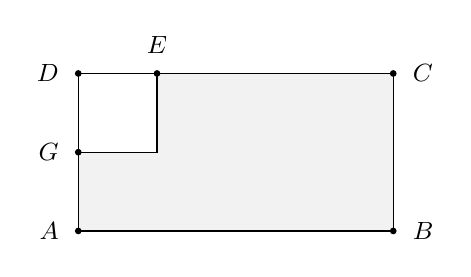
\begin{tikzpicture}[x=10mm,y=10mm,font=\small]

  \fill[fill=gray!10] (1,1) rectangle (5,3);
  \fill[fill=white] (1,3) rectangle (2,2);
  \draw (1,1) rectangle (5,3);
  \draw (1,3) rectangle (2,2);
  \node [label={[name=label node]left:$A$}] at (1,1) {};
  \node [label={[name=label node]left:$D$}] at (1,3) {};
  \node [label={[name=label node]right:$C$}] at (5,3) {};
  \node [label={[name=label node]right:$B$}] at (5,1) {};
  \node [label={[name=label node]left:$G$}] at (1,2) {};
  \node [label={[name=label node]above:$E$}] at (2,3) {};

  \foreach \x in {1,5}
    \foreach \y in {1,3}
      \filldraw[fill=black, draw=black]  (\x,\y) circle (1pt);
      \filldraw[fill=black, draw=black]  (1,2) circle (1pt);
      \filldraw[fill=black, draw=black]  (2,3) circle (1pt);

\end{tikzpicture}

\end{center}
\end{esercizio}

\begin{esercizio}[\Ast]
 \label{ese:3.136}
Un terreno a forma rettangolare di $6016\unit{m^2}$ viene recintato con un muro lungo
$350\unit{m}$. Quali sono le dimensioni del rettangolo?
\end{esercizio}

\begin{esercizio}[\Ast]
 \label{ese:3.137}
Determinare sul segmento $ AB $ di misura $ 5\unit{m} $ un punto $ P $ tale che il rettangolo
delle due parti sia equivalente al quadrato di lato $ 2\unit{m} $. Rappresenta con un
disegno le soluzioni.
\end{esercizio}

\begin{esercizio}[\Ast]
 \label{ese:3.138}
Calcolare perimetro e area del triangolo $ ABC $ isoscele sulla base $ AB $ sapendo
che la differenza tra la base e l’altezza ad essa relativa è $ 0,5\unit{m} $ e tale
è anche la differenza tra il lato $ CB $ e la base stessa.
\end{esercizio}

\begin{esercizio}[\Ast]
 \label{ese:3.139}
La superficie del rettangolo $ ABCD $ supera di $ 119\unit{m^2} $ la superficie del quadrato
costruito sul lato minore $ AD $. Determinare il perimetro e la misura della
diagonale sapendo che i $ 7/10 $ del lato maggiore AB sono uguali ai $ 12/5 $ del
lato minore.
\end{esercizio}

\begin{esercizio}[\Ast]
 \label{ese:3.140}
Nel trapezio rettangolo $ ABCD $, il rapporto tra la base maggiore $ AB $ e la base
minore $ CD $ è $ 8/5 $, il lato obliquo forma con $ AB $ un angolo di $ 45\grado $. Determinare
il perimetro sapendo che l’area è $312\unit{m^2}$.
\end{esercizio}

\begin{esercizio}[\Ast]
 \label{ese:3.141}
Determina il perimetro di un rombo che ha l'area di $24\unit{m^2}$ e il rapporto tra
le diagonali $ 4/3 $.
\end{esercizio}

\begin{esercizio}[\Ast]
 \label{ese:3.142}
Un rettangolo $ ABCD $ ha il perimetro di $ 48\unit{cm} $ e l'area di $ 128\unit{cm^2} $. A una certa
distanza $x$ dal vertice $ A $ sui due lati $ AD $ e $ AB $ si prendono rispettivamente i
punti $ P $ e $ Q $. Alla stessa distanza $ x $ dal vertice $ C $ sui lati $ CB $ e $ CD $ si
prendono rispettivamente i punti $ R $ e $ S $. Sapendo che il rapporto tra l'area
del rettangolo $ ABCD $ e l'area del quadrilatero $ PQRS $ è $ 32/23 $ calcola la
distanza $x$.
\end{esercizio}

\begin{esercizio}
 \label{ese:3.143}
Un trapezio rettangolo ha la base minore di $ 9|unit{cm} $, l'altezza i $ 2/9 $ della base
maggiore e l'area di $20 + 9 \sqrt{2}\unit{cm^{2}}$. Determina la misura della base maggiore.
\end{esercizio}

\begin{esercizio}[\Ast]
 \label{ese:3.144}
Da un quadrato di $ 32\unit{cm} $ di lato vengono ritagliati due triangoli rettangoli
come descritti in figura. Calcola la misura di $ x $,
inferiore alla metà del lato del quadrato, in modo che l’area totale dei
due triangoli evidenziati sia pari a $ 344\unit{cm^2} $.
\begin{center}
 % (c) 2013 Claudio Carboncini - claudio.carboncini@gmail.com
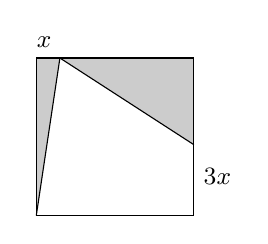
\begin{tikzpicture}[x=10mm,y=10mm,font=\small]

  \fill[fill=gray!40] (1,1) -- (1,3) -- (1.3,3);
  \fill[fill=gray!40] (1.3,3) -- (3,3) -- (3,1.9);
  \draw (1,1) rectangle (3,3);
  \draw (1.3,3)--(1,1);
  \draw (3,1.9)--(1.3,3);
  \node (x) at (1.1,3.2) {$x$};
  \node (h) at (3.3,1.5) {$3x$};

\end{tikzpicture}

\end{center}
\end{esercizio}

\begin{esercizio}[\Ast]
 \label{ese:3.145}
Il rettangolo $ ABCD $ ha l’area di $ 558\unit{cm^2} $ e il lato $ DC $ di $ 18\unit{cm} $. Lo si
vuole trasformare in un nuovo rettangolo $ AEFG $ accorciando l’altezza di una quantità $ 5x $ e allungando la base di
una quantità $ 4x $ in modo che il nuovo rettangolo $ AEFG $ che abbia l’area di
$ 228\unit{cm^2} $. Determina la quantità $ x $ necessaria a compiere la trasformazione
richiesta.
\end{esercizio}

\begin{esercizio}[\Ast]
 \label{ese:3.146}
Il rettangolo $ AEFG $ ha l’area di $ 768\{cm^2\} $ e l’altezza $ AG $ di $ 24\unit{cm} $. Si
vuole allungare l’altezza di una quantità
$ x $ e accorciare la base di una quantità doppia $ 2x $ in modo da ottenere un
secondo rettangolo $ ABCD $ che abbia l’area di $ 702\unit{cm^2} $. Determina $ x $.
\end{esercizio}

\begin{esercizio}
 \label{ese:3.147}
Un trapezio isoscele di area $ 144\unit{cm^2} $ ha la base maggiore che supera di $ 10\unit{cm} $
la base minore che a sua volta supera di $ 10\unit{cm} $ l'altezza. Determina il perimetro del trapezio.
\end{esercizio}

\begin{esercizio}[\Ast]
 \label{ese:3.148}
Il rettangolo $ ABCD $ ha l’area di $ 240\unit{cm^2} $ e l’altezza $ AD $ di $ 12\unit{cm} $. Si
vuole trasformare il rettangolo in un triangolo $ AEF $ allungando l’altezza di una quantità $ 3x $ e accorciando la
base di una quantità $ x $ (vedi figura) in modo che il nuovo triangolo $ AEF $ abbia l’area di $ 162\unit{cm^2} $.
\begin{center}
 % (c) 2013 Claudio Carboncini - claudio.carboncini@gmail.com
\begin{tikzpicture}[x=10mm,y=10mm,font=\small]
  \draw (1,1) rectangle (5,2); %ABCD
  \draw (1,1)--(2.6,4.4); %AF
  \draw (4.2,1)--(2.6,4.4); %EF
  \draw [dashed] (2.6,4.4) -- (2.6,2);
  \draw [dotted] (2.6,2) -- (2.6,1);
  \node (x) at (4.6,.7) {$x$};
  \node (h) at (2.3,3) {$3x$};
  \node [label={[name=label node]below left:$A$}] at (1,1) {};
  \node [label={[name=label node]above left:$D$}] at (1,2) {};
  \node [label={[name=label node]above right:$C$}] at (5,2) {};
  \node [label={[name=label node]below right:$B$}] at (5,1) {};
  \node [label={[name=label node]below:$E$}] at (4.2,1) {};
  \node [label={[name=label node]above:$F$}] at (2.6,4.4) {};

%  \foreach \x in {1,5}
%    \foreach \y in {1,2}
%      \filldraw[fill=black, draw=black]  (\x,\y) circle (1pt);
%      \filldraw[fill=black, draw=black]  (2.6,4.4) circle (1pt);
%      \filldraw[fill=black, draw=black]  (4.2,1) circle (1pt);

\end{tikzpicture}

\end{center}
\end{esercizio}

\begin{esercizio}[\Ast]
 \label{ese:3.149}
La piramide di Cheope è a base quadrata ed ha una superficie totale pari a
$ 135700\unit{m^2} $. Sapendo che l’apotema della piramide misura $ 180 $ metri, si
calcoli la lunghezza del lato di base.
\end{esercizio}

\begin{esercizio}[\Ast]
 \label{ese:3.150}
Un container a forma di parallelepipedo a base quadrata ha una superficie
totale pari a $ 210\unit{m^2} $. L’altezza è il doppio del lato di base diminuito di
$ 2 $ metri. Trovare la lunghezza del lato di base.
\end{esercizio}

\subsection*{3.10 - Problemi con un parametro}

\begin{esercizio}
 \label{ese:3.151}
Sul prolungamento dei lati $ AB $, $ BC $, $ CD $, $ DA $ del quadrato $ ABCD $ prendi rispettivamente i punti $ Q $, $ R $, $ S $, $ P $ in modo che $ QB=RC=SD=PA $. Dimostra che $ PQRS $ è un quadrato; nell’ipotesi che sia $AB = 3\unit{m}$ determina $\overline {AP}$ in modo che l’area di $ PQRS $ sia $ k $, con $ k $ reale positivo.
\begin{center}
 % (c) 2013 Claudio Carboncini - claudio.carboncini@gmail.com
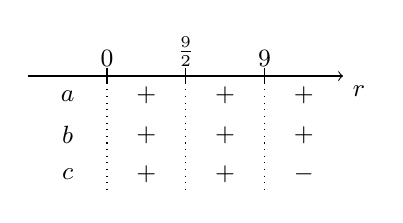
\begin{tikzpicture}[font=\small,x=10mm, y=10mm]

\draw[->] (0,0) -- (4,0) node [below right] () {$r$};

\foreach \x in {1,2,3}{
\draw(\x,3pt)--(\x,-3pt);
\begin{scope}[dotted]
\draw (\x,0) -- (\x,-1.5);
\end{scope}}

\node[above]  at (1,0) {$0$};
\node[above]  at (2,0) {$\frac 9 2$};
\node[above]  at (3,0) {$9$};

\foreach \x in {0.5}{
\node  at (\x,-.25) {$a$};
\node  at (\x,-.75) {$b$};
\node  at (\x,-1.25) {$c$};
}

\foreach \z in {1.5,2.5,3.5}
\node  at (\z,-.25) {$+$};

\foreach \zi in {1.5,2.5,3.5}
\node  at (\zi,-.75) {$+$};

\node  at (1.5,-1.25) {$+$};
\node  at (2.5,-1.25) {$+$};
\node  at (3.5,-1.25) {$-$};
\end{tikzpicture}

\end{center}
\emph{Svolgimento}:
per dimostrare che $ PQRS $ è un quadrato dobbiamo dimostrare che i lati sono
congruenti e che gli angoli sono retti. Se si pone $\overline{AP} = x$ con $x > 0$.
$\Area(PQRS)= \overline {PQ}^{2} = \overline {PA}^{2} + \overline{AQ}^{2}$per il teorema di Pitagora.
Verifica che si ottiene l’equazione risolvente $2 x^{2} + 6 x + (9-k) = 0$. Poiché vogliamo soluzioni reali positive, discuti l’equazione con il metodo di Cartesio. Il discriminante è $\Delta = 36-8 (9-k)$ pertanto l'equazione ammette soluzioni reali per $k \geq \frac{9}{2}$. Dal segno dei coefficienti, essendo i primi due coefficienti positivi si ha una permanenza e quindi una radice negativa che non è accettabile. Per ottenere una soluzione positiva ci deve essere una variazione di segno negli ultimi due coefficienti, in altre parole $9-k$ deve essere negativo cioè $9-k < 0 \rightarrow k > 9$. Pertanto il problema ha soluzioni per $k > 9$.
\end{esercizio}

\begin{esercizio}
 \label{ese:3.152}
Nel trapezio rettangolo $ ABCD $ di base maggiore $ BC $, la diagonale $ AC $ è bisettrice dell’angolo $B \widehat {C} D$. Posto $\overline {AB} = 1\unit{m}$, determina la base maggiore in modo che sia $ 2k $ il perimetro del trapezio. Imposta dati e obiettivo del problema.
\begin{center}
 % (c) 2013 Claudio Carboncini - claudio.carboncini@gmail.com
\begin{tikzpicture}[x=10mm,y=10mm,font=\small]

  \coordinate(a) at (0,2.598);%il punto A
  \coordinate(b) at (0,0);%il punto B
  \coordinate(c) at (4.5,0);%il punto C
  \coordinate(d) at (3,2.598);%il punto D
  \coordinate (h) at ($(a)!(d)!(c)$);%trova le coordinate della proiezione di D su a--c
  \coordinate (h1) at ($(a)!{1/2}!(h)$);
  \coordinate (h2) at ($(h)!{1/2}!(c)$);
  \coordinate (a1) at ($(a)!{1/2}!(d)$);
  \coordinate (d1) at ($(d)!{1/2}!(c)$);
  \draw (a) -- (b)  -- (c) -- (d) -- cycle;%disegna il trapezio
  \draw [] (d) -- (h);%perpendicolare da D a a--c
  \draw [] (a) -- (c);%la diagonale del trapezio
  \draw (h1) node {$//$} ;
  \draw (h2) node {$//$} ;
  \draw (a1) node {$\times$} ;
  \draw (d1) node {$\times$} ;
  \draw (4.1,0.4) node {$\bullet$} ;
  \draw (3.95,0.12) node {$\bullet$} ;
  \node [label={[name=label node]above:$A$}] at (a) {};
  \node [label={[name=label node]below:$B$}] at (b) {};
  \node [label={[name=label node]below:$C$}] at (c) {};
  \node [label={[name=label node]above:$D$}] at (d) {};
  \node [label={[name=label node]below:$H$}] at (h) {};

\end{tikzpicture}

\end{center}
\emph{Svolgimento}: poniamo $\overline {BC} = x$. Dall’informazione che la diagonale $ AC $ è bisettrice dell’angolo $B \widehat {C} D$, possiamo dimostrare che $ ADC $ è un triangolo isoscele sulla base $ AC $. L’equazione risolvente sarà determinata dalla relazione tra i lati che esprime il perimetro del trapezio. Dobbiamo quindi esprimere $\overline {DC}$ in funzione di $ x $. Traccia l’altezza $ DH $ del triangolo isoscele $ ADC $ e dopo aver dimostrato la similitudine di $ ABC $ con $ DHC $, osserva che si ha $DC : AC = HC : BC$ poiché $HC = \frac{1}{2} AC$ si ha $\frac{1}{2} \overline {AC}^{2} = \overline {DC} \cdot \overline {BC}$ da cui si può ricavare la misura di $ DC = \frac{1}{2} \frac{AC^{2}}{BC}$. Dato che $\overline {AC}^{2}=1+x^2$, per il teorema di Pitagora applicato al triangolo $ ABC $, quindi $ DC = \frac{1 + x^2} {2 x} $ L’equazione parametrica risolvente è $2 x^{2} + x \cdot (1-2 k) + 1 = 0$ con $x > 0$ che può essere discussa con il metodo di Cartesio.
\end{esercizio}

\begin{esercizio}
 \label{ese:3.153}
Il quadrilatero $ ABCD $ ha le diagonali perpendicolari ed è inscritto in una circonferenza; sapendo che $\overline{AB} = 5a$; $\overline {AE} = 3 a$; $2 p_{BCA} = \frac{5}{2} \cdot \overline {BD}$, essendo $ E $ punto d’incontro delle diagonali, determinate la misura delle diagonali. Poni $\overline {CE} = x$.
\end{esercizio}

\begin{esercizio}
 \label{ese:3.154}
Il rettangolo $ ABCD $ ha i lati $ AB $ e $ BC $ che misurano rispettivamente $ a $ e $ 3a $ (con $ a\geq 0 $). Prolunga il lato $ AB $ di due segmenti congruenti $ BN $ e $ AM $ e sia $ V $ il punto di intersezione delle retta $ MD $ e $ CN $. Posto $\overline {BN} = x$, determina la misura della base $ MN $ del triangolo $ MVN $ in modo che la sua area sia $ k $ volte l’area del rettangolo assegnato.
\end{esercizio}

\begin{esercizio}
 \label{ese:3.155}
Due numeri reali hanno come somma $ a $ con $(a \in \insR_{0})$; determinare i due numeri in modo che il loro prodotto sia $ k $ con $(k \in \insR_{0})$. Quale condizione si deve porre sull’incognita? Per quale valore del parametro i due numeri soluzione sono uguali?
\end{esercizio}

\begin{esercizio}
 \label{ese:3.156}
In un triangolo rettangolo l’altezza $ AH $ relativa all’ipotenusa $ BC $ misura $ 1\unit{m} $ e $A \widehat {B} C = 60\grado$. Determinare sulla semiretta $ AH $, esternamente al triangolo, un punto $ P $ in modo che sia $ k $ la somma dei quadrati delle distanze di $ P $ dai vertici del triangolo. Quale condizione va imposta al parametro $ k $ perché il problema abbia significato?
\end{esercizio}

\begin{esercizio}
 \label{ese:3.157}
$\overline {AB} = 16 a$; $\overline {BC} = 2 a \sqrt{14}$ rappresentano le misure dei lati del rettangolo $ ABCD $; determinare un punto $ P $ del segmento $ AB $ tale che la somma dei quadrati delle sue distanze dai vertici $ C $ e $ D $ sia uguale al quadrato della diagonale $ DB $. Posto $\overline {AP} = x$ quale delle seguenti condizioni deve rispettare la soluzione? Dopo aver risolto il problema spiegare il significato delle soluzioni ottenute.
\end{esercizio}

\begin{esercizio}
 \label{ese:3.158}
Ad una sfera di raggio $ 1\unit{m} $ è circoscritto un cono il cui volume è $ k $ volte il volume della sfera. Determina l’altezza del cono.
\begin{center}
 % (c) 2013 Claudio Carboncini - claudio.carboncini@gmail.com
\begin{tikzpicture}[x=10mm,y=10mm,font=\small,scale=1.3]

  \coordinate(a) at (0,0);%il punto A
  \coordinate(v1) at (70:5);%il punto V1
  \coordinate(o) at (35:1.5);%il centro del cerchio O
  \coordinate(h) at (1.23,0);%il punto H
  \coordinate (b) at (2.46,0);%il punto B
  \coordinate(v2) at (1.23,6);%il punto v2
  \coordinate (v) at (intersection of a--v1 and h--v2);
  \coordinate (c) at ($(v)!(o)!(b)$);%trova le coordinate della proiezione di o su v--b
  \draw[] (o) circle (0.86);%disegna il cerchio di centro
  \draw[] (v) -- (a) -- (b) -- cycle;%disegna v2--h--a
  \draw[dashed] (v) -- (h);%disegna v--h
  \draw[dashed] (o) -- (c);%disegna o--c
  \draw (h) ellipse (1.23cm and 0.4cm);
  \node [label={[name=label node]above:$V$}] at (v) {};
  \node [label={[name=label node]left:$A$}] at (a) {};
  \node [label={[name=label node]below:$H$}] at (h) {};
  \node [label={[name=label node]right:$B$}] at (b) {};
  \node [label={[name=label node]left:$O$}] at (o) {};
  \node [label={[name=label node]right:$C$}] at (c) {};
\begin{comment}
  \coordinate (h2) at ($(h)!{1/2}!(c)$);
  \coordinate (a1) at ($(a)!{1/2}!(d)$);
  \coordinate (d1) at ($(d)!{1/2}!(c)$);
  \draw (a) -- (b)  -- (c) -- (d) -- cycle;%disegna il trapezio
  \draw [] (d) -- (h);%perpendicolare da D a a--c
  \draw [] (a) -- (c);%la diagonale del trapezio
  \draw (h1) node {$//$} ;
  \draw (h2) node {$//$} ;
  \draw (a1) node {$\times$} ;
  \draw (d1) node {$\times$} ;
  \draw (4.1,0.4) node {$\bullet$} ;
  \draw (3.95,0.12) node {$\bullet$} ;
\end{comment}
\end{tikzpicture}

\end{center}

\emph{Dati}: $ \overline {OC} = 1 $, $ \overline {OC} = \overline {OH} $, $ OC \perp VB $,\protect\\ $ \overline {BC} = \overline {BH} $, $ \overline {AH} = \overline {HB} $, $ VH \perp AB $,\protect\\ $ \text{Volume(cono)} = k \cdot \text{Volume(sfera)} $.

\emph{Obiettivo}: $\overline {VH}$

\emph{Svolgimento}: Poniamo $\overline {VO} = x$ con $x > 0$ da cui $\overline {VH}= \overline {VO} + \overline {OH} = x + 1$.

Ricordiamo che $V\text{(cono)} = \frac{1}{3} \pi \overline {HB}^{2} \cdot \overline {VH}$ e $V\text{(sfera)} = \frac{4}{3} \pi \overline {CO}^{3}$. Per impostare l’equazione risolvente dobbiamo cercare di esprimere $\overline {HB}^{2}$ in funzione di $ x $. Verifica che dalla similitudine di $ VOC $ con $ VHB $ si deduce: $\overline {HB} : \overline {OC} = \overline {VH} : \overline{VC}$ quindi $\overline {HB} = \frac{\overline {OC} \cdot \overline
{VH}}{\overline {VC}}$; dobbiamo ancora ricavare $\overline {VC}$ che per il teorema di Pitagora su $ VCO $ è \ldots Sostituendo tutti gli elementi trovati nella relazione che lega il volume del cono con il volume della sfera, verifica che si ottiene $x^{2} + 2 x (1-2 k) + 4 k = 0$ con $x > 0$, da discutere con il metodo di Cartesio.
\end{esercizio}

\end{multicols}
\begin{esercizio}[\Ast]
 \label{ese:3.159}
 Scheda di ripasso sulle equazioni
\begin{enumerate}
	\item L'equazione $25x^{2} + 1 = 0$ ha per soluzioni:

\boxA\quad $ x = \pm 5 $\qquad \boxB\quad $x = \pm \frac{1}{5}$\qquad\boxC\quad $x = 4 \vee x = 1$\qquad\boxD\quad non ha soluzioni reali

	\item L'equazione $16x^{2} + x = 0$ ha per soluzioni:

\boxA\quad $ x = 4 \vee x = 1 $\quad \boxB\quad $x = \pm \frac{1}{4}$\quad\boxC\quad $x =-\frac{1}{16} \vee x = 0$\quad\boxD\quad non ha soluzioni reali

	\item L'equazione $4x^{2}-9x = 0$ ha per soluzioni:

\boxA\quad $ x = \pm \frac{3}{2} $\qquad \boxB\quad $x = \pm \frac{9}{4}$\qquad\boxC\quad $x = \frac{3}{2} \vee x = 0$\qquad\boxD\quad $x = \frac{9}{4} \vee x = 0$

	\item L'equazione $9x^{2} + 6x + 1 = 0$ ha per soluzioni:

\boxA\quad $x = \pm 3$\qquad\boxB\quad $x = \pm \frac{1}{3}$\qquad\boxC\quad $x =-\frac{1}{3}$ doppia\qquad\boxD\quad non ha soluzioni reali

	\item L'equazione $x^{2}-6x + 36 = 0$ ha per soluzioni:

\boxA\quad $x = \pm 6$\qquad\boxB\quad $x = \pm \sqrt{6}$\qquad\boxC\quad $x =6$ doppia\qquad\boxD\quad non ha soluzioni reali

	\item Quale di queste equazioni ammette una soluzione doppia $ x=3 $?

\boxA\quad $2x^{2}-12x + 18 = 0$\quad\boxB\quad $9-x^{2} = 0$\quad\boxC\quad $x^{2} + 6x + 9 = 0$\quad\boxD\quad $ 3x^{2} + 9x = 0 $

	\item Quale equazione di secondo grado si ottiene con soluzioni $ x_1=1 $ e $ x_2=3 $?

\boxA\quad $x^{2} + x-1 = 0$\quad\boxB\quad $x^{2}-4x + 3 = 0$\quad\boxC\quad $x^{2}-4x-3 = 0$\quad\boxD\quad $ x^{2} + 4x-3 = 0 $

	\item Il polinomio$x^{2} + 5x + 6$ può essere scomposto in:

\boxA\; $(x + 2) (x-3)$\quad\boxB\; $(x + 5) (x + 1)$\quad\boxC\; $(x-2) (x-3)$\quad\boxD\; nessuna delle risposte precedenti

	\item Una delle soluzioni dell'equazione $x^{2}-(\sqrt{2} + 1) x + \sqrt{2} = 0$ è $\sqrt{2}$, quanto vale l'altra?

\boxA\quad $ - \sqrt{2} $\qquad \boxB\quad $\frac{1}{\sqrt{2}}$\qquad\boxC\quad $\sqrt{2} + 1$\qquad\boxD\quad $1$

	\item Per quale valore di $ k $ l'equazione $(2k-1) x^{2} + (2k + 1) x + k-2 = 0$ diventa di I° grado?

\boxA\quad $k = \frac{1}{2}$\qquad \boxB\quad $k =-\frac{1}{2}$\qquad\boxC\quad $k = 2$\qquad\boxD\quad $k = 0$

	\item L'equazione $4m^{2} x^{2}-5mx + 1 = 0$ con parametro $ m $ ha per soluzioni:

\boxA\; $x = m \vee x = 4m$\quad \boxB\; $x = \frac{1}{m} \vee x = \frac{1}{4m}$\quad\boxC\; $x = 64m \vee x = 1$\quad\boxD\; $x = m \vee x = \frac{1}{4}$

	\item L’equazione di secondo grado $x^{2} + (a + 1) x + a = 0$ con $ a $ parametro reale ha come soluzioni:

\boxA\; $x = 1 \vee x = a$\quad \boxB\; $x = a-1 \vee x = 1$\quad\boxC\; $x =-a \vee x =-1$\quad\boxD\; $x = a + 1 \vee x = a$

	\item L’equazione $x^{2} + (t-2) = 0$ con $ t $ parametro reale ammette soluzioni reali per:

\boxA\quad $t \leq 2$\qquad \boxB\quad $t \geq 2$\qquad\boxC\quad $t < 2$\qquad\boxD\quad nessuna delle risposte precedenti

	\item Quanto vale il prodotto delle soluzioni dell'equazione $x^{2}-6a^{2} x + 8a^{4} = 0$?

\boxA\quad $8a^{4}$\qquad \boxB\quad $8a^{2}$\qquad\boxC\quad $6a^{2}$\qquad\boxD\quad non esiste

	\item Il polinomio $x^{2} + (m-2) x-2m$ con $ m $ parametro reale può essere scomposto in:

\boxA\; $(x + m) (x + 1)$\quad\boxB\; $(x + m) (x-2)$\quad\boxC\; $(x + m) (x + 2)$\quad\boxD\; $(x-m) (x-2)$

	\item L’equazione $x^{2} + (k-1) x = 0$ con $ k $ parametro reale:

\boxA\; non ha soluzioni reali\quad\boxB\; ha una soluzione uguale a zero

\boxC\; due soluzioni reali coincidenti per $ k=0 $\quad\boxD\;soluzioni reali e distinte per $ k=1 $

	\item L’equazione $x^{2} + 2x + k-2 = 0$ con $ k $ parametro reale:

\boxA\quad ha due soluzioni reali coincidenti per $ k=3 $

\boxB\quad ha due soluzioni reali coincidenti per $ k=1 $

\boxC\quad ha una soluzione nulla per $k =-2$

\boxD\quad ha soluzioni reali e distinte per $k \neq 3$

	\item L’equazione $x^{2} + m^{2} + 1 = 0$ con $m$ parametro reale:

\boxA\; ammette due soluzioni reali e opposte\quad\boxB\; ammette due soluzioni coincidenti

\boxC\; non ammette soluzioni reali\quad\boxD\; ammette due soluzioni negative

	\item L’equazione $2x^{2} + k^{2} = 0$ con $k$ parametro reale ammette:

\boxA\; due soluzioni reali e distinte\quad\boxB\; due soluzioni reali solo se $k>0$

\boxC\; soluzioni coincidenti per $k = 0$\quad\boxD\; nessuna delle risposte precedenti è corretta

	\item L’equazione $tx^{2}-1 = 0$

\boxA\; ha come soluzioni $x_{1} = 0 \vee x_{2} = 1-t$\quad\boxB\; ammette sempre soluzioni reali

\boxC\; ammette soluzioni reali per $t > 0$\quad\boxD\; ha come soluzioni $x = \pm t$

\end{enumerate}
\end{esercizio}

\subsection{Risposte}
%\begin{multicols}{2}
\paragraph{3.1.} c)~$x_{1}=+4 \vee x_{2}=-4$,\quad f)$\emptyset$,\quad i)~$x_{1} = \sqrt{3} \vee x _{2} = - \sqrt{3}$,\quad l)~$\emptyset$.

\paragraph{3.2.} c)~$x_{1,2} = \frac{\pm \sqrt{15}}{5}$,\quad f)~$x_{1,2} = 0$,\quad i)~$x_{1,2} = \pm 7$,\quad l)~$x_{1,2} = \pm 2$.

\paragraph{3.3.} c)~$x_{1,2} = \pm 5$,\quad f)~$x_{1,2} = \pm \frac{1}{3}$,\quad i)~$x_{1,2} = \pm \frac{\sqrt{6}}{6}$,\quad l)~$x_{1,2} = \pm 2$.

\paragraph{3.4.} c)~$\emptyset$,\quad f)~$x_{1,2} = \pm 3 \sqrt{2}$,\quad i)~$x_{1,2} = \pm \sqrt{10}$,\quad l)~$x_{1,2} = \pm \frac{\sqrt{6}}{2}$.

\paragraph{3.5.} b)~$x_{1} = 0 \vee x_{2} = \frac{2}{3}$,\quad c)~$x_{1} = 0 \vee x_{2} = - \frac{2}{7}$,\quad e)~$x_{1} = 0 \vee x_{2} = - 5$.

\paragraph{3.6.} a)~$x_{1} = 0 \vee x_{2} = 2$,\quad c)~$x_{1} = 0 \vee x_{2} = \frac{1}{2}$,\quad e)~$x_{1} = 0 \vee x_{2} = \frac{5}{6}$.

\paragraph{3.7.} a)~$x_{1} = 0 \vee x_{2} = 2$,\quad c)~$x_{1} = 0 \vee x_{2} = 5$,\quad e)~$x_{1} = 0 \vee x_{2} = - 0,2$.

\paragraph{3.8.} a)~$x_{1} = 0 \vee x_{2} = 2$,\quad c)~$x_{1} = 0 \vee x_{2} = - \sqrt{2}$,\quad e)~$x_{1} = 0 \vee x_{2} = \frac{2}{5}$.

\paragraph{3.9.} a)~$x_{1} = 0 \vee x_{2} = \frac{4}{9}$,\quad c)~$x_{1} = 0 \vee x_{2} = - 2$,\quad e)~$x_{1} = 0 \vee x_{2} = 7$.

\paragraph{3.10.} a)~$x_{1} = 0 \vee x_{2} = - \frac{6}{11}$,\quad b)~$x_{1} = 0 \vee x_{2} = 6$,\quad c)~$x_{1} = 0 \vee x_{2} = 1$,\quad d)~$x_{1} = 0 \vee x_{2} = 4$.

\paragraph{3.11.} c)~$x_{1} = 0 \vee x_{2} = - (\sqrt{2} + \sqrt{5})$.

\paragraph{3.12.} a)~$x_{1} = 2 \vee x_{2} = 3$,\quad b)~.$x_{1} =-5 \vee x_{2} = 4$,\quad c)~$x_{1,2} = \frac{3 \pm \sqrt{21}}{7}$,\quad d)~$\emptyset$.

\paragraph{3.13.} a)~$x_{1} =-6 \vee x_{2} = 7$,\quad b)~$x_{1} = x_{2} = 5$,\quad c)~$x_{1} = 1 \vee x_{2} = \frac{5}{2}$,\quad d)~$x_{1} =-1 \vee x_{2} = \frac{1}{3}$.

\paragraph{3.14.} a)~$x_{1,2} = \frac{\sqrt{5} \pm \sqrt{13}}{4}$,\quad b)~$x_{1,2} = \sqrt{3} \pm \sqrt{7}$,\quad c)~$x_{1,2} = \frac{3 \pm \sqrt{17}}{2}$,\quad d)~$x_{1} =-\sqrt{2} \vee x_{2} = \frac{3 \sqrt{2}}{2}$.

\paragraph{3.15.} a)~$x_{1} =-\frac{3}{2} \vee x_{2} = \frac{3}{4}$,\quad b)~$x_{1} = \frac{1}{8} \vee x_{2} = \frac{1}{2}$,\quad c)~$\emptyset$,\quad d)~$x_{1,2} = \frac{\sqrt{5} \pm \sqrt{5 + 4 \sqrt{5}}}{2}$.

\paragraph{3.16.} a)~$x_{1,2} = \frac{5 \pm \sqrt{13}}{2}$,\quad b)~$\emptyset$,\quad c)~$x_{1,2} = 2 \pm \sqrt{13}$,\quad d)~$x_{1,2} =-3 \pm \sqrt{11}$.

\paragraph{3.17.} a)~$x_{1,2} = \frac{3 \pm \sqrt{19}}{2}$,\quad b)~$x_{1} = 1 \vee x_{2} = \frac{1}{2}$,\quad c)~$x_{1} = 1 \vee x_{2} =-\frac{3}{4}$,\quad d)~$x_{1} =-1 \vee x_{2} = \frac{2}{3}$.

\paragraph{3.18.} a)~$x_{1,2} = \frac{1 \pm 2 \sqrt{7}}{9}$,\quad b)~$x_{1} =-\sqrt{2};x_{2} = \frac{3 \sqrt{2}}{2}$,\quad c)~$x_{1} = \sqrt{2} \vee x_{2} = \sqrt{3}$,\quad d)~$x_{1} =-\sqrt{2} \vee x_{2} = \sqrt{3}$.

\paragraph{3.19.} a)~$x_{1} =-\frac{3}{5} \vee x_{2} = 1$,\quad b)~$x_{1} = 0 \vee x_{2} = 10$,\quad c)~$x_{1} = 1 \vee x_{2} = 2$,\quad d)~$x_{1} =-202 \vee x_{2} =-199$,\quad e)~$x_{1,2} = 1 \pm \sqrt{3}$.

\paragraph{3.20.} a)~$x_{1,2} = \frac{1 \pm \sqrt{7}}{3}$,\quad b)~$x_{1,2} =-3 \pm 2 \sqrt{3}$,\quad c)~$x_{1} = \frac{1}{2} \vee x_{2} = \frac{3}{2}$,\quad d)~$x_{1} = 1 \vee x_{2} =-\frac{5}{7}$.

\paragraph{3.21.} a)~$x_{1,2} = \frac{- 2 \pm \sqrt{7}}{2}$,\quad b)~$\emptyset$,\quad c)~$x_{1} =-1 \vee x_{2} = \frac{9}{5}$,\quad d)~$x_{1,2} = \frac{- 4 \pm \sqrt{34}}{6}$.

\paragraph{3.22.} a)~$x_{1} = 1 \vee x_{2} =-\frac{1}{3}$,\quad b)~$x_{1} = 3 \vee x_{2} =-1$,\quad c)~$x_{1} = 2 \vee x_{2} = \frac{2}{3}$,\quad d)~$x_{1} = 3 \vee x_{2} = \frac{3}{2}$.

\paragraph{3.23.} a)~$x_{1,2} = 3 \pm 2 \sqrt{2}$,\quad b)~$x_{1,2} = 2 \pm \sqrt{5}$,\quad c)~$\emptyset$,\quad d)~$x_{1,2} =3$.

\paragraph{3.24.} a)~$x_{1,2} = \frac{- 2 \pm \sqrt{3}}{3}$,\quad b)~$x_{1,2} = \frac{2}{3}$,\quad c)~$x_{1,2} = 4 \pm 2 \sqrt{3}$,\quad d)~$\emptyset$.

\paragraph{3.25.} a)~$x_{1} =-1 \vee x_{2} =-\frac{7}{6}$,\quad b)~$\emptyset$,\quad c)~$x_{1,2} = \pm \sqrt{3}$,\quad d)~$x_{1,2} =\pm \sqrt{2}$.

\paragraph{3.26.} a)~$\emptyset$,\quad c)~$x_{1,2}= 0$,\quad d)~$x_{1,2} = \frac{\pm \sqrt{3}}{3}$.

\paragraph{3.27.} a)~$x_{1} = 2 \vee x_{2} =-\frac{1}{2}$,\quad b)~$x_{1,2} =\pm 3$,\quad c)~$\emptyset$,\quad d)~$x_{1} =-1 \vee x_{2} =-\frac{29}{27}$.

\paragraph{3.28.} a)~$x_{1,2} = \frac{6 \pm 2 \sqrt{2}}{7}$,\quad b)~$x_{1,2} =\pm 1$,\quad c)~$x_{1,2} = \frac{1 \pm \sqrt{21}}{4}$,\quad d)~$\emptyset$.

\paragraph{3.29.} a)~$x_{1} = x_{2} = 0$,\quad b)~$\emptyset$,\quad c)~$x_{1,2}= 3-\sqrt{2}$,\quad d)~$x_{1} = 0 \vee x_{2} = \frac{14}{9}$.

\paragraph{3.30.} a)~$x_{1} =-\frac{8}{5} \vee x_{2} =-\frac{4}{7}$,\quad b)~$x_{1,2} = \pm \sqrt{\frac{5}{3}}$,\quad c)~$x_{1,2} = \frac{1 \pm \sqrt{31}}{3}$,\quad d)~$x_{1,2}=-2$.

\paragraph{3.31.} a)~$\emptyset$,\quad c)~$\emptyset$,\quad d)~$x_{1} = 0 \vee x_{2} = \frac{1}{5}$.

\paragraph{3.32.} a)~$x_{1,2} = \frac{- 3 \pm \sqrt{141}}{6}$,\quad b)~$x_{1} = 0 \vee x_{2} = \frac{2}{25}$,\quad c)~$x_{1,2} =\pm 1$,\quad d)~$x_{1} =-\sqrt{3} \vee x_{2} = + \sqrt{2}$.

\paragraph{3.33.} a)~$\emptyset$,\quad b)~$x_{1} = 9 \vee x_{2} = 15$,\quad c)~$x_{1} =-\frac{2}{3} \vee x_{2} = \frac{2}{13}$,\quad d)~$x_{1,2} = \frac{31 \pm \sqrt{433}}{24}$.

\paragraph{3.34.} a)~$x_{1,2} = \pm \frac{\sqrt{6}}{2}$,\quad b)~$x_{1,2} = \frac{10 \pm \sqrt{10}}{54}$,\quad c)~$x_{1,2} = \frac{3 \pm \sqrt{331}}{14}$,\quad d)~$x_{1,2} = \frac{- 177 \pm \sqrt{14849}}{80}$.

\paragraph{3.35.} a)~$x_{1,2} = \frac{3 \pm \sqrt{5}}{2}$,\quad b)~$x_{1,2} =\pm 6$,\quad c)~$x_{1,2} = 3 \pm \frac{\sqrt{138}}{4}$.

\paragraph{3.36.} a)~$x_{1} =-2 \vee x_{2} = \frac{1}{2}$,\quad b)~$\emptyset$,\quad c)~$x_1=-\frac{5}{3} \vee x_2=\frac{7}{3}$,\quad d)~$x_1=-2 \vee x_2=1$.

\paragraph{3.37.} a)~$x_{1} = 4 \vee x_{2} =-\frac{2}{3}$,\quad b)~$x_{1} =-\frac{5}{2} \vee x_{2} =-\frac{11}{6}$,\quad c)~$x_{1} =\frac{1}{250} \vee x_{2} =\frac{13}{3000}$,\quad d)~$x_{1} = 1 + \sqrt{3} \vee x_{2} = 1 + \sqrt{5}$.

\paragraph{3.38.} a)~$x_{1} =0 \vee x_{2} =\frac{2}{3}$,\quad b)~$x_{1} = 5 \vee x_{2} = \frac{7}{2}$,\quad c)~$x_{1} =\frac{1}{2} \vee x_{2} =\frac{9}{2}$,\quad d)~$x{1,2}= \pm \sqrt{2}$,\quad e)~$x_{1} = \frac{24}{17} \vee x_{2} = \frac{70}{51}$.

\paragraph{3.39.} a)~$x_{1} =-3 \vee x_{2} = 1$,\quad b)~$x_{1,2}= 1$,\quad c)~$\emptyset$,\quad d)~$x_{1} = 0 \vee x_{2} = 6$.

\paragraph{3.40.} a)~$x_{1} =-1 \vee x_{2} =-2$,\quad b)~$x_{1,2} = \frac{9 \pm 3 \sqrt{17}}{2}$,\quad c)~$\emptyset$,\quad d)~$x_{1,2} = 1 \pm \sqrt{5}$.

\paragraph{3.41.} a)~$x_{1} = 1 \vee x_{2} = 5$,\quad b)~$x_{1} =-19 \vee x_{2} = 2$,\quad c)~$x_{1} =-1 \vee x_{2} =-\frac{1}{3}$,\quad d)~$\emptyset$.

\paragraph{3.42.} b)~$\emptyset$,\quad c)~$x_{1} =-3 \vee x_{2} = 2$,\quad d)~ $x =-1$.

\paragraph{3.43.} a)~$x_{1,2} = 3 \pm \sqrt{10}$,\quad b)~$x_{1,2}=-1$,\quad d)~$x_{1} = 0;x_{2} = \frac{1 + 3 \sqrt{2}}{2}$.

\paragraph{3.44.} a)~$x_{1,2} =-\frac{1}{2} \vee x_{2} = 4$,\quad b)~$x=\frac{7}{5}$,\quad c)~$x_{1} =-2 \vee x_{2} = \frac{28}{17}$,\quad d)~$x_{1} =-5 \vee x_{2} =-\frac{1}{5}$.

\paragraph{3.45.} a)~$\emptyset$,\quad b)~$x_{1} =-1 \vee x_{2} = 3$,\quad c)~$x_{1} =-5 \vee x_{2} =-1$,\quad d)~$x = \frac{28}{13}$.

\paragraph{3.46.} a)~$x_{1} =-14 \vee x_{2} =-1$,\quad b)~$x_{1,2} = \frac{- 1 \pm \sqrt{313}}{4}$,\quad c)~$\emptyset$.

\paragraph{3.47.} a)~$x_{1,2} = \frac{- 7 \pm \sqrt{97}}{8}$,\quad b)~$x_{1} =-1 \vee x_{2} = 1$,\quad c)~$x_{1} =-\frac{1}{3} \vee x_{2} = \frac{1}{3}$,\protect \\ \quad d)~$x_{1} = \sqrt{6}-\sqrt{2} \vee x_{2} = \sqrt{2}-\sqrt{6}$.

\paragraph{3.48.} a)~$x_{1} =-\frac{3}{2} \vee x_{2} = \frac{1}{2}$,\quad b)~$x_{1,2} = \frac{11 \pm \sqrt{73}}{2}$,\quad c)~$x_{1} = 0 \vee x_{2} =-\frac{5}{4}$,\quad d)~$x_{1} = 0 \vee x_{2} = \frac{7}{4}$,\quad e)~$x_{1} =-\frac{1}{3} \vee x_{2} = 3$.

\paragraph{3.54.} a)~$x_{1} = 0 \vee x_{2} = a$,\quad b)~$a = 0 \rightarrow \insR; a \neq 0 \rightarrow x_{1}=-2 a \vee x_{2} = 2 a$,\quad c)~$x_{1,2} = \frac{2\pm\sqrt{2}}{2} a$,\quad d)~$x_{1} = 0 \vee x_{2} = a$.

\paragraph{3.55.} a)~$x_{1} =-2 a \vee x_{2} = 3 a$,\quad b)~$x_{1} = 1 \vee x_{2} = \frac{3}{a-3}$,\quad c)~$x_{1} = a \vee x_{2} =-\frac{1}{a + 1}$,\protect\\ \quad d)~$a \neq 0 \wedge a \neq 1 \rightarrow x_{1} = 0 \vee x _{2} = \frac{1-a}{a}$.

\paragraph{3.56.} a)~$a \neq-1 \wedge a \neq 1 \rightarrow x_{1} = 0 \vee x_{2} = \frac{1-a}{a + 1}$,\quad b)~$x_{1} = 0 \vee x_{2} = \frac{1}{k}$,\quad c)~$x_{1,2} = \pm \frac{m}{m-n}$,\quad d)~$x_{1} = m-2 \vee x_{2} = m + 1$.

\paragraph{3.57.} a)~$x_{1,2} =-3t$,\quad b)~$x_{1} =-1;x_{2} = k$,\quad c)~$x_{1,2} = \sqrt{m} \pm 1$.

\paragraph{3.84.} a)~$(x + 2) (x-7)$,\quad b)~$2 (x-1) (x + 4)$,\quad c)~$- 3 \left(x-\frac{1}{2} \right) (x-6)$.

\paragraph{3.85.} a)~$4 \left(x-\frac{3}{2} \right) \left(x + \frac{5}{2} \right)$,\quad c)~$4 (x-2) \left(x-\frac{1}{4} \right)$.

\paragraph{3.86.} a)~$3 \left(x-\frac{1}{3} \right) (x + 2)$,\quad c)~$2 (x-2) \left(x + \frac{4}{3} \right)$.

\paragraph{3.87.} a)~$3 \left(x-1-\sqrt{5} \right) \left(x-1 + \sqrt{5} \right)$,\quad c)~$- \frac{1}{2} \left(x-1-\frac{\sqrt{7}}{2} \right) \left(x- 1 + \frac{\sqrt{7}}{2} \right)$,\protect\\\quad d)~$- \frac{3}{4} \left(x + 3-\frac{\sqrt{6}}{2} \right) \left(x+ 3 + \frac{\sqrt{6}}{2} \right)$.

\paragraph{3.97.} a)~$k >-1$,\quad b)~$\emptyset$,\quad c)~$k =-10$,\quad d)~$k = 0$,\quad e)~$ \emptyset $,\quad f)~$ k =-1 $,\quad g)~$ k =-1 $,\quad h)~$ k = 4 $,\quad i)~$ k = \frac{1}{2} $,\quad j)~$ k =-\frac{7}{6} $,\quad k)~$\emptyset$.

\paragraph{3.98.} a)~$\emptyset $,\quad b)~$k = 8 $,\quad c)~$ k = 0$,\quad d)~$k = \frac{8}{3} $,\quad e)~$\forall k \in \insR$.

\paragraph{3.99.} a)~$ k = 0 $,\quad b)~$ k =-1 $,\quad c)~$ \emptyset $,\quad d)~$ k = 1 $,\quad e)~$ \emptyset $.

\paragraph{3.100.} a)~$ k = 7 $,\quad b)~$ \emptyset $,\quad c)~$ k =-36 $,\quad d)~$ k =-\frac{11}{2} $.

\paragraph{3.101.} a)~$ k = 0 \vee k = 1 $,\quad b)~$ k =-\frac{1}{3} \vee k = 1 $,\quad c)~$ k = \pm 1 $,\quad d)~$ \emptyset $,\quad e)~$ k=0 $.

\paragraph{3.102.} a)~$ k = 2 $,\quad b)~$ k = -2 $,\quad c)~$ k = 2 $,\quad d)~$ k = \frac{1}{2} $.

\paragraph{3.103.} a)~$ a =-1 \pm \sqrt{2} $,\quad b)~$ \emptyset $,\quad c)~$ a =-1 $,\quad d)~$ a_{1.2} =\frac{- 2 \pm \sqrt{3}}{2} $,\quad e)~$ \emptyset $,\quad f)~$ \emptyset $.

\paragraph{3.104.} a)~$ k \geq-\frac{1}{24} $,\quad b)~$ k = \frac{5}{3} $,\quad c)~$ k=-1 $ non accettabile,\quad d)~$ k = \frac{1}{3} $,\quad e)~$ k =-\frac{1}{2}$ non accettabile,\quad f)~$ k = 16 $,\quad g)~$ \emptyset $,\quad i)~$ k = \frac{7 \pm \sqrt{51}}{2} $,\quad j)~$ - \frac{1}{24} \leq k < 0 \vee k > 5 $,\quad k)~$ - \frac{1}{24} \leq k < 0 $.

\begin{multicols}{3}

\paragraph{3.112.}$ -2;\, 5/2 $.

\paragraph{3.113.}$ 36;\, -37 $.

\paragraph{3.117.}$ 51;\, 34 $.

\paragraph{3.118.}$16;\, 18$.

\paragraph{3.119.}$4;\, 5$.

\paragraph{3.120.}$17$.

\paragraph{3.121.}$ 28;\, 6 $.

\paragraph{3.122.}$3;\, 12$.

\paragraph{3.123.}$33$.

\paragraph{3.124.}$ 16;\, 18 $.

\paragraph{3.125.}$ 8;\, 18 $.

\paragraph{3.126.}$ 9;\, 16 $.

\paragraph{3.127.}$ 5/9;\, 9/5 $.

\paragraph{3.128.}$ 15;\, 16 $,

\paragraph{3.132.}$ 3,5\% $.

\paragraph{3.134.}$ 35;\, 2100 $.

\paragraph{3.136.}$ 47;\, 128 $.

\paragraph{3.137.}$ 1\unit{cm};\, 4\unit{cm} $.

\paragraph{3.138.}$ 2p=25\unit{m};\, A=30\unit{m^2} $.

\paragraph{3.139.}$ 2p=62\unit{m};\, d=25\unit{m} $.

\paragraph{3.140.}$ 2p = 64 + 12 \sqrt{2} $.

\paragraph{3.141.}$ 40\unit{m} $.

\paragraph{3.142.}$ 6\unit{cm} $.

\paragraph{3.145.}$ 5\unit{cm} $.

\paragraph{3.146.}$ 3\unit{cm} $.

\paragraph{3.148.}$ 2;\, 14\text{ non accettabile} $.

\paragraph{3.149.}$ 230\unit{m} $.

\paragraph{3.150.}$ 5\unit{m} $.

\end{multicols}

\paragraph{3.159.} 1.D - 2.C - 3.D - 4.C - 5.D - 6.A - 7.B - 8.D - 9.D - 10.A - 11.B - 12.C - 13.A - 14.A - 15.B - 16.B - 17.A - 18.C - 19.C - 20.C.
\cleardoublepage
